\documentclass[oneside]{template/openetcs_report}
% Use the option "nocc" if the document is not licensed under Creative Commons
%\documentclass[nocc]{template/openetcs_article}
\usepackage{lipsum,url}
\usepackage{supertabular}
\usepackage{longtable,tabu,booktabs}
\usepackage{verbatim}
\usepackage{graphicx}
\usepackage{multirow}
\usepackage{color, colortbl}
\usepackage[colorlinks=true, linkcolor=blue, urlcolor=blue,filecolor=blue]{hyperref}
\usepackage{listings}
\usepackage{makeidx}
\definecolor{gray}{rgb}{0.8,0.8,0.8}
\usepackage{lineno}
\usepackage{float}
\usepackage[color=green!40,textsize=footnotesize,textwidth=2.8cm]{todonotes}
%\usepackage{pdflscape}
\usepackage[acronym, % list of acronyms
 %section, % add the glossary to the table of content
 %description, % acronyms have a user-supplied description,
 %style=longheader, % table style
 %nonumberlist no page number toc
 ]{glossaries}
%\usepackage{glossaries}
 
% make lists more compact with enumitem package (spacings below are set globally)
\usepackage{enumitem}
\setlist[description]{itemsep=1ex,topsep=1ex,partopsep=0.0ex,parsep=0.0ex}
\setlist[itemize]{itemsep=1ex,topsep=1ex,partopsep=0.0ex,parsep=0.0ex}
\setlist[enumerate]{itemsep=1ex,topsep=1ex,partopsep=0.0ex,parsep=0.0ex}
\graphicspath{{./template/}{.}{./bilder/}{./bilders/}}

%% This is an automatic generated Latex document based on the Iglos Glossary by Technische Universit�t Braunschweig. 
 %This Version has been released at the 11-Sep-2013 
 % new item : 
 % \newglossaryentry{?label?}{?key-val list?}
 %--------------------
 % usage in latex file
 %--------------------
%     Preamble
%--------------------
% \package[section, % add the glossary to the table of content
%            description,% acronyms have a user-supplied description,
 % style=superheaderborder, % table style
 % nonumberlist % no page number
 % ]{glossaries}
%\renewcommand*{\glossaryname}{List of Terms}
 %\makeglossaries
 %\loadglsentries{wp7_glossary}
 %--------------------
 %     reference
 %--------------------
 % \gls{label}
 %--------------------
 % compile command
 %--------------------
 % makeglossaries
 %--------------------);
 

 %Start of Glossary Terms
\newglossaryentry{plan of dissemination and exploitation}{
 name={plan of dissemination and exploitation},
 description={}
 }
 
\newglossaryentry{functional specification}{
 name={functional specification},
 description={description of the system function}
 }
 
\newglossaryentry{Radio Block Centre}{
 name={Radio Block Centre},
 description={A centralised safety unit working with an interlocking(s) to establish and control train separation. Receives location information via radio from trains and sends movement authorities via radio to trains.}
 }
  
\newacronym{RBC} % label 
{RBC} %abbreviation 
 {Radio Block Centre} %long form 
 
 \newglossaryentry{Movement Measuring Unit}{
 	name={Movement Measuring Unit},
 	description={A safety unit on-board to provide train odometry values}
 }
 
 \newacronym{MMU} % label 
 {MMU} %abbreviation 
 {Movement Measuring Unit} %long form 
  
\newglossaryentry{project management}{
 name={project management},
 description={planning, organizing, monitoring, controlling and reporting of all aspects of a project and the motivation of all those involved in it to achieve the project objectives}
 }
 
\newacronym{PM} % label 
{PM} %abbreviation 
 {project management} %long form 
 
\newglossaryentry{driver-machine interface}{
 name={driver-machine interface},
 description={The ERTMS / ETCS train borne device to enable communication between ERTMS / ETCS and the train driver.}
 }
 
\newacronym{DMI} % label 
{DMI} %abbreviation 
 {driver-machine interface} %long form 
 
 \newglossaryentry{Direction of travel}{
 	name={Direction of Travel},
 	description={Vital indication of the direction of train motion}
 }
 
 \newacronym{DOT} % label 
 {DOT} %abbreviation 
 {Direction of Travel} %long form 
 
\newglossaryentry{high-speed line}{
 name={high-speed line},
 description={A section of route forming part of the European High Speed Rail Network and any additional routes specified as such by national administrations.}
 }
 
\newacronym{HSL} % label 
{HSL} %abbreviation 
 {high-speed line} %long form 
 
\newglossaryentry{subsystem}{
 name={subsystem},
 description={Combination of equipment, units and assemblies etc. that performs an operational function and that is a major subdivision of the system.}
 }
 
\newacronym{SS_2} % label 
{SS} %abbreviation 
 {subsystem} %long form 
 
\newglossaryentry{unit}{
 name={unit},
 description={a collection of associated control modules and/or equipment modules and other process equipment in which one or more major processing activities can be conducted.}
 }
 
\newglossaryentry{system}{
 name={system},
 description={set of interrelated or interacting elements}
 }
 
\newglossaryentry{railway undertaking}{
 name={railway undertaking},
 description={Any public or private undertaking licensed according to applicable Community legislation, the principal business of which is to provide services for the transport of goods and/or passengers by rail with a requirement that the undertaking must ensure traction; this also includes undertakings which provide traction only.}
 }
 
\newacronym{RU} % label 
{RU} %abbreviation 
 {railway undertaking} %long form 
 
\newglossaryentry{function}{
 name={function},
 description={the action or actions that a product is designed to perform.}
 }
 
\newglossaryentry{train protection system}{
 name={train protection system},
 description={}
 }
 
\newacronym{TPS} % label 
{TPS} %abbreviation 
 {train protection system} %long form 
 
\newglossaryentry{equipment}{
 name={equipment},
 description={The rolling stock of a carrier.}
 }
 
\newglossaryentry{product}{
 name={product},
 description={result of a process}
 }
 
\newglossaryentry{control device}{
 name={control device},
 description={a control device is connected to the interface and sends commands in order to control other devices (for example lamp control gear) connected to the same interface.}
 }
 
\newacronym{CD_2} % label 
{CD} %abbreviation 
 {control device} %long form 
 
\newglossaryentry{rolling stock}{
 name={rolling stock},
 description={A railroad vehicle that is not a locomotive; 'railroad car'. (US) Any railroad car and/or locomotive.}
 }
 
\newacronym{RST} % label 
{RST} %abbreviation 
 {rolling stock} %long form 
 
\newglossaryentry{approval}{
 name={approval},
 description={Permission for a product or process to be marketed or used for stated purposes or under stated conditions.}
 }
 
\newglossaryentry{test automatisation}{
 name={test automatisation},
 description={}
 }
 
\newacronym{TA} % label 
{TA} %abbreviation 
 {test automatisation} %long form 
 
\newglossaryentry{railway infrastructure operator}{
 name={railway infrastructure operator},
 description={Any public or private undertaking licensed in accordance with the European Communities (Licensing of Railway Undertakings) Regulations 2003 (S.I. No. 537 of 2003) or otherwise by law, the principal activity of which is to provide services for the transport of goods or passengers or both by rail, and any other public or private undertaking, the activity of which is to provide transport of goods or passengers or both by rail, on the basis that the undertaking must ensure traction including an undertaking which provides traction only.}
 }
 
\newacronym{RIO} % label 
{RIO} %abbreviation 
 {railway infrastructure operator} %long form 
 
\newglossaryentry{railway system}{
 name={railway system},
 description={The totality of the subsystems for structural and operational areas, as defined in Directives 96/48/EC and 2001/16/EC, as well as the management and operation of the system as a whole.}
 }
 
\newacronym{RS} % label 
{RS} %abbreviation 
 {railway system} %long form 
 
\newglossaryentry{design}{
 name={design},
 description={the activity applied in order to analyse and transform specified requirements into acceptable design solutions which have the required safety integrity}
 }
 
\newglossaryentry{open-source license}{
 name={open-source license},
 description={}
 }
 
\newglossaryentry{open-source tool}{
 name={open-source tool},
 description={}
 }
 
\newacronym{OSL, open-source tool} % label 
{OSL, open-source tool} %abbreviation 
 {open-source tool} %long form 
 
\newglossaryentry{multiple unit}{
 name={multiple unit},
 description={a self-propelled rail vehicle that can be joined with compatible others and controlled from a single driving station. The sub-classes of this type of vehicle}
 }
 
\newacronym{MU} % label 
{MU} %abbreviation 
 {multiple unit} %long form 
 
\newglossaryentry{remote access}{
 name={remote access},
 description={communication from outside the receiving unit, through a data link that gives the possibility to control/influence the deposit sequence of a distributed system}
 }
 
\newacronym{RA} % label 
{RA} %abbreviation 
 {remote access} %long form 
 
\newglossaryentry{tool}{
 name={tool},
 description={Software utility}
 }
 
\newglossaryentry{progress}{
 name={progress},
 description={}
 }
 
\newglossaryentry{vital}{
 name={vital},
 description={A description applied to equipment whose correct operation is essential to the integrity of the signalling system. Most vital equipment is designed to fail-safe principles - a wrong side failure of vital equipment could directly endanger rail traffic.}
 }
 
\newglossaryentry{system safety integrity level}{
 name={system safety integrity level},
 description={number which indicates the required degree of confidence that a system will meet its specified safety features}
 }
 
\newglossaryentry{platform}{
 name={platform},
 description={a set of sub-systems and interfaces that form a common structure from which a set derivative products can be efficiently developed and produced.}
 }
 
\newglossaryentry{implementer}{
 name={implementer},
 description={one or more persons assigned by the Design Authority to transform specified designs into their physical realisation}
 }
 
\newacronym{IMP} % label 
{IMP} %abbreviation 
 {implementer} %long form 
 
\newglossaryentry{software life-cycle}{
 name={software life-cycle},
 description={activities occurring during a period of time that starts when software is conceived and ends when the software is no longer available for use. The software lifecycle typically includes a requirements phase, development phase, test phase, integration phase, installation phase and a maintenance phase}
 }
 
\newacronym{SLC} % label 
{SLC} %abbreviation 
 {software life-cycle} %long form 
 
\newglossaryentry{software safety integrity level}{
 name={software safety integrity level},
 description={classification number which determines the techniques and measures that have to be applied in order to reduce residual software faults to an appropriate level}
 }
 
\newglossaryentry{software maintenance}{
 name={software maintenance},
 description={Action, or set of actions, carried out on software after its acceptance by the final user. The aim is to improve, increase and/or correct its functionality}
 }
 
\newacronym{SM} % label 
{SM} %abbreviation 
 {software maintenance} %long form 
 
\newglossaryentry{validation}{
 name={validation},
 description={activity of demonstration, by analysis and test, that the product meets, in all respects, its specified requirements}
 }
 
\newglossaryentry{software maintainability}{
 name={software maintainability},
 description={capability of a system to be modified to correct faults, improve performance or other attributes, or adapt it to a different environment}
 }
 
\newglossaryentry{software}{
 name={software},
 description={intellectual creation comprising the programs, procedures, rules and any associated documentation pertaining to the operation of a system}
 }
 
\newacronym{SW} % label 
{SW} %abbreviation 
 {software} %long form 
 
\newglossaryentry{safety}{
 name={safety},
 description={freedom from unacceptable levels of risk}
 }
 
\newglossaryentry{interoperability}{
 name={interoperability},
 description={means the ability of the trans-European high-speed rail system to allow the safe and uninterrupted movement of highspeed trains that accomplish the specified levels of performance}
 }
 
\newglossaryentry{requirements traceability}{
 name={requirements traceability},
 description={objective of requirements traceability is to ensure that all requirements can be shown to have been properly met}
 }
 
\newacronym{RT} % label 
{RT} %abbreviation 
 {requirements traceability} %long form 
 
\newglossaryentry{safety-related software}{
 name={safety-related software},
 description={software which carries responsibility for safety}
 }
 
\newglossaryentry{risk}{
 name={risk},
 description={combination of the frequency, or probability, and the consequence of a specified hazardous event}
 }
 
\newglossaryentry{avionic}{
 name={avionic},
 description={(derived from the expression ?aviation electronics?), the development and production of electronic instruments for use in aviation and astronautics. The term also refers to the instruments themselves. Such instruments consist of a wide variety of control, performance, communications, and radio navigation devices and systems.}
 }
 
\newglossaryentry{safety critical}{
 name={safety critical},
 description={term applied to any condition, event, operation, process, or item whose proper recognition, control, performance, or tolerance is essential to safe system operation and support.}
 }
 
\newglossaryentry{usability}{
 name={usability},
 description={extent to which a system, product or service can be used by specified users to achieve specified goals with effectiveness, efficiency and satisfaction in a specified context of use}
 }
 
\newglossaryentry{end-user}{
 name={end-user},
 description={consumer (private person, enterprise, utility etc.) using fuel for energy purposes}
 }
 
\newglossaryentry{homologation}{
 name={homologation},
 description={}
 }
 
\newglossaryentry{embedded control system}{
 name={embedded control system},
 description={An embedded system is a component made of some electronics and software that is installed into a piece of equipment to make it provide certain functionality. These components are often required to have a high reliability sometimes being required to operate for years at a time without any human intervention. In the modern world such items are found around us everywhere but often remain unnoticed until they go wrong.}
 }
 
\newacronym{ECS} % label 
{ECS} %abbreviation 
 {embedded control system} %long form 
 
\newglossaryentry{administrator}{
 name={administrator},
 description={The chief officer of the Federal Railroad Administration. That person has the authority to issue safety regulations and other emergency directives.}
 }
 
\newglossaryentry{runtime}{
 name={runtime},
 description={the time taken by an electric actuator to move from one defined position to another}
 }
 
\newglossaryentry{chief information officer}{
 name={chief information officer},
 description={}
 }
 
\newacronym{CIO} % label 
{CIO} %abbreviation 
 {chief information officer} %long form 
 
\newglossaryentry{software development}{
 name={software development},
 description={a set of activities that result in software products. Software development may include new development, modifications, reuse, reengineering, maintenance, or any other activities that result in software products.}
 }
 
\newglossaryentry{formal specification}{
 name={formal specification},
 description={a mathematical description of software or hardware that may be used to develop an implementation.}
 }
 
\newacronym{FS} % label 
{FS} %abbreviation 
 {formal specification} %long form 
 
\newglossaryentry{quality assurance}{
 name={quality assurance},
 description={part of quality management (3.2.8) focused on providing confidence that quality requirements (3.1.2) will be fulfilled}
 }
 
\newacronym{QA} % label 
{QA} %abbreviation 
 {quality assurance} %long form 
 
\newglossaryentry{source code}{
 name={source code},
 description={In computer science, source text (or source code) refers to the text of a computer programme written in a programming language that humans can read.}
 }
 
\newacronym{SC_3} % label 
{SC} %abbreviation 
 {source code} %long form 
 
\newglossaryentry{leverage}{
 name={leverage},
 description={}
 }
 
\newglossaryentry{model-checking}{
 name={model-checking},
 description={model checking explores all possible behaviours of a formal model to determine whether a user specified property is satisfied. In general a model check can have three outcomes. If the model checker determines that all the specified properties are satisfied, it will simply give an affirmative answer. In cases where the property is not satisfied, a counter-example illustrating where and how the property fails to hold is generated automatically. In some cases, a model checker may not be able to determine whether the given property is satisfied or not.}
 }
 
\newglossaryentry{consistency}{
 name={consistency},
 description={for a given measuring relay, the maximum value to be excepted within a given confidence level, of the difference between any two measured values determined under identical specified conditions}
 }
 
\newglossaryentry{expert}{
 name={expert},
 description={person who can judge the work assigned and recognise possible hazards on the basis of professional training, knowledge, experience and knowledge of the relevant equipment}
 }
 
\newglossaryentry{supplier}{
 name={supplier},
 description={organization (3.3.1) or person that provides a product (3.4.2)}
 }
 
\newglossaryentry{license}{
 name={license},
 description={An authorization issued by a Member State to an undertaking, by which its capacity as a railway undertaking is recognized. That capacity may be limited to the provision of specific types of services.}
 }
 
\newglossaryentry{sequence}{
 name={sequence},
 description={set of elementary instructions in a procedure that is to be totally executed in order to reach a functional objective}
 }
 
\newglossaryentry{communication}{
 name={communication},
 description={exchange or transfer of information}
 }
 
\newglossaryentry{semi-formal}{
 name={semi-formal},
 description={}
 }
 
\newacronym{SF} % label 
{SF} %abbreviation 
 {semi-formal} %long form 
 
\newglossaryentry{reuse}{
 name={reuse},
 description={Shall mean any operation by which packaging, which has been conceived and designed to accomplish within its life cycle a minimum number of trips or rotations, is refilled or used for the same purpose for which it was conceived, with or without the support of auxiliary products present on the market enabling the packaging to be refilled; such reused packaging will become packaging waste when no longer subject to reuse.}
 }
 
\newglossaryentry{improvement, optimisation}{
 name={improvement, optimisation},
 description={combination of all technical, administrative and managerial actions, intended to amelioate the reliability and/ or the maintainability and/ or the safety of an item, without changing the original function}
 }
 
\newglossaryentry{quality}{
 name={quality},
 description={a user perception of the attributes of a product}
 }
 
\newglossaryentry{observable validation}{
 name={observable validation},
 description={}
 }
 
\newacronym{OV} % label 
{OV} %abbreviation 
 {observable validation} %long form 
 
\newglossaryentry{programme}{
 name={programme},
 description={A documented set of time scheduled activities, resources and events serving to implement the organisational structure, responsibilities, procedures, activities,capabilities and resources that together ensure that an item will satisfy given RAM requirements relevant to a given contract or project.}
 }
 
\newglossaryentry{safety regulatory authority}{
 name={safety regulatory authority},
 description={Often a national government body responsible for setting or agreeing the safety requirements for a railway and ensuring that the railway complies with the requirements.}
 }
 
\newacronym{SRA} % label 
{SRA} %abbreviation 
 {safety regulatory authority} %long form 
 
\newglossaryentry{open source software}{
 name={open source software},
 description={Open source is a range of licences for software whose source code is publically available. Further developments are encouraged by the licence.}
 }
 
\newacronym{OSS} % label 
{OSS} %abbreviation 
 {open source software} %long form 
 
\newglossaryentry{railway support industry}{
 name={railway support industry},
 description={Generic term denoting supplier(s) of complete railwaysystems, their sub-systems or component parts.}
 }
 
\newacronym{RSI} % label 
{RSI} %abbreviation 
 {railway support industry} %long form 
 
\newglossaryentry{software baseline}{
 name={software baseline},
 description={released version of one or more work products, hardware or software items or elements configurations which is under configuration management and used as a basis for further development through change management process.}
 }
 
\newglossaryentry{safety integrity}{
 name={safety integrity},
 description={the ability of a safety-related system to achieve its required safety functions under all the stated conditions within a stated operational environment and within a stated period of time}
 }
 
\newacronym{SI} % label 
{SI} %abbreviation 
 {safety integrity} %long form 
 
\newglossaryentry{safety process}{
 name={safety process},
 description={the series of procedures that are followed to enable all safety requirements of a product to be identified and met}
 }
 
\newacronym{SP_2} % label 
{SP} %abbreviation 
 {safety process} %long form 
 
\newglossaryentry{signalling system}{
 name={signalling system},
 description={particular kind of system used on a railway to control and protect the operation of trains}
 }
 
\newglossaryentry{infrastructure}{
 name={infrastructure},
 description={
entirety/basis of personal, material and institutional establishments for the working of a specialised economy
}
 }
 
\newglossaryentry{failure}{
 name={failure},
 description={a deviation from the specified performance of a system. A failure is the consequence of a fault or error in the system}
 }
 
\newglossaryentry{fault}{
 name={fault},
 description={an abnormal condition that could lead to an error in a system. A fault can be random or systematic}
 }
 
\newglossaryentry{customer}{
 name={customer},
 description={organization (3.3.1) or person that receives a product}
 }
 
\newglossaryentry{simulator}{
 name={simulator},
 description={�
A debugging tool that runs on the host and pretends to be the target processor. A simulator can be used to test pieces of the embedded software before the embedded hardware is available. Unfortunately, attempts to simulate interactions with complex peripherals are often more trouble than they are worth.}
 }
 
\newglossaryentry{European Railway Agency}{
 name={European Railway Agency},
 description={The European Railway Agency, the European Community agency for railway safety and interoperability.}
 }
 
\newacronym{ERA} % label 
{ERA} %abbreviation 
 {European Railway Agency} %long form 
 
\newglossaryentry{safety case}{
 name={safety case},
 description={the documented demonstration that the product complies with the specified safety requirements}
 }
 
\newacronym{SC_2} % label 
{SC} %abbreviation 
 {safety case} %long form 
 
\newglossaryentry{domain specific modelling language}{
 name={domain specific modelling language},
 description={programming language or executable specification languages that offers expressiv power focused on a particular problem domain through dedicated notations and abstractions.}
 }
 
\newacronym{DSML} % label 
{DSML} %abbreviation 
 {domain specific modelling language} %long form 
 
\newglossaryentry{diesel multiple unit}{
 name={diesel multiple unit},
 description={A set of diesel-powered self-propelling passenger rail vehicles able to operate in multiple with other such sets. Such units, especially those consisting of a single vehicle, are sometimes termed railcars.}
 }
 
\newacronym{DMU} % label 
{DMU} %abbreviation 
 {diesel multiple unit} %long form 
 
\newglossaryentry{electric multiple unit}{
 name={electric multiple unit},
 description={A set of electrically powered self-propelling passenger rail vehicles able to operate in multiple with other such sets.}
 }
 
\newacronym{EMU} % label 
{EMU} %abbreviation 
 {electric multiple unit} %long form 
 
\newglossaryentry{real-time}{
 name={real-time},
 description={The ability to exchange or process information on specified events (such as arrival at a station, passing a station or departure from a station) on the trains journey as they occur.}
 }
 
\newglossaryentry{subset}{
 name={subset},
 description={set the elements of which all belong to a given set}
 }
 
\newglossaryentry{principle}{
 name={principle},
 description={essential rule, goal or attitude}
 }
 
\newglossaryentry{railway control}{
 name={railway control},
 description={}
 }
 
\newacronym{RC} % label 
{RC} %abbreviation 
 {railway control} %long form 
 
\newglossaryentry{modelling tool}{
 name={modelling tool},
 description={}
 }
 
\newacronym{MT} % label 
{MT} %abbreviation 
 {modelling tool} %long form 
 
\newglossaryentry{management system}{
 name={management system},
 description={A system for managing rail traffic, enabling it to operate on compatible signalling systems across European borders.}
 }
 
\newacronym{MS_2} % label 
{MS} %abbreviation 
 {management system} %long form 
 
\newglossaryentry{ecosystem}{
 name={ecosystem},
 description={the complex of living organisms, their physical environment, and all their interrelationships in a particular unit of space.}
 }
 
\newglossaryentry{rail vehicle}{
 name={rail vehicle},
 description={A vehicle suitable for circulation on its own wheels on railway lines, with or without traction.}
 }
 
\newacronym{RV} % label 
{RV} %abbreviation 
 {rail vehicle} %long form 
 
\newglossaryentry{management structure}{
 name={management structure},
 description={}
 }
 
\newacronym{MS} % label 
{MS} %abbreviation 
 {management structure} %long form 
 
\newglossaryentry{automatic train protection system}{
 name={automatic train protection system},
 description={A safety system that enforces either compliance with or observation of speed restrictions and signal aspects by trains.}
 }
 
\newacronym{ATPS} % label 
{ATPS} %abbreviation 
 {automatic train protection system} %long form 
 
\newglossaryentry{automatic code generation}{
 name={automatic code generation},
 description={function of automated tools allowing transformation of the application-oriented language into a form suitable for compilation or execution}
 }
 
\newacronym{ACG} % label 
{ACG} %abbreviation 
 {automatic code generation} %long form 


\newglossaryentry{Wheel Sensor}{
	name={wheel sensor},
	description={equipment to measure wheel motion}
}

\newacronym{WS} % label 
{WS} %abbreviation 
{Wheel Sensor} %long form 
 
\newglossaryentry{hardware}{
 name={hardware},
 description={All parts of the computer that one could touch, including the keyboard, mouse, printer, external data carriers, graphic cards, etc.}
 }
 
\newacronym{HW} % label 
{HW} %abbreviation 
 {hardware} %long form 
 
\newglossaryentry{specification}{
 name={specification},
 description={document stating requirements}
 }
 
\newglossaryentry{communication-based train protection}{
 name={communication-based train protection},
 description={control-command system in North America similar to ERTMS/ETCS.}
 }
 
\newacronym{CBTP} % label 
{CBTP} %abbreviation 
 {communication-based train protection} %long form 
 
\newglossaryentry{software deployment}{
 name={software deployment},
 description={transferring, installing and activating a deliverable software baseline that has already been released and assessed}
 }
 
\newglossaryentry{advancing}{
 name={advancing},
 description={device attached to the support unit for moving the support forwards}
 }
 
\newglossaryentry{conformity}{
 name={conformity},
 description={fulfilment of a requirement}
 }
 
\newglossaryentry{infrastructure manager}{
 name={infrastructure manager},
 description={Any body or undertaking that is responsible in particular for establishing and maintaining railway infrastructure. This may also include the management of infrastructure control and safety systems. The functions of the infrastructure manager on a corridor or part of a corridor may be allocated to different bodies or undertakings}
 }
 
\newacronym{IM} % label 
{IM} %abbreviation 
 {infrastructure manager} %long form 
 
\newglossaryentry{standard}{
 name={standard},
 description={A standard approved by the European Committee for Standardization (CEN) or by the European Committee for Electrotechnical Standardization(Cenelec) as a ?European Standard (EN)? or ?Harmonization Document (HD)?, according to the common rules of those organizations, or by the European Telecommunications Standards Institute (ETSI) according to its own rules as a ?European Telecommunications Standard (ETS)?.}
 }
 
\newglossaryentry{monitoring}{
 name={monitoring},
 description={The systematic observation and recording of the performance of the train service and the infrastructure for the purpose of bringing about improvements in the performance of both.}
 }
 
\newglossaryentry{intelligent transportation system}{
 name={intelligent transportation system},
 description={a system that applies Information and Communication Technologies in the field of transport infrastructures and vehicles in order to improve different aspects such safety, traffic management, transportation times etc.}
 }
 
\newacronym{ITS} % label 
{ITS} %abbreviation 
 {intelligent transportation system} %long form 
 
\newglossaryentry{model-based development}{
 name={model-based development},
 description={fomalised application of modelling to support system requirements, design, analysis, verification and validation activities beginning in the conceptual design phase and continuing throughout development and later life cycle phases.}
 }
 
\newglossaryentry{certification}{
 name={certification},
 description={the legal recognition that a product, service, organisation or person complies with the applicable requirements.}
 }
 
\newglossaryentry{requirement}{
 name={requirement},
 description={need or exceptation that is stated, generally implied or obligatory}
 }
 
\newglossaryentry{software requirement}{
 name={software requirement},
 description={a description of what is to be produced by the software given the inputs and constraints. Software requirements include both high-level requirements and low-level requirements.}
 }
 
\newacronym{SR_2} % label 
{SR} %abbreviation 
 {software requirement} %long form 
 
\newglossaryentry{application}{
 name={application},
 description={A computer programme that performs a given task. Word processing and internet browsers are examples of applications.}
 }
 
\newglossaryentry{domain}{
 name={domain},
 description={}
 }
 
\newglossaryentry{software bug}{
 name={software bug},
 description={condition of a software item that may prevent it from performing as required}
 }
 
\newacronym{SB} % label 
{SB} %abbreviation 
 {software bug} %long form 
 
\newglossaryentry{error}{
 name={error},
 description={a deviation from the intended design which could result in unintended system behaviour or failure}
 }
 
\newglossaryentry{fault management}{
 name={fault management},
 description={}
 }
 
\newacronym{FM_3} % label 
{FM} %abbreviation 
 {fault management} %long form 
 
\newglossaryentry{bug management}{
 name={bug management},
 description={}
 }
 
\newacronym{BM_2} % label 
{BM} %abbreviation 
 {bug management} %long form 
 
\newglossaryentry{safety requirement}{
 name={safety requirement},
 description={stipulation referring exclusively to safety issues}
 }
 
\newacronym{SR} % label 
{SR} %abbreviation 
 {safety requirement} %long form 
 
\newglossaryentry{on-board unit}{
 name={on-board unit},
 description={on-board equipment for ETCS and the ETCS-related GSM-R.}
 }
 
 \newacronym{OBU} % label 
{OBU} %abbreviation 
 {on-board unit} %long form 

\newglossaryentry{on-board }{
	name={on-board},
	description={on-board (train borne).}
}

\newacronym{OB} % label 
{OB} %abbreviation 
{on-board } %long form 
 
 \newglossaryentry{Train Control Management System}{
 	name={Train Control Management System},
 	description={trin borne Train Control Management System}
 }
 
  \newacronym{TCMS} % label 
 {TCMS} %abbreviation 
 {Train Control Management System} %long form 
%==================================================
\newglossaryentry{Train Recording Unit}{
	name={Train Recording Unit},
	description={train borne Train Recording Unit}
}

\newacronym{TRU} % label 
{TRU} %abbreviation 
{Train Recording Unit} %long form 
%====================================================

\newglossaryentry{mistake}{
 name={mistake},
 description={human action or inaction that produces an unintended result}
 }
 
\newglossaryentry{Language for ETCS}{
 name={Language for ETCS},
 description={Harmonised rules within which messages can be transmitted and understood.}
 }
 
\newglossaryentry{utilisation}{
 name={utilisation},
 description={the name given to emanation in the construction environment}
 }
 
\newglossaryentry{hazard}{
 name={hazard},
 description={a condition that could lead to an accident}
 }
 
\newglossaryentry{damage}{
 name={damage},
 description={}
 }
 
\newglossaryentry{company}{
 name={company},
 description={recipient of a maintenance support service provided by the maintenance support service provider}
 }
 
\newglossaryentry{security}{
 name={security},
 description={}
 }
 
\newglossaryentry{danger}{
 name={danger},
 description={}
 }
 
\newglossaryentry{benchmark model}{
 name={benchmark model},
 description={}
 }
 
\newacronym{BM} % label 
{BM} %abbreviation 
 {benchmark model} %long form 
 
\newglossaryentry{Form Fit Function Interface Specification}{
 name={Form Fit Function Interface Specification},
 description={}
 }
 
\newacronym{FFFIS} % label 
{FFFIS} %abbreviation 
 {Form Fit Function Interface Specification} %long form 
 
\newglossaryentry{commercial off-the-shelf}{
 name={commercial off-the-shelf},
 description={Commercially available applications sold by vendors through public catalogue}
 }
 
\newacronym{COTS} % label 
{COTS} %abbreviation 
 {commercial off-the-shelf} %long form 
 
\newglossaryentry{operating system}{
 name={operating system},
 description={�
A piece of software that makes multitasking possible. An operating system typically consists of a set of system calls and a periodic clock tick ISR. The operating system is responsible for deciding which task should be using the processor at any given time and for controlling access to shared resources. See also real-time operating system, multitasking.}
 }
 
\newacronym{OS} % label 
{OS} %abbreviation 
 {operating system} %long form 
 
\newglossaryentry{assessor}{
 name={assessor},
 description={person or agent appointed to carry out the assessment}
 }
 
\newacronym{ASR} % label 
{ASR} %abbreviation 
 {assessor} %long form 
 
\newglossaryentry{designer}{
 name={designer},
 description={}
 }
 
\newacronym{DES} % label 
{DES} %abbreviation 
 {designer} %long form 
 
\newglossaryentry{European Union Public Licence}{
 name={European Union Public Licence},
 description={}
 }
 
\newacronym{EUPL} % label 
{EUPL} %abbreviation 
 {European Union Public Licence} %long form 
 
\newglossaryentry{Highly Recommended}{
 name={Highly Recommended},
 description={}
 }
 
\newacronym{HR} % label 
{HR} %abbreviation 
 {Highly Recommended} %long form 
 
\newglossaryentry{integrator}{
 name={integrator},
 description={}
 }
 
\newacronym{INT} % label 
{INT} %abbreviation 
 {integrator} %long form 
 
\newglossaryentry{Research and Development}{
 name={Research and Development},
 description={}
 }
 
\newacronym{RandD} % label 
{R \& D} %abbreviation 
 {Research and Development} %long form 
 
\newglossaryentry{Project Management Plan}{
 name={Project Management Plan},
 description={}
 }
 
\newacronym{PMP} % label 
{PMP} %abbreviation 
 {Project Management Plan} %long form 
 
\newglossaryentry{Requirements Manager}{
 name={Requirements Manager},
 description={}
 }
 
\newacronym{REQ} % label 
{REQ} %abbreviation 
 {Requirements Manager} %long form 
 
\newglossaryentry{not applicable}{
 name={not applicable},
 description={}
 }
 
\newacronym{NA} % label 
{NA} %abbreviation 
 {not applicable} %long form 
 
\newglossaryentry{Technical Specification for Interoperability}{
 name={Technical Specification for Interoperability},
 description={}
 }
 
\newacronym{TSI} % label 
{TSI} %abbreviation 
 {Technical Specification for Interoperability} %long form 
 
\newglossaryentry{System Configuration Management Plan}{
 name={System Configuration Management Plan},
 description={}
 }
 
\newacronym{SCMP} % label 
{SCMP} %abbreviation 
 {System Configuration Management Plan} %long form 
 
\newglossaryentry{tester}{
 name={tester},
 description={}
 }
 
\newacronym{TST} % label 
{TST} %abbreviation 
 {tester} %long form 
 
\newglossaryentry{Verification and Validation}{
 name={Verification and Validation},
 description={}
 }
 
\newacronym{VandV} % label 
{V \& V} %abbreviation 
 {Verification and Validation} %long form 
 
\newglossaryentry{intellectual property}{
 name={intellectual property},
 description={}
 }
 
\newacronym{IP} % label 
{IP} %abbreviation 
 {intellectual property} %long form 
 
\newglossaryentry{Work Package}{
 name={Work Package},
 description={}
 }
 
\newacronym{WP} % label 
{WP} %abbreviation 
 {Work Package} %long form 
 
\newglossaryentry{IP Clean}{
 name={IP Clean},
 description={}
 }
 
\newglossaryentry{validator}{
 name={validator},
 description={person or agent appointed to carry out validation}
 }
 
\newacronym{VAL} % label 
{VAL} %abbreviation 
 {validator} %long form 
 
\newglossaryentry{European Train Control System}{
 name={European Train Control System},
 description={A subset of ERTMS providing a level of protection against over speed and overrun depending upon the capability of the line side infrastructure.}
 }
 
\newacronym{ETCS} % label 
{ETCS} %abbreviation 
 {European Train Control System} %long form 
 
\newglossaryentry{verifier}{
 name={verifier},
 description={person or agent appointed to carry out verification}
 }
 
\newacronym{VER} % label 
{VER} %abbreviation 
 {verifier} %long form 
 
\newglossaryentry{European rail traffic management system}{
 name={European rail traffic management system},
 description={Signalling and operation management system using ETCS for the command control and GSM-R for data transmission.}
 }
 
\newacronym{ERTMS} % label 
{ERTMS} %abbreviation 
 {European rail traffic management system} %long form 
 
\newglossaryentry{Multifunction Vehicle Bus}{
 name={Multifunction Vehicle Bus},
 description={It is a part of the Train Communication Network (TCN), and it takes part in digital operation in the train. MVB is the bus part in each coach, and the Wire Train Bus (WTB) allows connecting the MVB parts with the train control system.}
 }
 
\newacronym{MVB} % label 
{MVB} %abbreviation 
 {Multifunction Vehicle Bus} %long form 
 
\newglossaryentry{safety integrity level}{
 name={safety integrity level},
 description={One of a number of defined discrete levels for specifying the safety integrity requirements of the safety functions to be allocated to the safety related systems. Safety Integrity Level with the highest figure has the highest level of safety integrity}
 }
 
\newacronym{SIL} % label 
{SIL} %abbreviation 
 {safety integrity level} %long form 
 
\newglossaryentry{strictly formal model}{
 name={strictly formal model},
 description={strictly model of Subset 26 using a semi-formal means of description}
 }
 
\newacronym{FFM} % label 
{FFM} %abbreviation 
 {strictly formal model} %long form 
 
\newglossaryentry{semi-formal model}{
 name={semi-formal model},
 description={model of Subset 26 using a semi-formal means of description}
 }
 
\newacronym{SFM} % label 
{SFM} %abbreviation 
 {semi-formal model} %long form 
 
\newglossaryentry{artifact}{
 name={artifact},
 description={The result of any activity in the software life-cycle such as requirements, architecture model, design specifications, source code and test scripts. A piece of information that is used or produced by a software development process. An artifact can be a model, a description, or software.}
 }
 
\newglossaryentry{traceability}{
 name={traceability},
 description={degree to which a relationship can be established between two or more products of a development process, especially those having a predecessor/successor or master/subordinate relationship to one another}
 }
 
\newglossaryentry{test procedure}{
 name={test procedure},
 description={A test procedure is a formal specification of test cases to be applied to one or more target program modules. Test procedures are executable.}
 }
 
\newacronym{TP_2} % label 
{TP} %abbreviation 
 {test procedure} %long form 
 
\newglossaryentry{formal methods}{
 name={formal methods},
 description={Formal methods are system design techniques that use rigorously specified mathematical models to build software and hardware systems.}
 }
 
\newacronym{FM_2} % label 
{FM} %abbreviation 
 {formal methods} %long form 
 
\newglossaryentry{functional architecture}{
 name={functional architecture},
 description={A functional architecture is an architectural model from a usage perspective}
 }
 
\newacronym{FA} % label 
{FA} %abbreviation 
 {functional architecture} %long form 
 
\newglossaryentry{formal model}{
 name={formal model},
 description={superordinate for semi-formal and strictly formal model}
 }
 
\newacronym{FM} % label 
{FM} %abbreviation 
 {formal model} %long form 
 
\newglossaryentry{preliminary hazard analysis}{
 name={preliminary hazard analysis},
 description={Preliminary hazard analysis (PHA) is a semi-quantitative analysis that is performed to: 1. Identify all potential hazards and accidental events that may lead to an accident; 2. Rank the identified accidental events according to their severity; 3. Identify required hazard controls and follow-up actions}
 }
 
\newacronym{PHA} % label 
{PHA} %abbreviation 
 {preliminary hazard analysis} %long form 
 
\newglossaryentry{software architecture}{
 name={software architecture},
 description={A set of artifacts (that is: principles, guidelines, policies, models, standards and processes) and the relationship between these artifacts that guide the selection, creation and implementation of solutions aligned with business goals.}
 }
 
\newacronym{SA} % label 
{SA} %abbreviation 
 {software architecture} %long form 
 
\newglossaryentry{code generation}{
 name={code generation},
 description={In computer science, code generation is the process by which a compiler's code generator converts some intermediate representation of source code into a form (e.g., machine code) that can be readily executed by a machine (often a computer).}
 }
 
\newacronym{CD} % label 
{CD} %abbreviation 
 {code generation} %long form 
 
\newglossaryentry{tool chain}{
 name={tool chain},
 description={A set of software utilities used to perform an operation. For example, in program development, the toolchain to turn source code into a working machine language program includes a compiler, assembler, linker and debugger.}
 }
 
\newacronym{TC_2} % label 
{TC} %abbreviation 
 {tool chain} %long form 
 
\newglossaryentry{deliverable product}{
 name={deliverable product},
 description={a thing able to be provided, especially as a product of a development process}
 }
 
\newacronym{DP} % label 
{DP} %abbreviation 
 {deliverable product} %long form 
 
\newglossaryentry{system requirement specification}{
 name={system requirement specification},
 description={}
 }
 
\newacronym{SRS} % label 
{SRS} %abbreviation 
 {system requirement specification} %long form 
 
\newglossaryentry{test case}{
 name={test case},
 description={the test case is a sequence which checks if the system satisfies a requirement}
 }
 
\newacronym{TC} % label 
{TC} %abbreviation 
 {test case} %long form 
 
\newglossaryentry{functional interface specification}{
 name={functional interface specification},
 description={Specification describing the properties of an interface between components of a piece of equipment that ensures operational interoperability}
 }
 
\newacronym{FIS} % label 
{FIS} %abbreviation 
 {functional interface specification} %long form 
 
\newglossaryentry{executable code}{
 name={executable code},
 description={Software in a form that can be run in the computer and typically refers to machine language, which is the set of native instructions the computer carries out in hardware.}
 }
 
\newacronym{EC} % label 
{EC} %abbreviation 
 {executable code} %long form 
 
\newglossaryentry{tolerable hazard rate}{
 name={tolerable hazard rate},
 description={The tolerable hazard rate is the target measure with respect to both systematic and random failure integrity and therefore the result of the risk analysis.}
 }
 
\newacronym{THR} % label 
{THR} %abbreviation 
 {tolerable hazard rate} %long form 
 
\newglossaryentry{verification}{
 name={verification},
 description={Confirmation by examination and provision of objective evidence that the specified requirements have been fulfilled.}
 }
 
\newglossaryentry{software component}{
 name={software component},
 description={Program modules that are designed to interoperate with each other at runtime.}
 }
 
\newacronym{SC} % label 
{SC} %abbreviation 
 {software component} %long form 
 
\newglossaryentry{sub-system}{
 name={sub-system},
 description={a portion of a system which fulfils a specialised function}
 }
 
\newacronym{SS} % label 
{SS} %abbreviation 
 {sub-system} %long form 
 
\newglossaryentry{application programming interface}{
 name={application programming interface},
 description={an abstraction that is defined by the description of an interface and the behaviour of the interface.}
 }
 
\newacronym{API} % label 
{API} %abbreviation 
 {application programming interface} %long form 
 
\newglossaryentry{safety properties}{
 name={safety properties},
 description={A safety property is a system property which states that something will not happen.}
 }
 
\newacronym{SP} % label 
{SP} %abbreviation 
 {safety properties} %long form 
 
\newglossaryentry{European Vital Computer}{
 name={European Vital Computer},
 description={Computer device for the onboard ETCS.}
 }
 
\newacronym{EVC} % label 
{EVC} %abbreviation 
 {European Vital Computer} %long form 
 
\newglossaryentry{tool platform}{
 name={tool platform},
 description={Collaborative development environment of a tool chain}
 }
 
\newacronym{TP} % label 
{TP} %abbreviation 
 {tool platform} %long form 
 
\newglossaryentry{International Software Testing Qualifications Board}{
 name={International Software Testing Qualifications Board},
 description={The International Software Testing Qualifications Board is a software testing qualification certification organisation that operates internationally}
 }
 
\newacronym{ISTQB} % label 
{ISTQB} %abbreviation 
 {International Software Testing Qualifications Board} %long form 
 

 %End of Glossary Terms
 %Glossary entries: 179 
 %Abbreviations entries: 102 

%\renewcommand*{\glossaryname}{Glossary}
% create glossary
\renewcommand*{\glspostdescription}{} %Deactivate point at the end of every description
% \newacronym{123}{123}{1234567890}
\newcommand*{\myglossaryindent}{0.65cm}        
\newcommand*{\myglsdescwidth}{10cm}                    
\newglossarystyle{altlong4colwithindent}
{
	\glossarystyle{altlong4col}
	\renewenvironment{theglossary}
	{\begin{longtable}[l]{@{\hspace{\myglossaryindent}}lp{\myglsdescwidth}lp{\glspagelistwidth}@{}}}
	{\end{longtable}}
}
\makeglossaries
% This is an automatic generated Latex document based on the Iglos Glossary by Technische Universit�t Braunschweig. 
 %This Version has been released at the 11-Sep-2013 
 % new item : 
 % \newglossaryentry{?label?}{?key-val list?}
 %--------------------
 % usage in latex file
 %--------------------
%     Preamble
%--------------------
% \package[section, % add the glossary to the table of content
%            description,% acronyms have a user-supplied description,
 % style=superheaderborder, % table style
 % nonumberlist % no page number
 % ]{glossaries}
%\renewcommand*{\glossaryname}{List of Terms}
 %\makeglossaries
 %\loadglsentries{wp7_glossary}
 %--------------------
 %     reference
 %--------------------
 % \gls{label}
 %--------------------
 % compile command
 %--------------------
 % makeglossaries
 %--------------------);
 

 %Start of Glossary Terms
\newglossaryentry{plan of dissemination and exploitation}{
 name={plan of dissemination and exploitation},
 description={}
 }
 
\newglossaryentry{functional specification}{
 name={functional specification},
 description={description of the system function}
 }
 
\newglossaryentry{Radio Block Centre}{
 name={Radio Block Centre},
 description={A centralised safety unit working with an interlocking(s) to establish and control train separation. Receives location information via radio from trains and sends movement authorities via radio to trains.}
 }
  
\newacronym{RBC} % label 
{RBC} %abbreviation 
 {Radio Block Centre} %long form 
 
 \newglossaryentry{Movement Measuring Unit}{
 	name={Movement Measuring Unit},
 	description={A safety unit on-board to provide train odometry values}
 }
 
 \newacronym{MMU} % label 
 {MMU} %abbreviation 
 {Movement Measuring Unit} %long form 
  
\newglossaryentry{project management}{
 name={project management},
 description={planning, organizing, monitoring, controlling and reporting of all aspects of a project and the motivation of all those involved in it to achieve the project objectives}
 }
 
\newacronym{PM} % label 
{PM} %abbreviation 
 {project management} %long form 
 
\newglossaryentry{driver-machine interface}{
 name={driver-machine interface},
 description={The ERTMS / ETCS train borne device to enable communication between ERTMS / ETCS and the train driver.}
 }
 
\newacronym{DMI} % label 
{DMI} %abbreviation 
 {driver-machine interface} %long form 
 
 \newglossaryentry{Direction of travel}{
 	name={Direction of Travel},
 	description={Vital indication of the direction of train motion}
 }
 
 \newacronym{DOT} % label 
 {DOT} %abbreviation 
 {Direction of Travel} %long form 
 
\newglossaryentry{high-speed line}{
 name={high-speed line},
 description={A section of route forming part of the European High Speed Rail Network and any additional routes specified as such by national administrations.}
 }
 
\newacronym{HSL} % label 
{HSL} %abbreviation 
 {high-speed line} %long form 
 
\newglossaryentry{subsystem}{
 name={subsystem},
 description={Combination of equipment, units and assemblies etc. that performs an operational function and that is a major subdivision of the system.}
 }
 
\newacronym{SS_2} % label 
{SS} %abbreviation 
 {subsystem} %long form 
 
\newglossaryentry{unit}{
 name={unit},
 description={a collection of associated control modules and/or equipment modules and other process equipment in which one or more major processing activities can be conducted.}
 }
 
\newglossaryentry{system}{
 name={system},
 description={set of interrelated or interacting elements}
 }
 
\newglossaryentry{railway undertaking}{
 name={railway undertaking},
 description={Any public or private undertaking licensed according to applicable Community legislation, the principal business of which is to provide services for the transport of goods and/or passengers by rail with a requirement that the undertaking must ensure traction; this also includes undertakings which provide traction only.}
 }
 
\newacronym{RU} % label 
{RU} %abbreviation 
 {railway undertaking} %long form 
 
\newglossaryentry{function}{
 name={function},
 description={the action or actions that a product is designed to perform.}
 }
 
\newglossaryentry{train protection system}{
 name={train protection system},
 description={}
 }
 
\newacronym{TPS} % label 
{TPS} %abbreviation 
 {train protection system} %long form 
 
\newglossaryentry{equipment}{
 name={equipment},
 description={The rolling stock of a carrier.}
 }
 
\newglossaryentry{product}{
 name={product},
 description={result of a process}
 }
 
\newglossaryentry{control device}{
 name={control device},
 description={a control device is connected to the interface and sends commands in order to control other devices (for example lamp control gear) connected to the same interface.}
 }
 
\newacronym{CD_2} % label 
{CD} %abbreviation 
 {control device} %long form 
 
\newglossaryentry{rolling stock}{
 name={rolling stock},
 description={A railroad vehicle that is not a locomotive; 'railroad car'. (US) Any railroad car and/or locomotive.}
 }
 
\newacronym{RST} % label 
{RST} %abbreviation 
 {rolling stock} %long form 
 
\newglossaryentry{approval}{
 name={approval},
 description={Permission for a product or process to be marketed or used for stated purposes or under stated conditions.}
 }
 
\newglossaryentry{test automatisation}{
 name={test automatisation},
 description={}
 }
 
\newacronym{TA} % label 
{TA} %abbreviation 
 {test automatisation} %long form 
 
\newglossaryentry{railway infrastructure operator}{
 name={railway infrastructure operator},
 description={Any public or private undertaking licensed in accordance with the European Communities (Licensing of Railway Undertakings) Regulations 2003 (S.I. No. 537 of 2003) or otherwise by law, the principal activity of which is to provide services for the transport of goods or passengers or both by rail, and any other public or private undertaking, the activity of which is to provide transport of goods or passengers or both by rail, on the basis that the undertaking must ensure traction including an undertaking which provides traction only.}
 }
 
\newacronym{RIO} % label 
{RIO} %abbreviation 
 {railway infrastructure operator} %long form 
 
\newglossaryentry{railway system}{
 name={railway system},
 description={The totality of the subsystems for structural and operational areas, as defined in Directives 96/48/EC and 2001/16/EC, as well as the management and operation of the system as a whole.}
 }
 
\newacronym{RS} % label 
{RS} %abbreviation 
 {railway system} %long form 
 
\newglossaryentry{design}{
 name={design},
 description={the activity applied in order to analyse and transform specified requirements into acceptable design solutions which have the required safety integrity}
 }
 
\newglossaryentry{open-source license}{
 name={open-source license},
 description={}
 }
 
\newglossaryentry{open-source tool}{
 name={open-source tool},
 description={}
 }
 
\newacronym{OSL, open-source tool} % label 
{OSL, open-source tool} %abbreviation 
 {open-source tool} %long form 
 
\newglossaryentry{multiple unit}{
 name={multiple unit},
 description={a self-propelled rail vehicle that can be joined with compatible others and controlled from a single driving station. The sub-classes of this type of vehicle}
 }
 
\newacronym{MU} % label 
{MU} %abbreviation 
 {multiple unit} %long form 
 
\newglossaryentry{remote access}{
 name={remote access},
 description={communication from outside the receiving unit, through a data link that gives the possibility to control/influence the deposit sequence of a distributed system}
 }
 
\newacronym{RA} % label 
{RA} %abbreviation 
 {remote access} %long form 
 
\newglossaryentry{tool}{
 name={tool},
 description={Software utility}
 }
 
\newglossaryentry{progress}{
 name={progress},
 description={}
 }
 
\newglossaryentry{vital}{
 name={vital},
 description={A description applied to equipment whose correct operation is essential to the integrity of the signalling system. Most vital equipment is designed to fail-safe principles - a wrong side failure of vital equipment could directly endanger rail traffic.}
 }
 
\newglossaryentry{system safety integrity level}{
 name={system safety integrity level},
 description={number which indicates the required degree of confidence that a system will meet its specified safety features}
 }
 
\newglossaryentry{platform}{
 name={platform},
 description={a set of sub-systems and interfaces that form a common structure from which a set derivative products can be efficiently developed and produced.}
 }
 
\newglossaryentry{implementer}{
 name={implementer},
 description={one or more persons assigned by the Design Authority to transform specified designs into their physical realisation}
 }
 
\newacronym{IMP} % label 
{IMP} %abbreviation 
 {implementer} %long form 
 
\newglossaryentry{software life-cycle}{
 name={software life-cycle},
 description={activities occurring during a period of time that starts when software is conceived and ends when the software is no longer available for use. The software lifecycle typically includes a requirements phase, development phase, test phase, integration phase, installation phase and a maintenance phase}
 }
 
\newacronym{SLC} % label 
{SLC} %abbreviation 
 {software life-cycle} %long form 
 
\newglossaryentry{software safety integrity level}{
 name={software safety integrity level},
 description={classification number which determines the techniques and measures that have to be applied in order to reduce residual software faults to an appropriate level}
 }
 
\newglossaryentry{software maintenance}{
 name={software maintenance},
 description={Action, or set of actions, carried out on software after its acceptance by the final user. The aim is to improve, increase and/or correct its functionality}
 }
 
\newacronym{SM} % label 
{SM} %abbreviation 
 {software maintenance} %long form 
 
\newglossaryentry{validation}{
 name={validation},
 description={activity of demonstration, by analysis and test, that the product meets, in all respects, its specified requirements}
 }
 
\newglossaryentry{software maintainability}{
 name={software maintainability},
 description={capability of a system to be modified to correct faults, improve performance or other attributes, or adapt it to a different environment}
 }
 
\newglossaryentry{software}{
 name={software},
 description={intellectual creation comprising the programs, procedures, rules and any associated documentation pertaining to the operation of a system}
 }
 
\newacronym{SW} % label 
{SW} %abbreviation 
 {software} %long form 
 
\newglossaryentry{safety}{
 name={safety},
 description={freedom from unacceptable levels of risk}
 }
 
\newglossaryentry{interoperability}{
 name={interoperability},
 description={means the ability of the trans-European high-speed rail system to allow the safe and uninterrupted movement of highspeed trains that accomplish the specified levels of performance}
 }
 
\newglossaryentry{requirements traceability}{
 name={requirements traceability},
 description={objective of requirements traceability is to ensure that all requirements can be shown to have been properly met}
 }
 
\newacronym{RT} % label 
{RT} %abbreviation 
 {requirements traceability} %long form 
 
\newglossaryentry{safety-related software}{
 name={safety-related software},
 description={software which carries responsibility for safety}
 }
 
\newglossaryentry{risk}{
 name={risk},
 description={combination of the frequency, or probability, and the consequence of a specified hazardous event}
 }
 
\newglossaryentry{avionic}{
 name={avionic},
 description={(derived from the expression ?aviation electronics?), the development and production of electronic instruments for use in aviation and astronautics. The term also refers to the instruments themselves. Such instruments consist of a wide variety of control, performance, communications, and radio navigation devices and systems.}
 }
 
\newglossaryentry{safety critical}{
 name={safety critical},
 description={term applied to any condition, event, operation, process, or item whose proper recognition, control, performance, or tolerance is essential to safe system operation and support.}
 }
 
\newglossaryentry{usability}{
 name={usability},
 description={extent to which a system, product or service can be used by specified users to achieve specified goals with effectiveness, efficiency and satisfaction in a specified context of use}
 }
 
\newglossaryentry{end-user}{
 name={end-user},
 description={consumer (private person, enterprise, utility etc.) using fuel for energy purposes}
 }
 
\newglossaryentry{homologation}{
 name={homologation},
 description={}
 }
 
\newglossaryentry{embedded control system}{
 name={embedded control system},
 description={An embedded system is a component made of some electronics and software that is installed into a piece of equipment to make it provide certain functionality. These components are often required to have a high reliability sometimes being required to operate for years at a time without any human intervention. In the modern world such items are found around us everywhere but often remain unnoticed until they go wrong.}
 }
 
\newacronym{ECS} % label 
{ECS} %abbreviation 
 {embedded control system} %long form 
 
\newglossaryentry{administrator}{
 name={administrator},
 description={The chief officer of the Federal Railroad Administration. That person has the authority to issue safety regulations and other emergency directives.}
 }
 
\newglossaryentry{runtime}{
 name={runtime},
 description={the time taken by an electric actuator to move from one defined position to another}
 }
 
\newglossaryentry{chief information officer}{
 name={chief information officer},
 description={}
 }
 
\newacronym{CIO} % label 
{CIO} %abbreviation 
 {chief information officer} %long form 
 
\newglossaryentry{software development}{
 name={software development},
 description={a set of activities that result in software products. Software development may include new development, modifications, reuse, reengineering, maintenance, or any other activities that result in software products.}
 }
 
\newglossaryentry{formal specification}{
 name={formal specification},
 description={a mathematical description of software or hardware that may be used to develop an implementation.}
 }
 
\newacronym{FS} % label 
{FS} %abbreviation 
 {formal specification} %long form 
 
\newglossaryentry{quality assurance}{
 name={quality assurance},
 description={part of quality management (3.2.8) focused on providing confidence that quality requirements (3.1.2) will be fulfilled}
 }
 
\newacronym{QA} % label 
{QA} %abbreviation 
 {quality assurance} %long form 
 
\newglossaryentry{source code}{
 name={source code},
 description={In computer science, source text (or source code) refers to the text of a computer programme written in a programming language that humans can read.}
 }
 
\newacronym{SC_3} % label 
{SC} %abbreviation 
 {source code} %long form 
 
\newglossaryentry{leverage}{
 name={leverage},
 description={}
 }
 
\newglossaryentry{model-checking}{
 name={model-checking},
 description={model checking explores all possible behaviours of a formal model to determine whether a user specified property is satisfied. In general a model check can have three outcomes. If the model checker determines that all the specified properties are satisfied, it will simply give an affirmative answer. In cases where the property is not satisfied, a counter-example illustrating where and how the property fails to hold is generated automatically. In some cases, a model checker may not be able to determine whether the given property is satisfied or not.}
 }
 
\newglossaryentry{consistency}{
 name={consistency},
 description={for a given measuring relay, the maximum value to be excepted within a given confidence level, of the difference between any two measured values determined under identical specified conditions}
 }
 
\newglossaryentry{expert}{
 name={expert},
 description={person who can judge the work assigned and recognise possible hazards on the basis of professional training, knowledge, experience and knowledge of the relevant equipment}
 }
 
\newglossaryentry{supplier}{
 name={supplier},
 description={organization (3.3.1) or person that provides a product (3.4.2)}
 }
 
\newglossaryentry{license}{
 name={license},
 description={An authorization issued by a Member State to an undertaking, by which its capacity as a railway undertaking is recognized. That capacity may be limited to the provision of specific types of services.}
 }
 
\newglossaryentry{sequence}{
 name={sequence},
 description={set of elementary instructions in a procedure that is to be totally executed in order to reach a functional objective}
 }
 
\newglossaryentry{communication}{
 name={communication},
 description={exchange or transfer of information}
 }
 
\newglossaryentry{semi-formal}{
 name={semi-formal},
 description={}
 }
 
\newacronym{SF} % label 
{SF} %abbreviation 
 {semi-formal} %long form 
 
\newglossaryentry{reuse}{
 name={reuse},
 description={Shall mean any operation by which packaging, which has been conceived and designed to accomplish within its life cycle a minimum number of trips or rotations, is refilled or used for the same purpose for which it was conceived, with or without the support of auxiliary products present on the market enabling the packaging to be refilled; such reused packaging will become packaging waste when no longer subject to reuse.}
 }
 
\newglossaryentry{improvement, optimisation}{
 name={improvement, optimisation},
 description={combination of all technical, administrative and managerial actions, intended to amelioate the reliability and/ or the maintainability and/ or the safety of an item, without changing the original function}
 }
 
\newglossaryentry{quality}{
 name={quality},
 description={a user perception of the attributes of a product}
 }
 
\newglossaryentry{observable validation}{
 name={observable validation},
 description={}
 }
 
\newacronym{OV} % label 
{OV} %abbreviation 
 {observable validation} %long form 
 
\newglossaryentry{programme}{
 name={programme},
 description={A documented set of time scheduled activities, resources and events serving to implement the organisational structure, responsibilities, procedures, activities,capabilities and resources that together ensure that an item will satisfy given RAM requirements relevant to a given contract or project.}
 }
 
\newglossaryentry{safety regulatory authority}{
 name={safety regulatory authority},
 description={Often a national government body responsible for setting or agreeing the safety requirements for a railway and ensuring that the railway complies with the requirements.}
 }
 
\newacronym{SRA} % label 
{SRA} %abbreviation 
 {safety regulatory authority} %long form 
 
\newglossaryentry{open source software}{
 name={open source software},
 description={Open source is a range of licences for software whose source code is publically available. Further developments are encouraged by the licence.}
 }
 
\newacronym{OSS} % label 
{OSS} %abbreviation 
 {open source software} %long form 
 
\newglossaryentry{railway support industry}{
 name={railway support industry},
 description={Generic term denoting supplier(s) of complete railwaysystems, their sub-systems or component parts.}
 }
 
\newacronym{RSI} % label 
{RSI} %abbreviation 
 {railway support industry} %long form 
 
\newglossaryentry{software baseline}{
 name={software baseline},
 description={released version of one or more work products, hardware or software items or elements configurations which is under configuration management and used as a basis for further development through change management process.}
 }
 
\newglossaryentry{safety integrity}{
 name={safety integrity},
 description={the ability of a safety-related system to achieve its required safety functions under all the stated conditions within a stated operational environment and within a stated period of time}
 }
 
\newacronym{SI} % label 
{SI} %abbreviation 
 {safety integrity} %long form 
 
\newglossaryentry{safety process}{
 name={safety process},
 description={the series of procedures that are followed to enable all safety requirements of a product to be identified and met}
 }
 
\newacronym{SP_2} % label 
{SP} %abbreviation 
 {safety process} %long form 
 
\newglossaryentry{signalling system}{
 name={signalling system},
 description={particular kind of system used on a railway to control and protect the operation of trains}
 }
 
\newglossaryentry{infrastructure}{
 name={infrastructure},
 description={
entirety/basis of personal, material and institutional establishments for the working of a specialised economy
}
 }
 
\newglossaryentry{failure}{
 name={failure},
 description={a deviation from the specified performance of a system. A failure is the consequence of a fault or error in the system}
 }
 
\newglossaryentry{fault}{
 name={fault},
 description={an abnormal condition that could lead to an error in a system. A fault can be random or systematic}
 }
 
\newglossaryentry{customer}{
 name={customer},
 description={organization (3.3.1) or person that receives a product}
 }
 
\newglossaryentry{simulator}{
 name={simulator},
 description={�
A debugging tool that runs on the host and pretends to be the target processor. A simulator can be used to test pieces of the embedded software before the embedded hardware is available. Unfortunately, attempts to simulate interactions with complex peripherals are often more trouble than they are worth.}
 }
 
\newglossaryentry{European Railway Agency}{
 name={European Railway Agency},
 description={The European Railway Agency, the European Community agency for railway safety and interoperability.}
 }
 
\newacronym{ERA} % label 
{ERA} %abbreviation 
 {European Railway Agency} %long form 
 
\newglossaryentry{safety case}{
 name={safety case},
 description={the documented demonstration that the product complies with the specified safety requirements}
 }
 
\newacronym{SC_2} % label 
{SC} %abbreviation 
 {safety case} %long form 
 
\newglossaryentry{domain specific modelling language}{
 name={domain specific modelling language},
 description={programming language or executable specification languages that offers expressiv power focused on a particular problem domain through dedicated notations and abstractions.}
 }
 
\newacronym{DSML} % label 
{DSML} %abbreviation 
 {domain specific modelling language} %long form 
 
\newglossaryentry{diesel multiple unit}{
 name={diesel multiple unit},
 description={A set of diesel-powered self-propelling passenger rail vehicles able to operate in multiple with other such sets. Such units, especially those consisting of a single vehicle, are sometimes termed railcars.}
 }
 
\newacronym{DMU} % label 
{DMU} %abbreviation 
 {diesel multiple unit} %long form 
 
\newglossaryentry{electric multiple unit}{
 name={electric multiple unit},
 description={A set of electrically powered self-propelling passenger rail vehicles able to operate in multiple with other such sets.}
 }
 
\newacronym{EMU} % label 
{EMU} %abbreviation 
 {electric multiple unit} %long form 
 
\newglossaryentry{real-time}{
 name={real-time},
 description={The ability to exchange or process information on specified events (such as arrival at a station, passing a station or departure from a station) on the trains journey as they occur.}
 }
 
\newglossaryentry{subset}{
 name={subset},
 description={set the elements of which all belong to a given set}
 }
 
\newglossaryentry{principle}{
 name={principle},
 description={essential rule, goal or attitude}
 }
 
\newglossaryentry{railway control}{
 name={railway control},
 description={}
 }
 
\newacronym{RC} % label 
{RC} %abbreviation 
 {railway control} %long form 
 
\newglossaryentry{modelling tool}{
 name={modelling tool},
 description={}
 }
 
\newacronym{MT} % label 
{MT} %abbreviation 
 {modelling tool} %long form 
 
\newglossaryentry{management system}{
 name={management system},
 description={A system for managing rail traffic, enabling it to operate on compatible signalling systems across European borders.}
 }
 
\newacronym{MS_2} % label 
{MS} %abbreviation 
 {management system} %long form 
 
\newglossaryentry{ecosystem}{
 name={ecosystem},
 description={the complex of living organisms, their physical environment, and all their interrelationships in a particular unit of space.}
 }
 
\newglossaryentry{rail vehicle}{
 name={rail vehicle},
 description={A vehicle suitable for circulation on its own wheels on railway lines, with or without traction.}
 }
 
\newacronym{RV} % label 
{RV} %abbreviation 
 {rail vehicle} %long form 
 
\newglossaryentry{management structure}{
 name={management structure},
 description={}
 }
 
\newacronym{MS} % label 
{MS} %abbreviation 
 {management structure} %long form 
 
\newglossaryentry{automatic train protection system}{
 name={automatic train protection system},
 description={A safety system that enforces either compliance with or observation of speed restrictions and signal aspects by trains.}
 }
 
\newacronym{ATPS} % label 
{ATPS} %abbreviation 
 {automatic train protection system} %long form 
 
\newglossaryentry{automatic code generation}{
 name={automatic code generation},
 description={function of automated tools allowing transformation of the application-oriented language into a form suitable for compilation or execution}
 }
 
\newacronym{ACG} % label 
{ACG} %abbreviation 
 {automatic code generation} %long form 


\newglossaryentry{Wheel Sensor}{
	name={wheel sensor},
	description={equipment to measure wheel motion}
}

\newacronym{WS} % label 
{WS} %abbreviation 
{Wheel Sensor} %long form 
 
\newglossaryentry{hardware}{
 name={hardware},
 description={All parts of the computer that one could touch, including the keyboard, mouse, printer, external data carriers, graphic cards, etc.}
 }
 
\newacronym{HW} % label 
{HW} %abbreviation 
 {hardware} %long form 
 
\newglossaryentry{specification}{
 name={specification},
 description={document stating requirements}
 }
 
\newglossaryentry{communication-based train protection}{
 name={communication-based train protection},
 description={control-command system in North America similar to ERTMS/ETCS.}
 }
 
\newacronym{CBTP} % label 
{CBTP} %abbreviation 
 {communication-based train protection} %long form 
 
\newglossaryentry{software deployment}{
 name={software deployment},
 description={transferring, installing and activating a deliverable software baseline that has already been released and assessed}
 }
 
\newglossaryentry{advancing}{
 name={advancing},
 description={device attached to the support unit for moving the support forwards}
 }
 
\newglossaryentry{conformity}{
 name={conformity},
 description={fulfilment of a requirement}
 }
 
\newglossaryentry{infrastructure manager}{
 name={infrastructure manager},
 description={Any body or undertaking that is responsible in particular for establishing and maintaining railway infrastructure. This may also include the management of infrastructure control and safety systems. The functions of the infrastructure manager on a corridor or part of a corridor may be allocated to different bodies or undertakings}
 }
 
\newacronym{IM} % label 
{IM} %abbreviation 
 {infrastructure manager} %long form 
 
\newglossaryentry{standard}{
 name={standard},
 description={A standard approved by the European Committee for Standardization (CEN) or by the European Committee for Electrotechnical Standardization(Cenelec) as a ?European Standard (EN)? or ?Harmonization Document (HD)?, according to the common rules of those organizations, or by the European Telecommunications Standards Institute (ETSI) according to its own rules as a ?European Telecommunications Standard (ETS)?.}
 }
 
\newglossaryentry{monitoring}{
 name={monitoring},
 description={The systematic observation and recording of the performance of the train service and the infrastructure for the purpose of bringing about improvements in the performance of both.}
 }
 
\newglossaryentry{intelligent transportation system}{
 name={intelligent transportation system},
 description={a system that applies Information and Communication Technologies in the field of transport infrastructures and vehicles in order to improve different aspects such safety, traffic management, transportation times etc.}
 }
 
\newacronym{ITS} % label 
{ITS} %abbreviation 
 {intelligent transportation system} %long form 
 
\newglossaryentry{model-based development}{
 name={model-based development},
 description={fomalised application of modelling to support system requirements, design, analysis, verification and validation activities beginning in the conceptual design phase and continuing throughout development and later life cycle phases.}
 }
 
\newglossaryentry{certification}{
 name={certification},
 description={the legal recognition that a product, service, organisation or person complies with the applicable requirements.}
 }
 
\newglossaryentry{requirement}{
 name={requirement},
 description={need or exceptation that is stated, generally implied or obligatory}
 }
 
\newglossaryentry{software requirement}{
 name={software requirement},
 description={a description of what is to be produced by the software given the inputs and constraints. Software requirements include both high-level requirements and low-level requirements.}
 }
 
\newacronym{SR_2} % label 
{SR} %abbreviation 
 {software requirement} %long form 
 
\newglossaryentry{application}{
 name={application},
 description={A computer programme that performs a given task. Word processing and internet browsers are examples of applications.}
 }
 
\newglossaryentry{domain}{
 name={domain},
 description={}
 }
 
\newglossaryentry{software bug}{
 name={software bug},
 description={condition of a software item that may prevent it from performing as required}
 }
 
\newacronym{SB} % label 
{SB} %abbreviation 
 {software bug} %long form 
 
\newglossaryentry{error}{
 name={error},
 description={a deviation from the intended design which could result in unintended system behaviour or failure}
 }
 
\newglossaryentry{fault management}{
 name={fault management},
 description={}
 }
 
\newacronym{FM_3} % label 
{FM} %abbreviation 
 {fault management} %long form 
 
\newglossaryentry{bug management}{
 name={bug management},
 description={}
 }
 
\newacronym{BM_2} % label 
{BM} %abbreviation 
 {bug management} %long form 
 
\newglossaryentry{safety requirement}{
 name={safety requirement},
 description={stipulation referring exclusively to safety issues}
 }
 
\newacronym{SR} % label 
{SR} %abbreviation 
 {safety requirement} %long form 
 
\newglossaryentry{on-board unit}{
 name={on-board unit},
 description={on-board equipment for ETCS and the ETCS-related GSM-R.}
 }
 
 \newacronym{OBU} % label 
{OBU} %abbreviation 
 {on-board unit} %long form 

\newglossaryentry{on-board }{
	name={on-board},
	description={on-board (train borne).}
}

\newacronym{OB} % label 
{OB} %abbreviation 
{on-board } %long form 
 
 \newglossaryentry{Train Control Management System}{
 	name={Train Control Management System},
 	description={trin borne Train Control Management System}
 }
 
  \newacronym{TCMS} % label 
 {TCMS} %abbreviation 
 {Train Control Management System} %long form 
%==================================================
\newglossaryentry{Train Recording Unit}{
	name={Train Recording Unit},
	description={train borne Train Recording Unit}
}

\newacronym{TRU} % label 
{TRU} %abbreviation 
{Train Recording Unit} %long form 
%====================================================

\newglossaryentry{mistake}{
 name={mistake},
 description={human action or inaction that produces an unintended result}
 }
 
\newglossaryentry{Language for ETCS}{
 name={Language for ETCS},
 description={Harmonised rules within which messages can be transmitted and understood.}
 }
 
\newglossaryentry{utilisation}{
 name={utilisation},
 description={the name given to emanation in the construction environment}
 }
 
\newglossaryentry{hazard}{
 name={hazard},
 description={a condition that could lead to an accident}
 }
 
\newglossaryentry{damage}{
 name={damage},
 description={}
 }
 
\newglossaryentry{company}{
 name={company},
 description={recipient of a maintenance support service provided by the maintenance support service provider}
 }
 
\newglossaryentry{security}{
 name={security},
 description={}
 }
 
\newglossaryentry{danger}{
 name={danger},
 description={}
 }
 
\newglossaryentry{benchmark model}{
 name={benchmark model},
 description={}
 }
 
\newacronym{BM} % label 
{BM} %abbreviation 
 {benchmark model} %long form 
 
\newglossaryentry{Form Fit Function Interface Specification}{
 name={Form Fit Function Interface Specification},
 description={}
 }
 
\newacronym{FFFIS} % label 
{FFFIS} %abbreviation 
 {Form Fit Function Interface Specification} %long form 
 
\newglossaryentry{commercial off-the-shelf}{
 name={commercial off-the-shelf},
 description={Commercially available applications sold by vendors through public catalogue}
 }
 
\newacronym{COTS} % label 
{COTS} %abbreviation 
 {commercial off-the-shelf} %long form 
 
\newglossaryentry{operating system}{
 name={operating system},
 description={�
A piece of software that makes multitasking possible. An operating system typically consists of a set of system calls and a periodic clock tick ISR. The operating system is responsible for deciding which task should be using the processor at any given time and for controlling access to shared resources. See also real-time operating system, multitasking.}
 }
 
\newacronym{OS} % label 
{OS} %abbreviation 
 {operating system} %long form 
 
\newglossaryentry{assessor}{
 name={assessor},
 description={person or agent appointed to carry out the assessment}
 }
 
\newacronym{ASR} % label 
{ASR} %abbreviation 
 {assessor} %long form 
 
\newglossaryentry{designer}{
 name={designer},
 description={}
 }
 
\newacronym{DES} % label 
{DES} %abbreviation 
 {designer} %long form 
 
\newglossaryentry{European Union Public Licence}{
 name={European Union Public Licence},
 description={}
 }
 
\newacronym{EUPL} % label 
{EUPL} %abbreviation 
 {European Union Public Licence} %long form 
 
\newglossaryentry{Highly Recommended}{
 name={Highly Recommended},
 description={}
 }
 
\newacronym{HR} % label 
{HR} %abbreviation 
 {Highly Recommended} %long form 
 
\newglossaryentry{integrator}{
 name={integrator},
 description={}
 }
 
\newacronym{INT} % label 
{INT} %abbreviation 
 {integrator} %long form 
 
\newglossaryentry{Research and Development}{
 name={Research and Development},
 description={}
 }
 
\newacronym{RandD} % label 
{R \& D} %abbreviation 
 {Research and Development} %long form 
 
\newglossaryentry{Project Management Plan}{
 name={Project Management Plan},
 description={}
 }
 
\newacronym{PMP} % label 
{PMP} %abbreviation 
 {Project Management Plan} %long form 
 
\newglossaryentry{Requirements Manager}{
 name={Requirements Manager},
 description={}
 }
 
\newacronym{REQ} % label 
{REQ} %abbreviation 
 {Requirements Manager} %long form 
 
\newglossaryentry{not applicable}{
 name={not applicable},
 description={}
 }
 
\newacronym{NA} % label 
{NA} %abbreviation 
 {not applicable} %long form 
 
\newglossaryentry{Technical Specification for Interoperability}{
 name={Technical Specification for Interoperability},
 description={}
 }
 
\newacronym{TSI} % label 
{TSI} %abbreviation 
 {Technical Specification for Interoperability} %long form 
 
\newglossaryentry{System Configuration Management Plan}{
 name={System Configuration Management Plan},
 description={}
 }
 
\newacronym{SCMP} % label 
{SCMP} %abbreviation 
 {System Configuration Management Plan} %long form 
 
\newglossaryentry{tester}{
 name={tester},
 description={}
 }
 
\newacronym{TST} % label 
{TST} %abbreviation 
 {tester} %long form 
 
\newglossaryentry{Verification and Validation}{
 name={Verification and Validation},
 description={}
 }
 
\newacronym{VandV} % label 
{V \& V} %abbreviation 
 {Verification and Validation} %long form 
 
\newglossaryentry{intellectual property}{
 name={intellectual property},
 description={}
 }
 
\newacronym{IP} % label 
{IP} %abbreviation 
 {intellectual property} %long form 
 
\newglossaryentry{Work Package}{
 name={Work Package},
 description={}
 }
 
\newacronym{WP} % label 
{WP} %abbreviation 
 {Work Package} %long form 
 
\newglossaryentry{IP Clean}{
 name={IP Clean},
 description={}
 }
 
\newglossaryentry{validator}{
 name={validator},
 description={person or agent appointed to carry out validation}
 }
 
\newacronym{VAL} % label 
{VAL} %abbreviation 
 {validator} %long form 
 
\newglossaryentry{European Train Control System}{
 name={European Train Control System},
 description={A subset of ERTMS providing a level of protection against over speed and overrun depending upon the capability of the line side infrastructure.}
 }
 
\newacronym{ETCS} % label 
{ETCS} %abbreviation 
 {European Train Control System} %long form 
 
\newglossaryentry{verifier}{
 name={verifier},
 description={person or agent appointed to carry out verification}
 }
 
\newacronym{VER} % label 
{VER} %abbreviation 
 {verifier} %long form 
 
\newglossaryentry{European rail traffic management system}{
 name={European rail traffic management system},
 description={Signalling and operation management system using ETCS for the command control and GSM-R for data transmission.}
 }
 
\newacronym{ERTMS} % label 
{ERTMS} %abbreviation 
 {European rail traffic management system} %long form 
 
\newglossaryentry{Multifunction Vehicle Bus}{
 name={Multifunction Vehicle Bus},
 description={It is a part of the Train Communication Network (TCN), and it takes part in digital operation in the train. MVB is the bus part in each coach, and the Wire Train Bus (WTB) allows connecting the MVB parts with the train control system.}
 }
 
\newacronym{MVB} % label 
{MVB} %abbreviation 
 {Multifunction Vehicle Bus} %long form 
 
\newglossaryentry{safety integrity level}{
 name={safety integrity level},
 description={One of a number of defined discrete levels for specifying the safety integrity requirements of the safety functions to be allocated to the safety related systems. Safety Integrity Level with the highest figure has the highest level of safety integrity}
 }
 
\newacronym{SIL} % label 
{SIL} %abbreviation 
 {safety integrity level} %long form 
 
\newglossaryentry{strictly formal model}{
 name={strictly formal model},
 description={strictly model of Subset 26 using a semi-formal means of description}
 }
 
\newacronym{FFM} % label 
{FFM} %abbreviation 
 {strictly formal model} %long form 
 
\newglossaryentry{semi-formal model}{
 name={semi-formal model},
 description={model of Subset 26 using a semi-formal means of description}
 }
 
\newacronym{SFM} % label 
{SFM} %abbreviation 
 {semi-formal model} %long form 
 
\newglossaryentry{artifact}{
 name={artifact},
 description={The result of any activity in the software life-cycle such as requirements, architecture model, design specifications, source code and test scripts. A piece of information that is used or produced by a software development process. An artifact can be a model, a description, or software.}
 }
 
\newglossaryentry{traceability}{
 name={traceability},
 description={degree to which a relationship can be established between two or more products of a development process, especially those having a predecessor/successor or master/subordinate relationship to one another}
 }
 
\newglossaryentry{test procedure}{
 name={test procedure},
 description={A test procedure is a formal specification of test cases to be applied to one or more target program modules. Test procedures are executable.}
 }
 
\newacronym{TP_2} % label 
{TP} %abbreviation 
 {test procedure} %long form 
 
\newglossaryentry{formal methods}{
 name={formal methods},
 description={Formal methods are system design techniques that use rigorously specified mathematical models to build software and hardware systems.}
 }
 
\newacronym{FM_2} % label 
{FM} %abbreviation 
 {formal methods} %long form 
 
\newglossaryentry{functional architecture}{
 name={functional architecture},
 description={A functional architecture is an architectural model from a usage perspective}
 }
 
\newacronym{FA} % label 
{FA} %abbreviation 
 {functional architecture} %long form 
 
\newglossaryentry{formal model}{
 name={formal model},
 description={superordinate for semi-formal and strictly formal model}
 }
 
\newacronym{FM} % label 
{FM} %abbreviation 
 {formal model} %long form 
 
\newglossaryentry{preliminary hazard analysis}{
 name={preliminary hazard analysis},
 description={Preliminary hazard analysis (PHA) is a semi-quantitative analysis that is performed to: 1. Identify all potential hazards and accidental events that may lead to an accident; 2. Rank the identified accidental events according to their severity; 3. Identify required hazard controls and follow-up actions}
 }
 
\newacronym{PHA} % label 
{PHA} %abbreviation 
 {preliminary hazard analysis} %long form 
 
\newglossaryentry{software architecture}{
 name={software architecture},
 description={A set of artifacts (that is: principles, guidelines, policies, models, standards and processes) and the relationship between these artifacts that guide the selection, creation and implementation of solutions aligned with business goals.}
 }
 
\newacronym{SA} % label 
{SA} %abbreviation 
 {software architecture} %long form 
 
\newglossaryentry{code generation}{
 name={code generation},
 description={In computer science, code generation is the process by which a compiler's code generator converts some intermediate representation of source code into a form (e.g., machine code) that can be readily executed by a machine (often a computer).}
 }
 
\newacronym{CD} % label 
{CD} %abbreviation 
 {code generation} %long form 
 
\newglossaryentry{tool chain}{
 name={tool chain},
 description={A set of software utilities used to perform an operation. For example, in program development, the toolchain to turn source code into a working machine language program includes a compiler, assembler, linker and debugger.}
 }
 
\newacronym{TC_2} % label 
{TC} %abbreviation 
 {tool chain} %long form 
 
\newglossaryentry{deliverable product}{
 name={deliverable product},
 description={a thing able to be provided, especially as a product of a development process}
 }
 
\newacronym{DP} % label 
{DP} %abbreviation 
 {deliverable product} %long form 
 
\newglossaryentry{system requirement specification}{
 name={system requirement specification},
 description={}
 }
 
\newacronym{SRS} % label 
{SRS} %abbreviation 
 {system requirement specification} %long form 
 
\newglossaryentry{test case}{
 name={test case},
 description={the test case is a sequence which checks if the system satisfies a requirement}
 }
 
\newacronym{TC} % label 
{TC} %abbreviation 
 {test case} %long form 
 
\newglossaryentry{functional interface specification}{
 name={functional interface specification},
 description={Specification describing the properties of an interface between components of a piece of equipment that ensures operational interoperability}
 }
 
\newacronym{FIS} % label 
{FIS} %abbreviation 
 {functional interface specification} %long form 
 
\newglossaryentry{executable code}{
 name={executable code},
 description={Software in a form that can be run in the computer and typically refers to machine language, which is the set of native instructions the computer carries out in hardware.}
 }
 
\newacronym{EC} % label 
{EC} %abbreviation 
 {executable code} %long form 
 
\newglossaryentry{tolerable hazard rate}{
 name={tolerable hazard rate},
 description={The tolerable hazard rate is the target measure with respect to both systematic and random failure integrity and therefore the result of the risk analysis.}
 }
 
\newacronym{THR} % label 
{THR} %abbreviation 
 {tolerable hazard rate} %long form 
 
\newglossaryentry{verification}{
 name={verification},
 description={Confirmation by examination and provision of objective evidence that the specified requirements have been fulfilled.}
 }
 
\newglossaryentry{software component}{
 name={software component},
 description={Program modules that are designed to interoperate with each other at runtime.}
 }
 
\newacronym{SC} % label 
{SC} %abbreviation 
 {software component} %long form 
 
\newglossaryentry{sub-system}{
 name={sub-system},
 description={a portion of a system which fulfils a specialised function}
 }
 
\newacronym{SS} % label 
{SS} %abbreviation 
 {sub-system} %long form 
 
\newglossaryentry{application programming interface}{
 name={application programming interface},
 description={an abstraction that is defined by the description of an interface and the behaviour of the interface.}
 }
 
\newacronym{API} % label 
{API} %abbreviation 
 {application programming interface} %long form 
 
\newglossaryentry{safety properties}{
 name={safety properties},
 description={A safety property is a system property which states that something will not happen.}
 }
 
\newacronym{SP} % label 
{SP} %abbreviation 
 {safety properties} %long form 
 
\newglossaryentry{European Vital Computer}{
 name={European Vital Computer},
 description={Computer device for the onboard ETCS.}
 }
 
\newacronym{EVC} % label 
{EVC} %abbreviation 
 {European Vital Computer} %long form 
 
\newglossaryentry{tool platform}{
 name={tool platform},
 description={Collaborative development environment of a tool chain}
 }
 
\newacronym{TP} % label 
{TP} %abbreviation 
 {tool platform} %long form 
 
\newglossaryentry{International Software Testing Qualifications Board}{
 name={International Software Testing Qualifications Board},
 description={The International Software Testing Qualifications Board is a software testing qualification certification organisation that operates internationally}
 }
 
\newacronym{ISTQB} % label 
{ISTQB} %abbreviation 
 {International Software Testing Qualifications Board} %long form 
 

 %End of Glossary Terms
 %Glossary entries: 179 
 %Abbreviations entries: 102 

%Glossary terms
%\loadglsentries{./glossary/OpenETCS-Latex-Glossary}

%\makeindex

\begin{document}
\frontmatter
\project{openETCS}

\newcommand{\define}[1]{\index{#1}\emph{#1}}



%Please do not change anything above this line
%============================

% The document metadata is defined below

%assign a report number here
\reportnum{OETCS/WP3/D3.7.0}

%define your workpackage here
\wp{Work Package 3: ``Modeling''}

%set a title here
\title{openETCS System Architecture requirements specification}

%set a subtitle here
\subtitle{Hardware Component requirements specification}

%set the date of the report here
\date{November 2015}


%document approval
%define the name and affiliation of the people involved in the documents approbation here
\creatorname{Fausto Cochetti}
\creatoraffil{Alstom}

\techassessorname{Christian Giraud}
\techassessoraffil{Alstom}

\qualityassessorname{Marc Behrens}
\qualityassessoraffil{DLR}

\approvalname{Jacques Pore}
\approvalaffil{Alstom}


%define a list of authors and their affiliation here

\author{Christian Giraud, Fausto Cochetti}
\affiliation{Alstom}


% define the coverart
\coverart[width=350pt]{openETCS_EUPL}

\newpage
%define the type of report
\reporttype{Architecture and Design Specification}


\begin{abstract}
%define an abstract here

The aim of this document is to introduce a \emph{physical system perspective} matching with the Open ETCS program. 

The openETCS modeling work-package does not include the development of a specific target architecture to be integrated with the train  on-board system neither does it contemplate the model of such an architecture. The functional model designed in the Scade environment does refer to an \gls{API} to reference system resources and interface management. This approach based on an industrial proven specification \cite{API-req-2}\cite{alstom-api-app-layer}\cite{alstom-api-data-dict} provides a level of abstraction from proprietary architectures. The \gls{API} gives a clear insight on the platform constraints, such as dynamic aspects and timing management, principles of separation of functions and event interrupt concepts, when relevant for the application. 

This document describes a generic hardware decomposition aimed to support the designer with a system perspective on the train-borne subsystem applied for the ERTMS/ETCS functionality. 

The design paradigms for a suitable physical on-board system architecture remain open and need to be integrated with specific design choices. The principles refer to a proven industrial platform and to the openETCS on-board functional model. The concepts are described at a sufficiently high level so that they are easily customizable for a specific as well as for a generic not relating to any specific proprietary system design. 

The hardware abstraction in the software system is obtained by referencing to a generic \gls{API}. The requirements of this \gls{API} are described in a separate document delivered by Alstom \cite{alstom-api}. 

The functional scope of the openETCS OBU model is documented in D3.5.x, where x denotes the iteration. 

\end{abstract}

%=============================
\maketitle

%Modification history
%if you do not need a modification history table for your document simply comment out the eight lines below
%=============================


\chapter*{Modification History}
\tablefirsthead{
\toprule
%\rowcolor{gray} 
Version & Sections & Modification / Description & Author & Date \\\midrule}
\begin{supertabular}{ m{1.2cm}  m{1.5cm}  m{5.0cm}  m{3cm}  m{2.5cm} }
0.1 & all & Initial release of the document & Fausto Cochetti& 30.11.2015 \\\midrule
0.1.l & appendix  & technical compendium  &  & 30.11.2015  \\\bottomrule

\end{supertabular}

% list subsubsections in table of contents
%\setcounter{tocdepth}{3}
\setcounter{secnumdepth}{3}   
\setcounter{tocdepth}{3}   

\pdfbookmark{\contentsname}{toc}
\tableofcontents
\listoffigures
%\listoftodos
\newpage
%=============================

%Uncomment the next line if you need line numbers for tracebility when the document is in review
%\linenumbers
%=============================


% The actual document starts below this line
%=============================


\mainmatter

\setlength{\topsep}{0.5ex}
\setlength{\itemsep}{0ex}
\setlength{\parsep}{0ex}
% \printglossaries


\subsection{Motivation}
\label{sec:Motivation}

The openETCS work package WP3 aims to provide the kernel architecture and the design of the openETCS OBU software as mainly specified in UNISIG Subset\_026 version\_3.3.0. 

The appropriate functionality has been divided into a list of functions of different complexity (see \url{https://github.com/openETCS/SRS-Analysis/blob/master/System Analysis/List_Functions.xlsx}).

All these functions are object of the openETCS project and have to be analysed from their requirements and subsequently modelled and implemented. With limited manpower, a reasonable selection and order of these functions is required for the practical work that allows the distribution of the workload, more openETCS participants to join and leads to an executable---limited---kernel function as soon as possible. 

While the first version of this document focuses on the first version of the limited kernel function, it is intended to grow in parallel to the growing openETCS software.


\subsection{Objectives}
\label{sec:Objectives}



The first objective of WP3 software shall be
\begin{itemize}
	\item ``Make the train run as soon as possible, with a very minimum functionality, and in the form of a rapid prototype.''
\end{itemize}
This does not contradict the openETCS goal to conform to EN50128.
\begin{itemize}
	\item After a phase of prototyping, the openETCS software shall be implemented in compliance to EN50128 for SIL4 systems.
\end{itemize}
Additional goals for this document are
\begin{itemize}
	\item Identification of the functions required for a minimum OBU kernel
	\item Architecture overview regarding the minimum OBU kernel
	\item Technical approach: Description of the proceeding and methods to be used
	\item Road map of the minimum OBU kernel functions
	\item Road map thereafter
\end{itemize}

Note: This document will be extended according to the progress of WP3. 




\chapter{Design principles}
\section{Use of Scade modeling tool}

While the use of the modeling tool provides a strong support for the coherent application of an uniform coding standard, it introduces some limits and constraint on the use of operators and data structures. This issues should be addressed at an early stage of design in order to provide best performing result from the code generator.

A specificity  of the \gls{EVC} system is the coexistence of quite linear complexity as e.g. the one found when  managing level and mode transition, together with high demanding algorithms like the ones found when approaching the braking curves in target supervision. The first type of function can be directly derived from requirements and can be coded without any additional interpretation or design criteria. This applies in the same way to other safety related systems like e.g. Interlocking applications, where functional (safety) rules are assessed and fixed and can be applied according to the specific configuration. The second type of functions need to be accurately analyzed in order to provide best performing results and this implies among others to provide suitable operators and data structures that allow fastest results lowest memory allocation and simplest rules.


\section{System Time and Time Stamps}
Basically a Scade model is based on the cycle number as its main timing source.
If the model will not be clocked with an equidistant period, a different time source (actual system time) is
needed as an input. The following rules shall apply for the model in such case:

\begin{itemize}
\item The model must not rely on a fixed period between the model clocks. Timing functions based on clock cycle counting are not feasible.
\item In a first phase the model is allowed to use the actual system time for those calculations if this is not deductible form event time stamps.
\item The Basic Runtime System will keep the actual system time applied to the model as an input unchanged within the same Basic Runtime System cycle.
\item The actual system time will be strictly monotonic increasing between two subsequent Basic Runtime
System cycles 
\item The interval between two subsequent Basic Runtime System cycles should not be critical for the application. Measures done on the partial Scade model indicate that a cycle of 1 ms could be achieved.
\item Practically, the actual system time could be used in the model for the implementation of time intervals.
\end{itemize}

\section{Time stamp on the physical System}

In addition to the "cyclic execution" principle, the application must take into account that the various peripheral boards/sub-systems in charge of the input/output treatment are not synchronized and that their performances are not identical, nor constant in time;
\begin{itemize}
	\item e.g. time delay due to filtering and smoothing of analog data such as MMU sensors, train digital inputs, ...
	\item e.g. variable propagation delay on bus systems depending on performance (chained treatments) and arbitration criteria.
\end{itemize}
Therefore,
\begin{itemize}
	\item The input data present at the interface of the Onboard ETCS/\gls{EVC} will be provided with a variable delay to the application (fluctuation of delay duration, jitter);
	\item The application output data are provided to the \gls{EVC}/Onboard ETCS interface with a variable delay (non deterministic delay, jitter).
\end{itemize}
For each input and for each output data, a $T\_{min}$ (minimum delay of \gls{EVC} input/output treatment) and a $T\_{max}$ (maximum delay of \gls{EVC} input/output treatment) will be defined as shown on the diagrams in figure \ref{fig:timestamp} :
\begin{figure}[!ht]
	\begin{tabular}{c}
		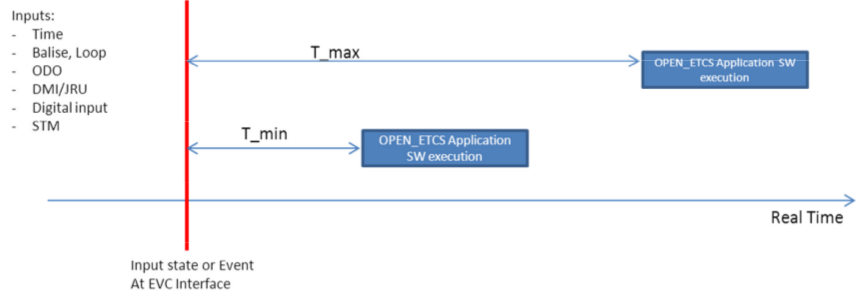
\includegraphics[angle=-0,width=.7\textwidth]{api_2a.png}\\
		\hline\\
		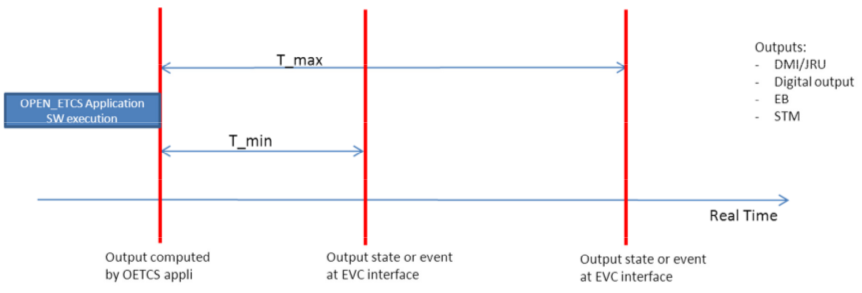
\includegraphics[angle=-0,width=.7\textwidth]{api_1a.png}
	\end{tabular}
	\caption{\emph{Managing delays with time stamps}}
	\label {fig:timestamp}
\end{figure}

Notice that when the input data are time-stamped at the moment they are produced (by the source), the receiving applications may apply a correction in order to manage the delay of transmission of the data; assuming that the clocks of the various calculators are synchronized (e.g. the accuracy of the clock synchronization within
the Model \gls{EVC} is {1ms}).

\chapter{OB subsystem context}
\begin{figure}[H]
	\center
	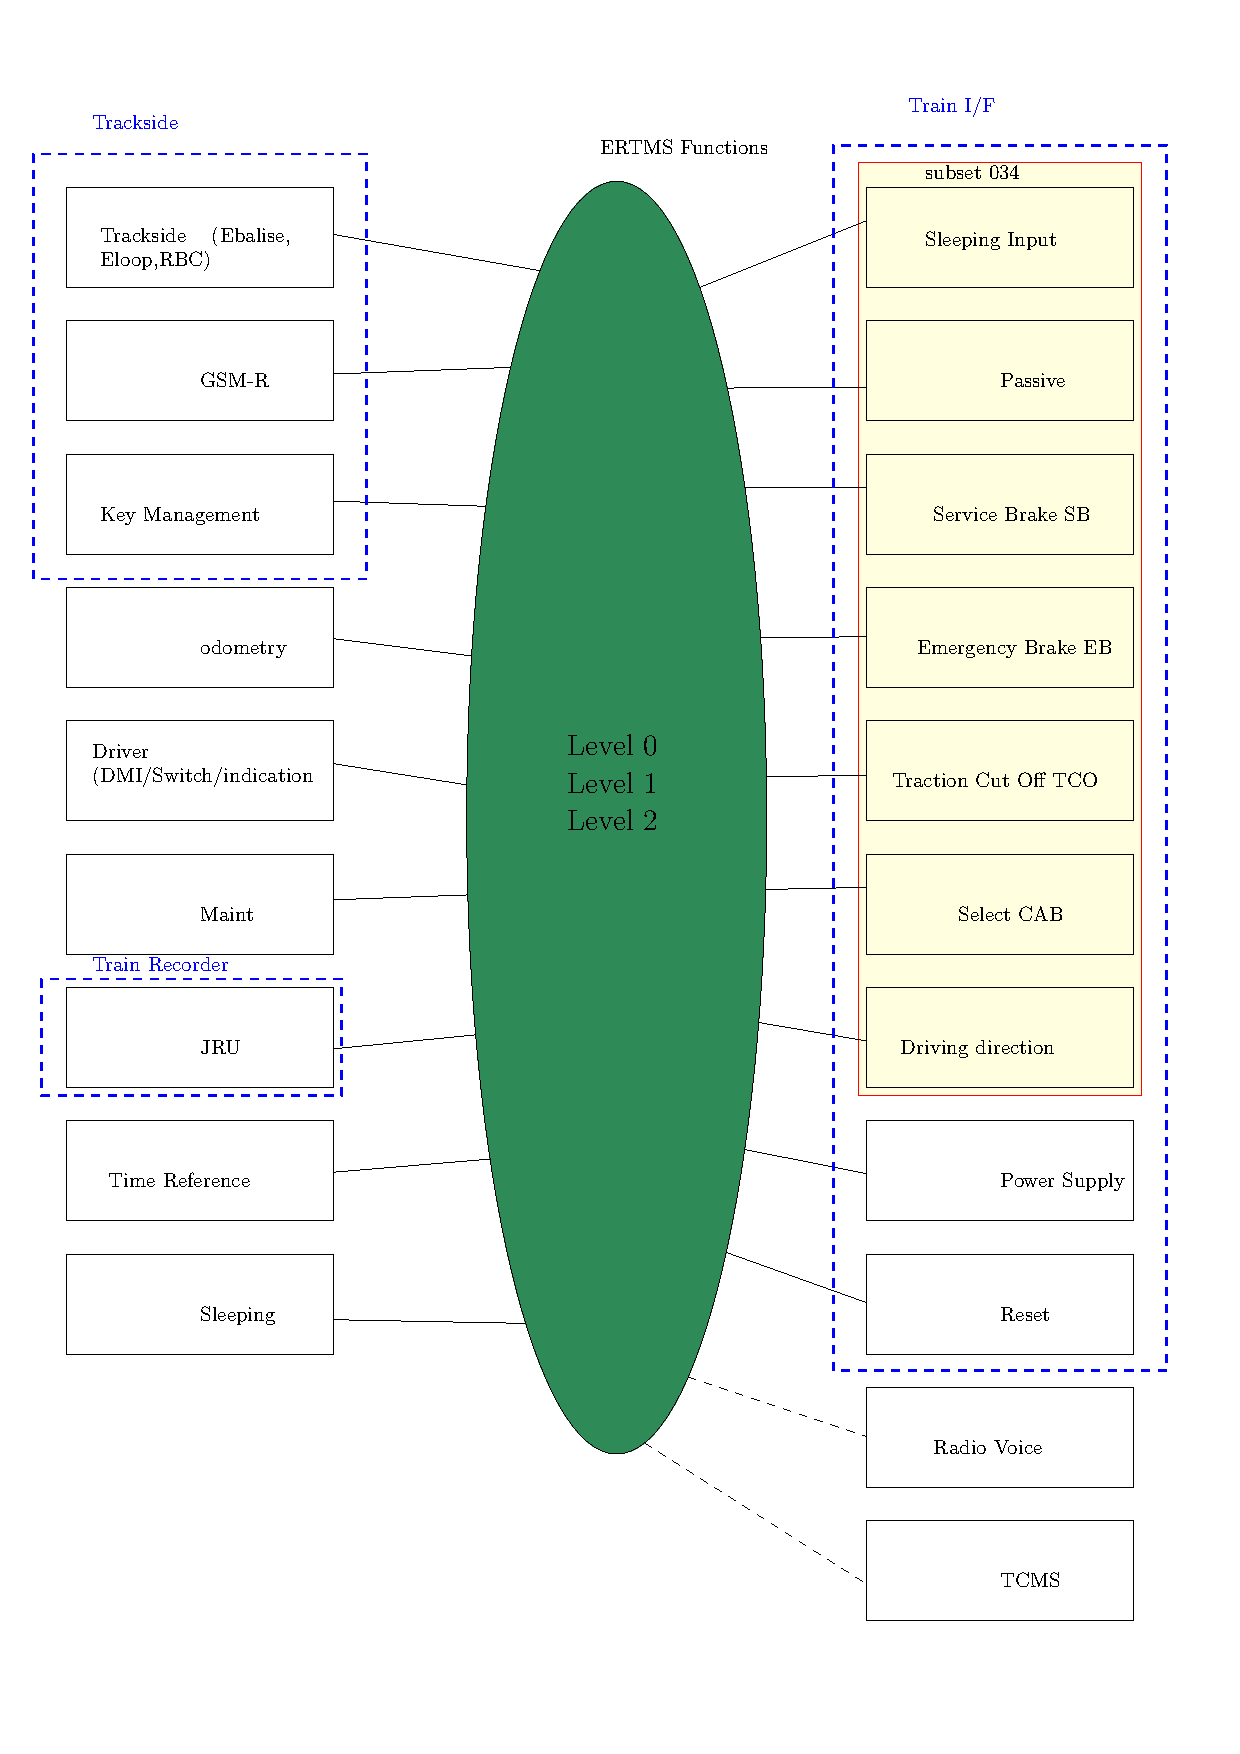
\includegraphics[width=0.7\textwidth]{API_sketch_v1.pdf}
	\caption{OB context diagram}\label{API_sketch}
\end{figure}


\chapter{Elements of the ETCS OB Architecture}

The ERTMS/ETCS OB sub-system comprises at least following equipment’s:

\begin{figure}[H]
	\center
	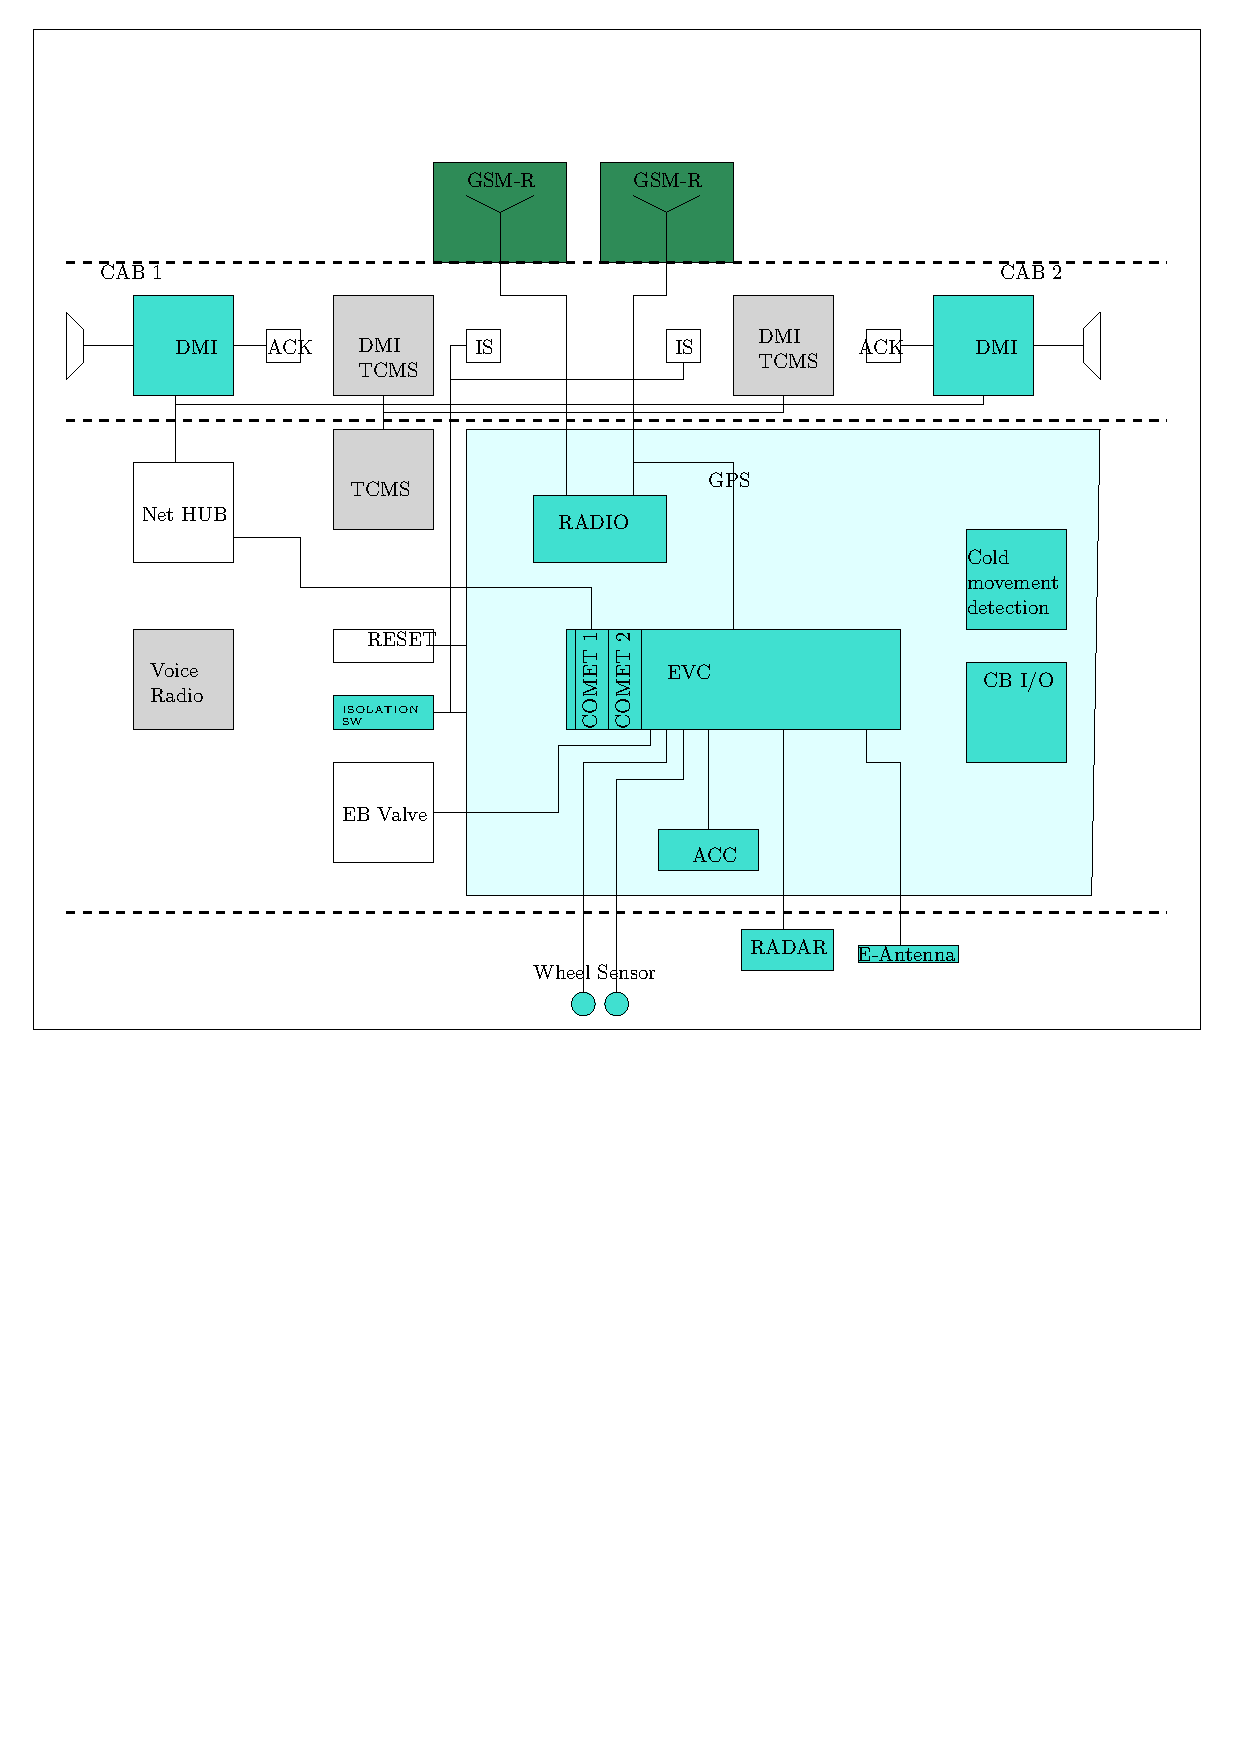
\includegraphics[width=\textwidth]{Arc_over_v1.pdf}
	\caption{OB architecture Overview}\label{Arc_over}
\end{figure}

The ETCS cubicle is realized as one mechanical assembly with a standard housing IP20 and will include :
\begin{itemize} 
	\item the \gls{EVC} (SIL4 equipment);
	\item an internal recorder memory for Juridical Data and diagnostic data;
	\item one GSM-R Data Radio module for GSM-R communication with trackside
	\item relaying devices (contactors, circuit-breakers, relays);
	\item fan modules for the cooling function ;
	\item one accelerometer for the speed and distance measurement; 
	\item a Cold Movement Detector to detect train movements when ETCS is powered off.
\end{itemize}
The \gls{EVC} includes among others the \gls{MMU} providing the odometry function. The odometry implies a complex vital function non mapped on specific Unisig requirements.

Other components installed elsewhere are listed below:
\begin{itemize}
\item  The Isolation switch aims to isolate the ETCS OB sub-system from the train braking and traction interfaces when
ETCS OB is excluded; associated bypass and isolation circuitry is installed to perform the isolation function.
An Isolation indication must be visible to the driver in case of ETCS OB isolation.

\item Reset button
A periodical reset of the ETCS OB sub-system is necessary in order to ensure its required level of availability and safety.

\item One ETCS \gls{DMI}  (including display, loudspeaker and associated acknowledgement button) is installed in each cab. Other components (\gls{EVC}, odometry, radio, ...) can be unique for both cabs or can be installed separately for each cab"


\item The Eurobalise/Euroloop antenna is installed for Eurobalise and Euroloop reception.

\item A radar device is installed for the speed and distance measurement.

\item Wheel Sensors are installed for the speed and distance measurement.

\item Redundant antennas are installed for GSM-R data communication and GPS signal acquisition.
\end{itemize}

A redundant network (bus, switch) is used for the communication between \gls{EVC}, \gls{DMI}(s), \gls{TRU}, and the other OB subsystems.

Train Recorder Unit
The Train Recorder Unit shall record information from the ETCS OB (diagnostic and juridical data) and from the train interfaces. The GPS signal (from a GSM-R/GPS combined antenna) will be received for the data time stamping. 
The TRU will also compute and record the train speed. 
The \Gls{TCMS}  will exchange inputs/outputs information with the \Gls{OB} ETCS OB subsystem

The \gls{TCMS} will manage the \gls{TCMS} \gls{DMI}s and the data communication at train level (between the different vehicles in a multiple configuration). As a remark the \gls{TCMS} and voice radio systems are not part of the ERTMS/ETCS system.

Braking electro-valves, train devices The braking and traction devices commanded by the ETC OB (emergency brakes, service brake and traction cut-off) are part of the Rolling Stock sub-system.

%technical compendium on Odo
\appendix
\chapter{Technical compendium on selected topics}
\section{Concepts and principles of calculation used to estimate train position}

\subsection{conventions and variables related to oriented quantities}

The basic convention for the \gls{MMU}, related to movement detection is given by the rule establishing that the odometric counter values will increase, when the train is moving towards cab A. The Cab A is defined permanently by hard wiring during installation of the \gls{OBU} system. The counter will decrease for the opposite  motion, which is also said to be in direction of Cab B. 
This rule, non depending on any operational setup, makes the counter increase if Cab A is preceding in the movement Cab B when crossing a given track point and vice versa makes the counter decrease when Cab B is preceding cab A.

Counter values of \gls{MMU} are signed, fixed point (1 digit) numbers going from $-15 \cdot 10^6$ to $15 \cdot 10^6$ to be understood as a measure of traveled meters in a given direction, as seen from \gls{OBU}'s (wheel turns) point of view. It should be kept in mind that the value variation of the counter after a given traveled path will fluctuate depending mainly on slip and slide effects. Repeating the train ride on the same track path (length) many times will produce different counter variations at each trial. In general it can be said that the expected fluctuation of the relative counter value will increase with the length of the traveled path.
\begin{figure}[ht!]
\centerline{
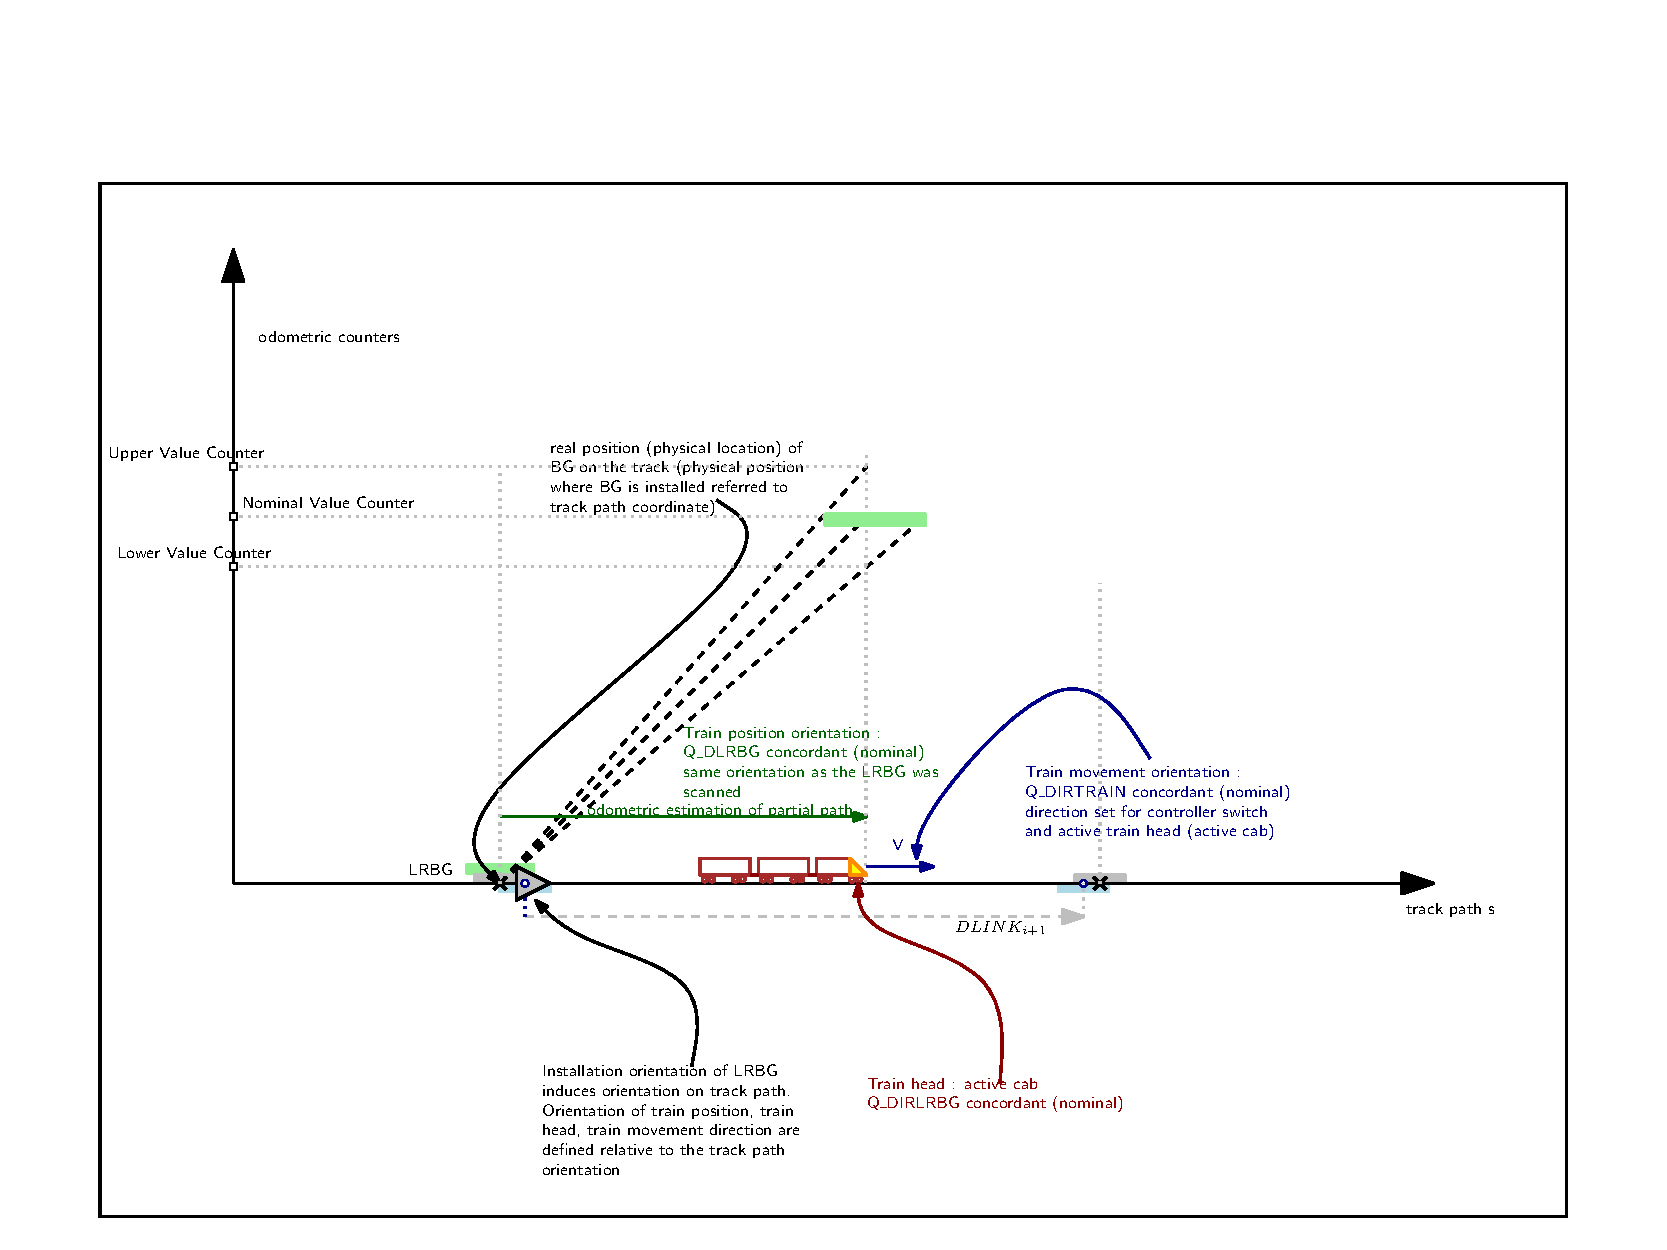
\includegraphics[angle=0,width=0.9\textwidth]{orientation_ontrack_v1.pdf}
}
\caption{\emph{orientation convention}}
\label {fig:orientation}
\end{figure}

The \gls{MMU} is making also movement detection and movement direction detection as reflected by API outputs MOTION\_STATE and MOTION\_DIRECTION. No train movement detection (train standing still) implies also that there will be no train movement direction detection, in such a case the detected train direction is said to be unknown. This outputs will be delayed by the window function needed to stabilize reliable detection. 
The \gls{MMU} orientation establishing the counter behavior is non volatile and non switchable. If in the engine there are two \gls{OBU}s installed then each \gls{OBU} will have it's own wired Cab A irrespective of the configuration adopted for the other \gls{OBU}. The two \gls{OBU}s will never compete for \gls{MMU} data.

When the \gls{OBU} is in a mode referencing to a LRBG, the directions relevant for train driving are given by the following triple (relative to LRBG orientation):
\begin{itemize}
\item Q\_DIRLRBG Train Orientation => active cabin, => Front End => headlights
\item Q\_DIRTRAIN direction of train movement (not the detected motion direction but the direction as set by direction controller switch.
When reversing is allowed this orientation can be reverted operating on the direction switch allowing the train to proceed in reverse direction)  possible values are : nominal (e.g. train oriented nominal and direction switch forward), reverse (e.g. train orientation nominal and direction switch reverse) unknown direction switch in neutral position. The ETCS system will supervise the direction of motion and allow to switch in the reverse direction (opposite to train direction) only under foreseen conditions e.g. during emergency in tunnel.
\item Q\_DLRBG "scanning" orientation at time of over-passing the LRBG and therefore "sign" of the coordinate relative to LRBG (positive coordinate direction means train has scanned LRBG in nominal direction reading increasing N\_PIGs and is now on the arrow tip side of LRBG). The absolute value of this coordinate is given by the variable D\_LRBG.
\end{itemize}
The above three quantities have to be considered as software variables, that need to be initialized and may change depending on the actual state and inputs elaborated. They have only meaning if the direction of the LRBG is given.

other relevant Direction qualifier are :
\begin{itemize}
\item Q\_DIR message orientation (relative to sending BG) nominal (message valid for nominal scanning/overpassing of the BG) reverse and neutral (valid for both directions) In case of RBC sending the message the reference orientation is given by the one of the LRBG.
This direction qualifier is most relevant for giving the relative position of a MA (Packet 12) transmitted by a BG  in respect to relevant train end. This gives the permitted movement direction of the train, and if an opposite movement direction is detected, by evaluating the \gls{MMU} output MOTION\_DIRECTION a brake command should be triggered.
\item Q\_LINKORIENTATION part of a linking vector (packet 5) indicates if the linked BG pointed by the vector will be over-passed in nominal or reverse direction.
\end{itemize}


other Direction qualifier are :
\begin{itemize}
\item Q\_MPOSITION orientation of kilometer counting convention
\item Q\_ORIENTATION orientation given by RBC to a passed LRBG
\end{itemize}

\clearpage

\subsection{Rail-routed path and empirical odometric map}
The estimation of the train position is currently based on the odometric measure of the distance traveled by the train made with an on board equipment and by the detection of reference balises installed at known positions on the track, when the Balise receiver antenna detects them. 
The distance is measured along the rail or track path. Actually track routes can have variable branches (when crossing switch points from blade side). The on-board odometry is not able to map different branches and will only trace an one-dimensional path.

\begin{figure}[!ht]
%\boxed{
\centerline{
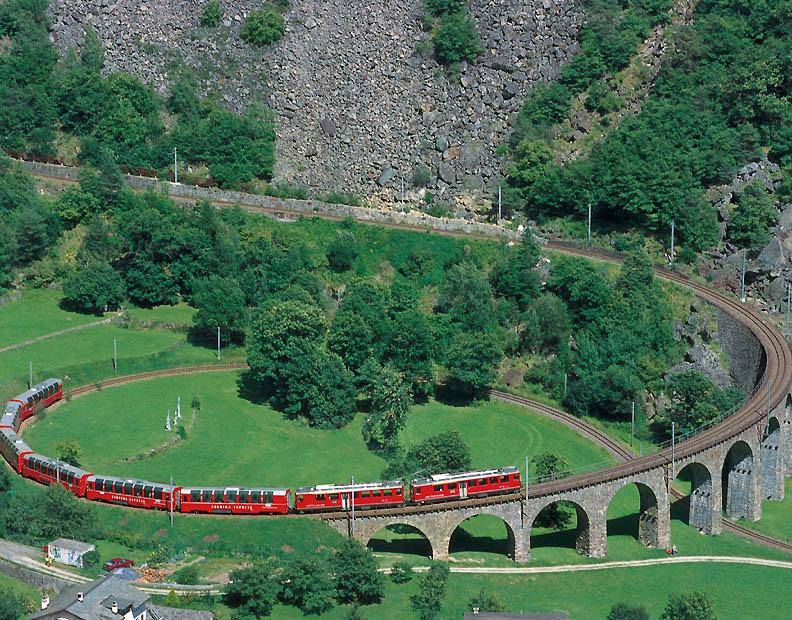
\includegraphics[angle=-0,width=.38\textwidth]{Brusio_RSLB.jpg}
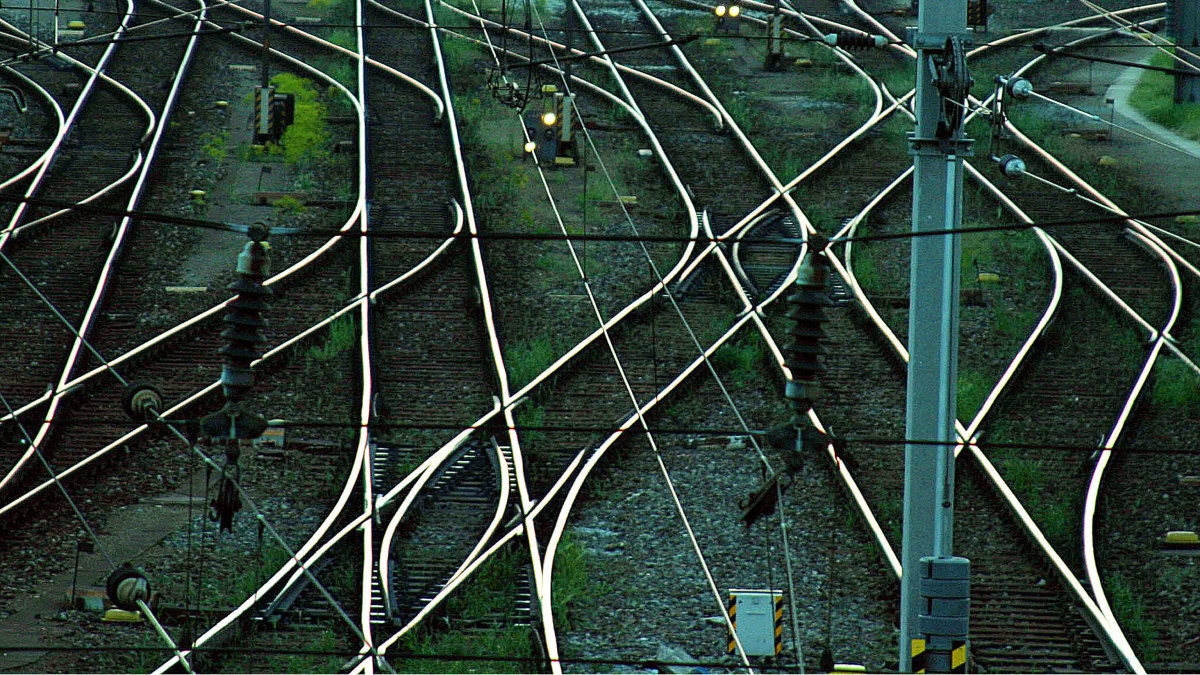
\includegraphics[angle=-0,width=.53\textwidth]{deviate.jpg}
}
%}
\caption{\emph{Examples of train path}}
\label {fig:trainpath}
\end{figure}
The picture in figure \ref{fig:trainpath} gives two illustrative examples of rail path.
Even if the train route can follow different branches depending on the position of the switches the coordinate system available on-board is always one-dimensional and needs to get updated track data for the selected route each time the train passes over a switch point from blade side. 

This is done mainly through the so-called repositioning information\footnote{see \gls{SRS} 026 3.8.5.3.5.} available at a BG immediately after the branch point. Such a balise group is usually announced by a weak link \footnote{3.4.4.2. and 3.4.4.4.} not including the id\footnote{id number 16383 } of the BG and applying a relaxed expectation window.
\begin{figure}[!ht]
\centerline{
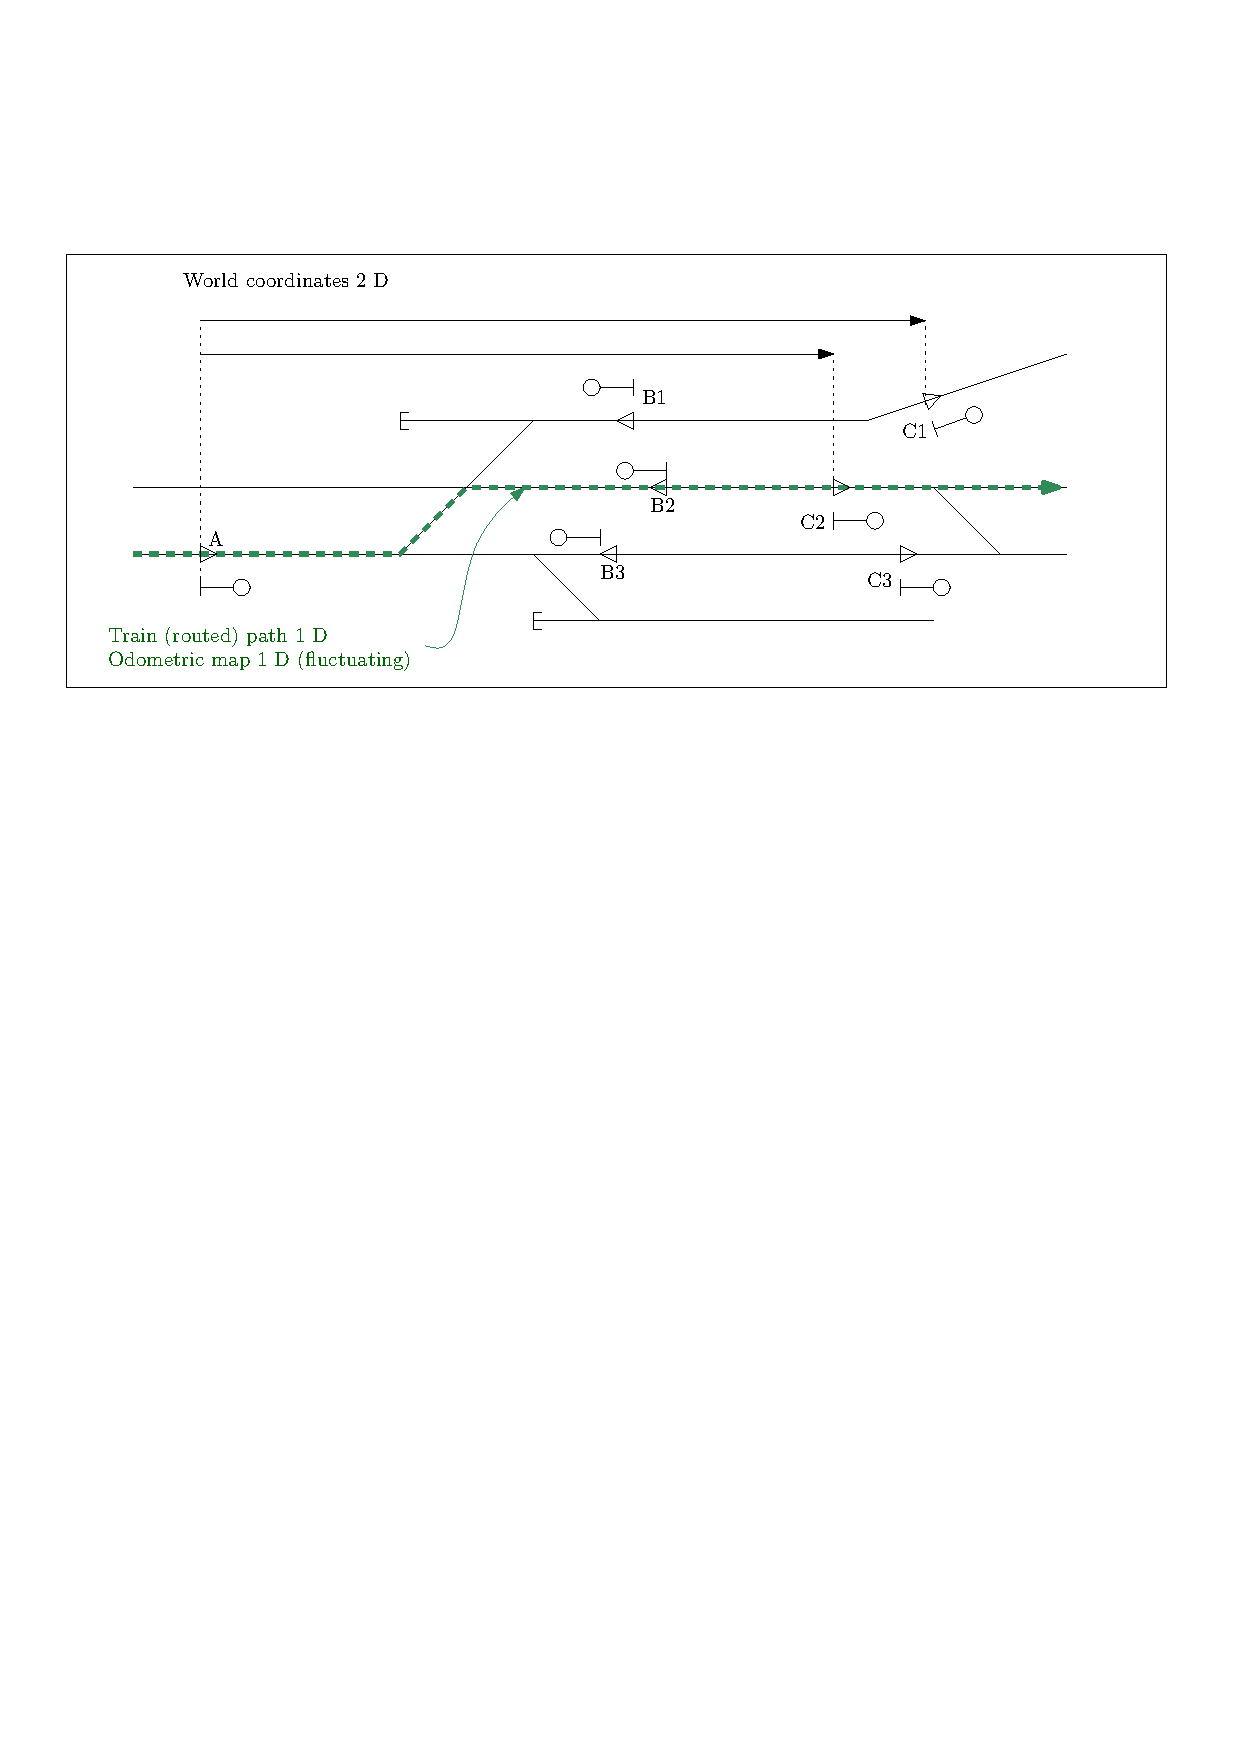
\includegraphics[angle=-0,width=.8\textwidth]{trainroute_v2.pdf}
%\includegraphics[angle=-0,width=.5\textwidth]{fig24_v1.png}
}
\caption{\emph{Example of repositioning data.}}
\label {fig:Fig24}
\end{figure}
Note: In cases where a balise group contains repositioning \footnote{By convention \emph{relocation} indicates a coordinate shift along the the train path, while \emph{repositioning} indicates a displacement in the second dimension, which is not tracked by the on-board equipment} information, the term linked also applies since the balise group is announced, marked as linked and contains repositioning information marked accordingly. For clarity sometimes we will use the term weakly linked. Repositioning information contained in a balise group message shall only be evaluated if linking information has announced a following balise group as unknown but containing repositioning information. A balise group message containing a movement authority shall not contain repositioning information for the same direction.

In the balise group A the following information is given:
\begin{itemize}
\item The most restrictive track description from all routes (which could be a combination
from the routes);
\item The linking distance given to the farthest balise group containing repositioning
information, the identification of the repositioning balise group is not known;
\item For a given aspect of signal A, the most restrictive MA from all routes (the shortest
sections from the routes and the lowest target speed at the End Of Authority);
\item If some sections are time limited, the most restrictive timer.
\end{itemize}
Balise groups B (B 1 or B 2 ) give the following static information (repositioning information):
\begin{itemize}
\item Linking to the next balise group C
\item The distance to the end of the current section (i.e. the distance to the end of section
B1 - C1, or the distance to the end of section B2 - C2)
\item The track description related to this track.

\end{itemize}

\subsubsection{Mitigation of balise cross-talk while expecting repositioning information}
If repositioning is announced and the expected repositioning balise group has been found, the ERTMS/ETCS on-board equipment shall keep looking for a balise group that satisfies the same criteria as this previously expected and already found
repositioning balise group, until one of the following events occurs:
\begin{itemize}
\item the on-board antenna leaves the expectation window of the repositioning balise group that was announced and already found
\item a linked balise group that has been announced with known identity is found.
\end{itemize}
If a second balise group is found that satisfies the same criteria as the previously
expected and already found repositioning balise group, the ERTMS/ETCS on-board
equipment shall command the service brake and the driver shall be informed. At
standstill, the location based information stored on-board shall be shortened to the
current position. Refer to appendix Subset 026 A.3.4 for the exhaustive list of information, which shall be shortened.

Note: this function is independent from linking function, i.e. the rules related to
linking always apply. This means that once a repositioning balise group has been found and if this latter contains new linking information, the ERTMS/ETCS on-board equipment will start expecting the first balise group announced in this new linking information in parallel with the monitoring specified for mitigating balise reception degradation


\subsection{Correlating two linked BG detections}
%\begin{figure}[!ht]
%\centerline{
%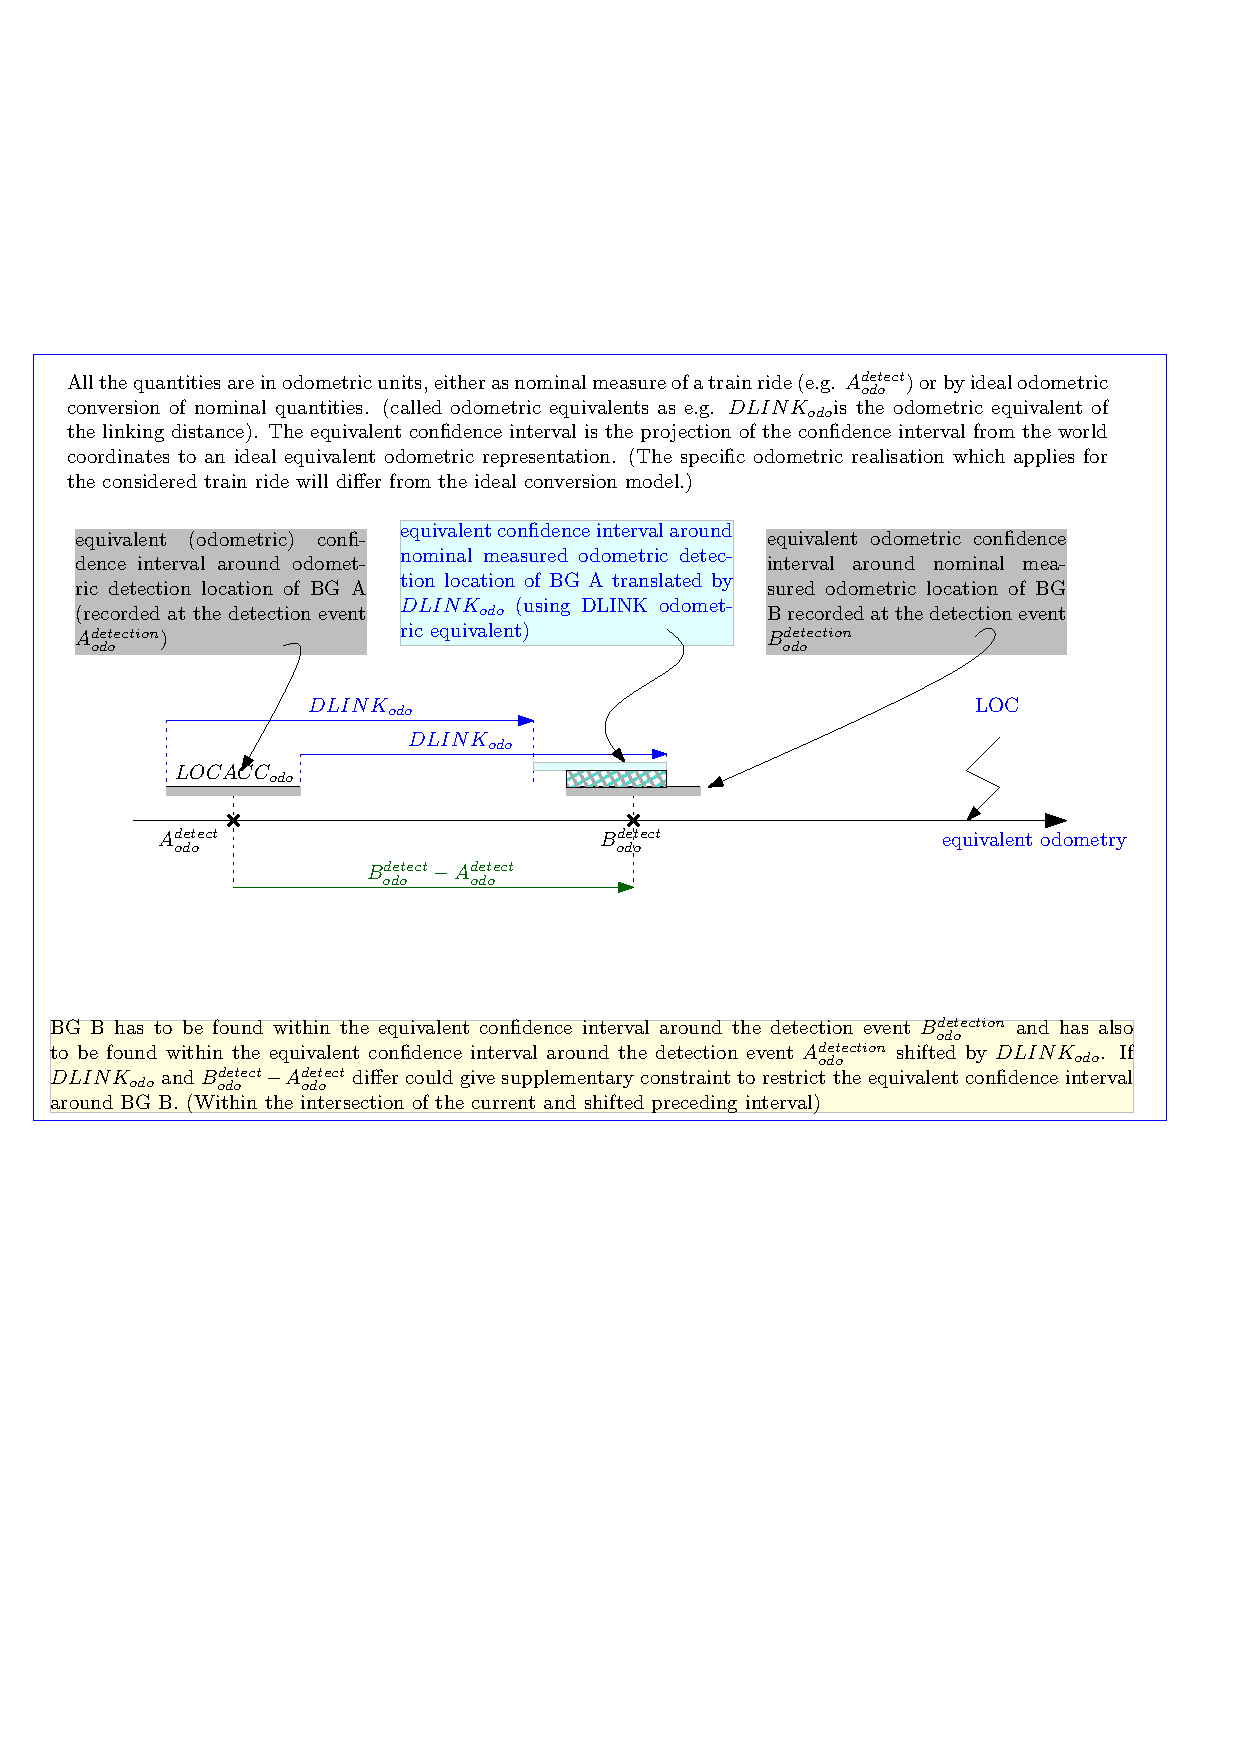
\includegraphics[angle=0,width=.9\textwidth]{odomap_v1.pdf}
%}
%\caption{\emph{Supplementary information}}
%\label {fig:odomap}
%\end{figure}
If the odometric difference between two linked BG detections differs from nominal distance in a significant way (at least more than the odometric error of 5 \% in plus or in minus) this supplemental information can be used to constrain the reciprocal confidence interval of the second detected BG.


\subsection{Odometry from Wheel motion}

In the following we try to adopt an uniform symbol convention, based on the assumption that there are quantities measured at fixed time intervals and quantities measured at variable, speed dependent time intervals. Fixed time intervals are :
\begin{equation}
\tau^\star =1\, \mu s ,\,
\tau^\circ = 50 \,ms, \,
\tau^\bullet = N^\bullet \tau^\circ = 500\, ms
\end{equation}
Variable time intervals are given by the time between the detection of two odometer teeth or two odometer virtual teeth.

\begin{figure}[!ht]
\centerline{
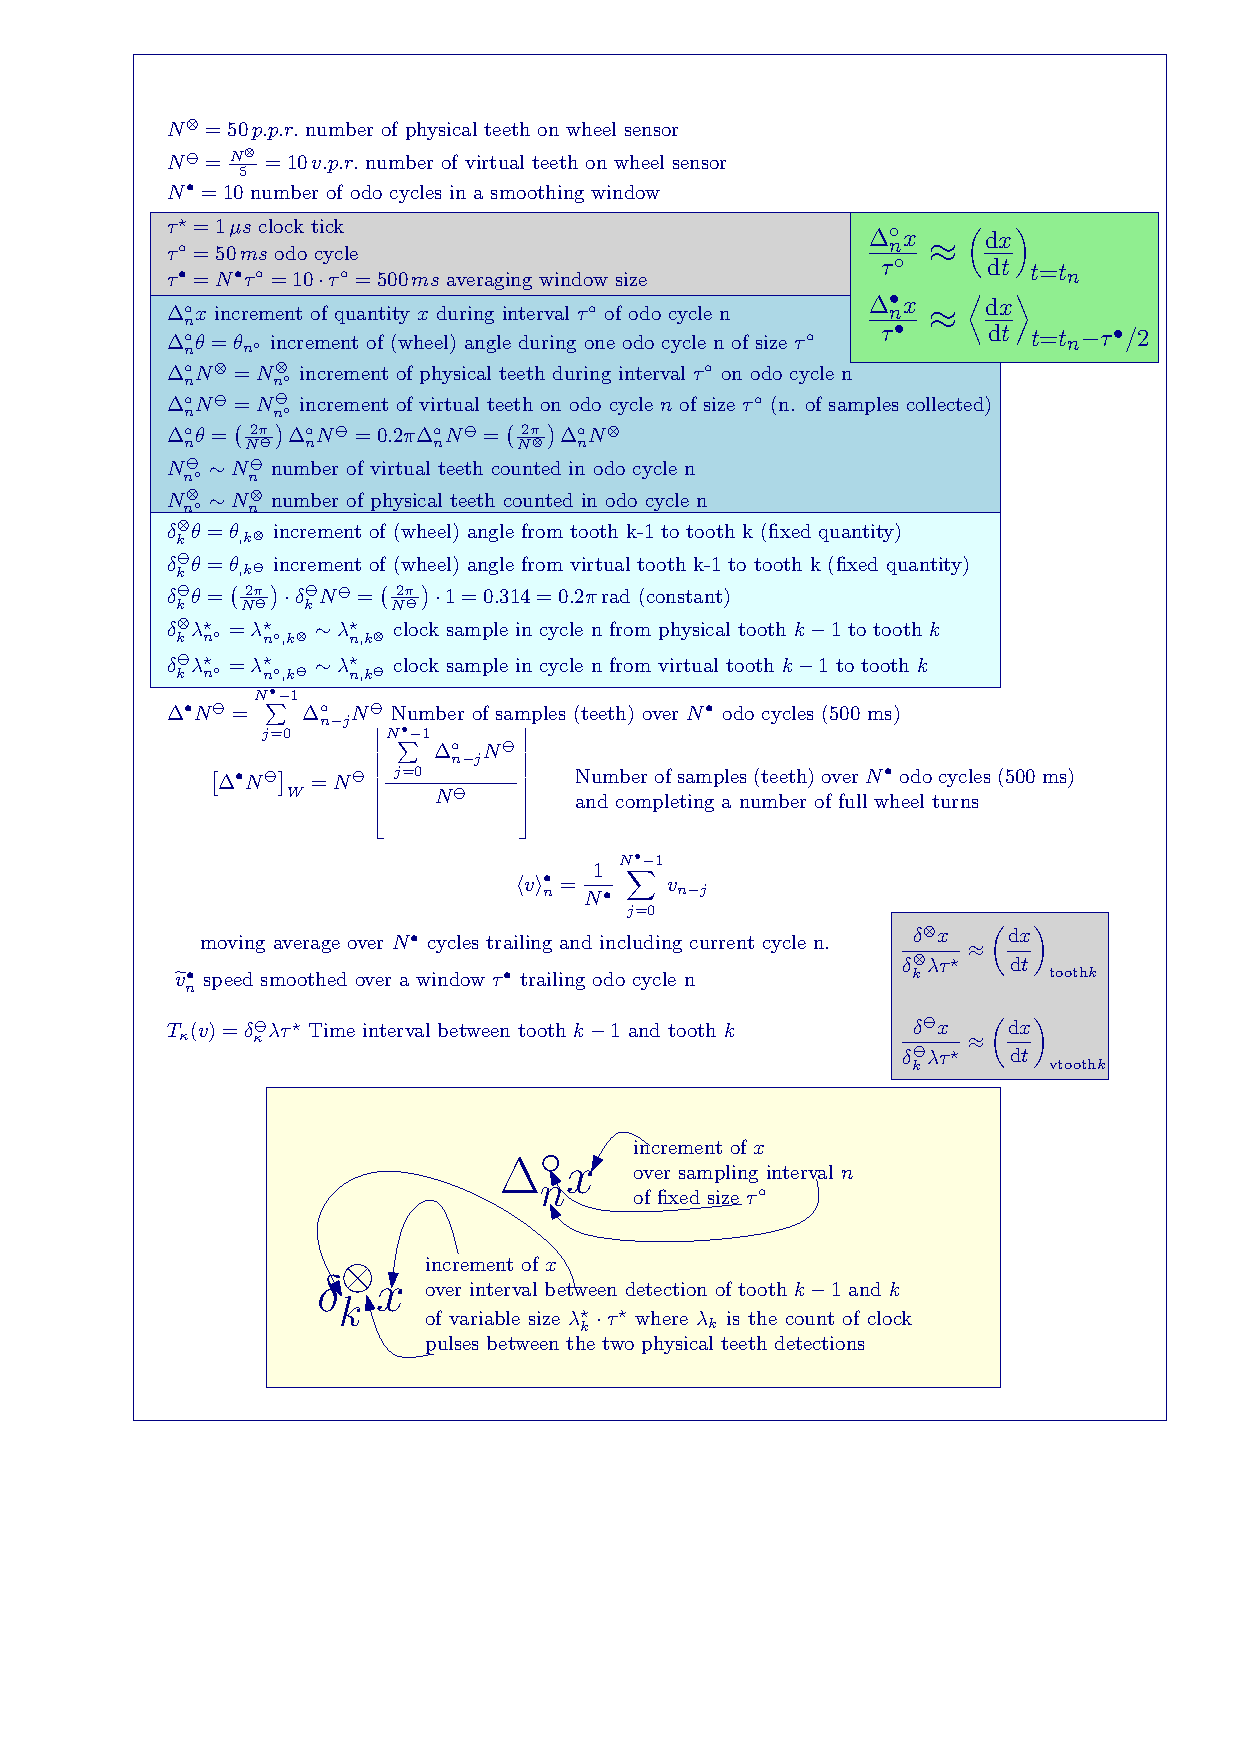
\includegraphics[angle=0,width=.95\textwidth]{symbols_used_v2.pdf}
}
\caption{\emph{explanation to symbols used in following text}}
\label {fig:symbolu}
\end{figure}
\begin{figure}[!ht]
\centerline{
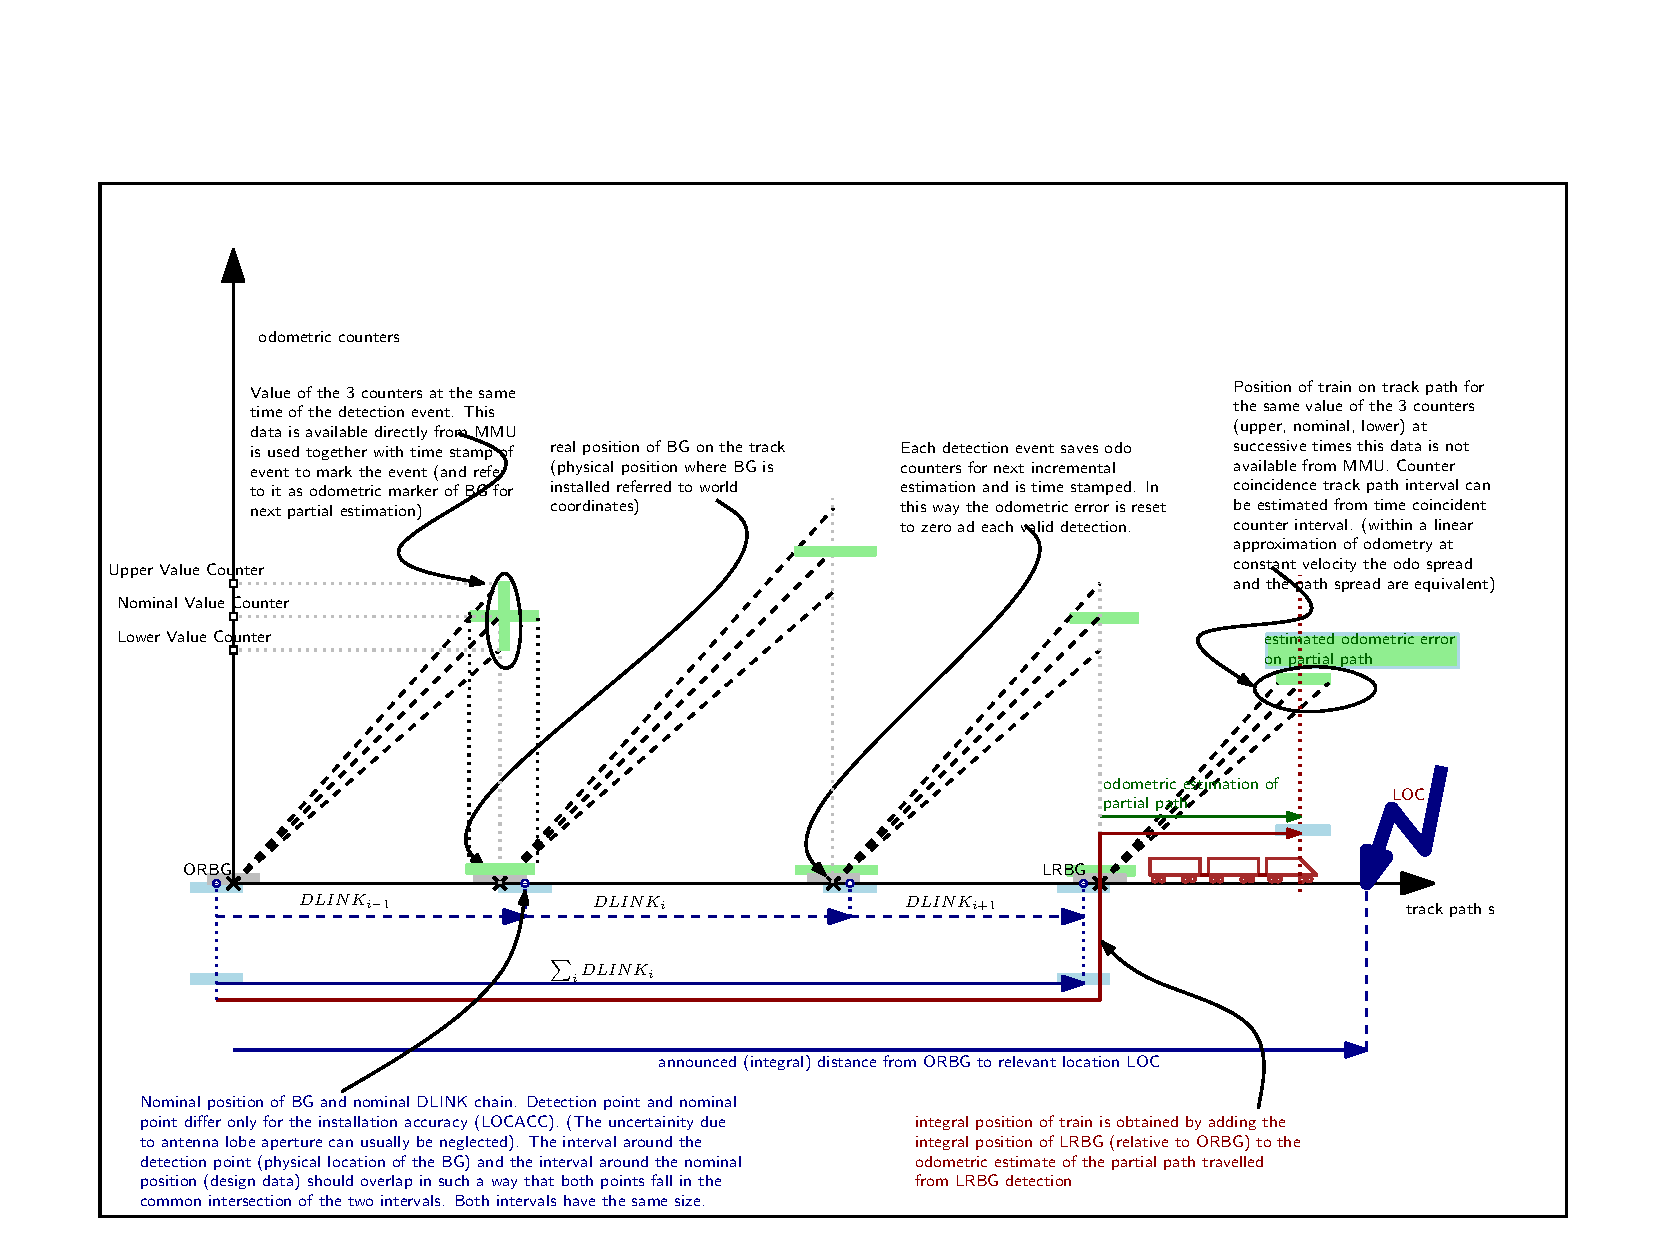
\includegraphics[angle=0,width=1.\textwidth]{odo_linear_II.pdf}
}
\caption{\emph{odometric conversion}}
\label {fig:odoconv}
\end{figure}
\subsubsection{Basic principles for odometry modeling}
The main role/function of the \gls{MMU}  involves acquiring the measured physical quantities on the various sensors, to process
them and to supply, in safety, to each EVC main unit the following set of information:
\begin{itemize}
\item A speed range [speed min , speed nom , speed max ].
\item A cumulated distance range [distance min , distance nom , distance max ].
\item An acceleration range [acceleration min , acceleration nom , acceleration max ].
\item The direction of travel (\gls{DOT}).
\item The motion information.
\item The adhesion loss detection.
\end{itemize}
\newpage
\subsubsection{Odometry model performance}

\begin{tabular}{|l| l|}
\hline
Measure / Estimate  & examples of range / value for an odometry model\\
\hline
Distance accuracy & $\pm$(4m + 5\%) \\
\hline
Speed accuracy & $\pm$ 2 km/h for v$<$ 30 km/h, \\ 
&then increasing linearly up to $\pm$ 12 km/h at v = 500 km/h \\
\hline
%\colorbox{yellow}
{Speed \emph{resolution}} 
%(DESG 0648\_105) 
& $\frac{2\pi R}{N^\ominus\cdot \tau^\circ } = \frac{0.314 m}{.05 s}\,  (\approx 6.28\, m/s \approx 22.6\, km/h)$ \\ & minimal speed to have at least one new sample each cycle\\
\hline
data acquisition cycle $\tau^\circ$ &  50 ms between measurement \\
\hline
Cycle time  & Data transmission to Core each 100 ms\\
\hline
Distance resolution & 0.34 m (min for standstill detection = 0.5 m)\\
\hline
Speed resolution (GATC DESG 0638) & 0,025 m/s $(\approx 0.1\, \mathrm{km/h} )$ \\
\hline
Speed range & 0 to 500 km/h \\
\hline
Direction of travel (\gls{DOT}) &Mandatory in objective SIL4\\
\hline
 Motion detection & Motion detected if v $>$ 0,5 km/h max or d $>$ 0,5 m max \\
\hline
 Safety Integrity Level & SIL4\\
\hline

\end{tabular}

\subsubsection{Encoders and \gls{WS}}

Incremental encoders provide a specific number of equally spaced pulses per revolution (PPR) or per inch or millimeter of linear motion. A single channel output is used for applications where sensing the direction of movement is not important. 
\begin{figure}[ht!]
\centerline{
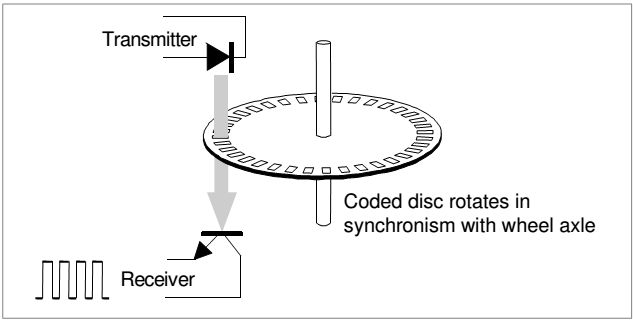
\includegraphics[angle=0,width=.5\textwidth]{impulsweggeber.jpg}
}
\caption{\emph{wheel sensor}}
\label {fig:wsens}
\end{figure}
Where direction sensing is required, quadrature output is used, with two channels 90 electrical degrees out of phase; circuitry determines direction of movement based on the phase relationship between them. This is useful for processes that can reverse, or must maintain net position when standing still or mechanically oscillating. For example, machine vibration while stopped could cause a unidirectional encoder to produce a stream of pulses that would be erroneously counted as motion. The controller would not be fooled when quadrature counting is used.

When more resolution is needed, it is possible for the counter to count the leading and trailing edges of the pulse train from one channel, which doubles (x2) the number of pulses counted for one rotation or inch of motion. Counting both leading and trailing edges of both channels will give 4x resolution.
\begin{figure}[ht!]
\centerline{
%\includegraphics[angle=0,width=.35\textwidth]{counting.png}
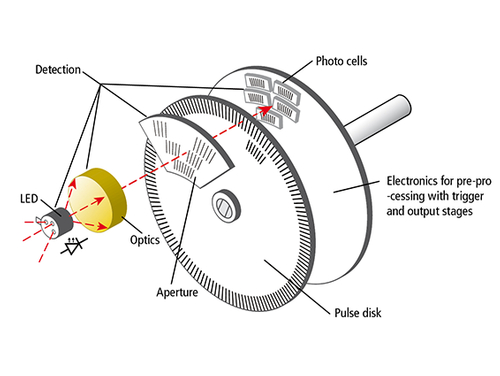
\includegraphics[angle=0,width=.35\textwidth]{increm_det_en.png}
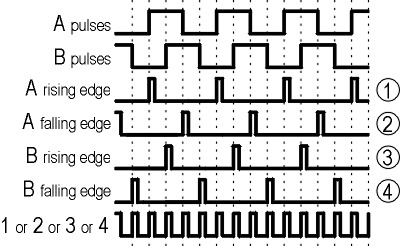
\includegraphics[angle=0,width=.35\textwidth]{quad.jpg}
}
\caption{\emph{encoder output}}
\label {fig:ienc}
\end{figure}
An incremental encoder’s output indicates motion. To determine position, its pulses must be accumulated by a counter. The count is subject to loss during a power
interruption or corruption by electrical transients. When starting up, the equipment must be driven to a reference or home position to initialize the position counters. Some incremental encoders also produce another signal known as the “marker,” “index,” or “Z channel.” This signal, produced once per revolution of a shaft
encoder or at precisely-known points on a linear scale, is often used to locate a specific position, especially during a homing sequence.
Resolution is the number of measuring segments or units in one revolution of an encoder shaft or one inch or mm of a linear scale. Shaft encoders are available with
resolutions up to 10,000 pulses per revolution (PPR) directly, and 40,000 PPR by edge-detection of the A and B channels, while linear encoders are available with
resolutions measured in microns. 
The bottom line is, the selected encoder must have resolution equal to or better than that required by the application. But resolution is not the whole story. Accuracy and resolution are different, and it is possible to have one without the other. This figure shows a distance X divided into 24 increments or “bits.” If X represents $360\deg$ of shaft rotation, then one revolution has been resolved into 24 parts.
\begin{figure}[ht!]
\centering
\begin{tabular}{c}
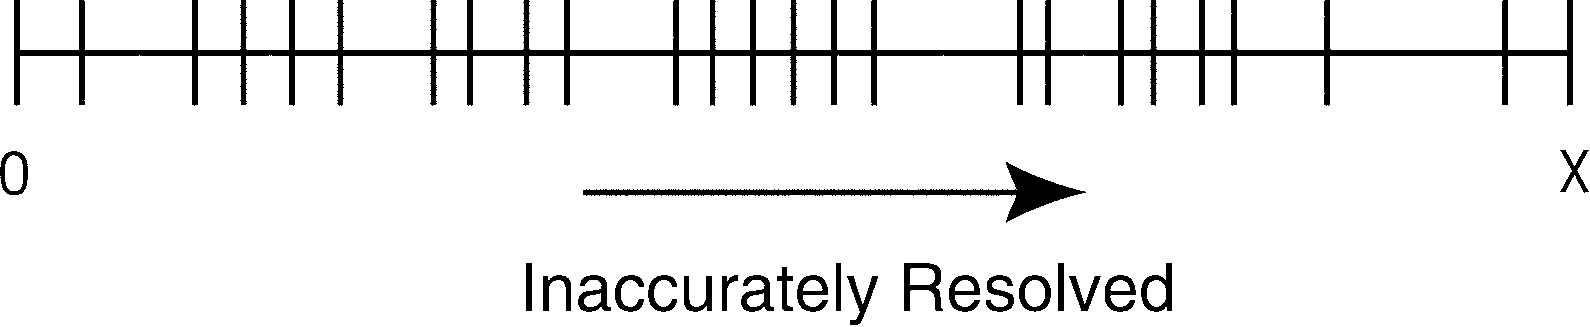
\includegraphics[angle=0,width=.5\textwidth]{accuracy.png} \\
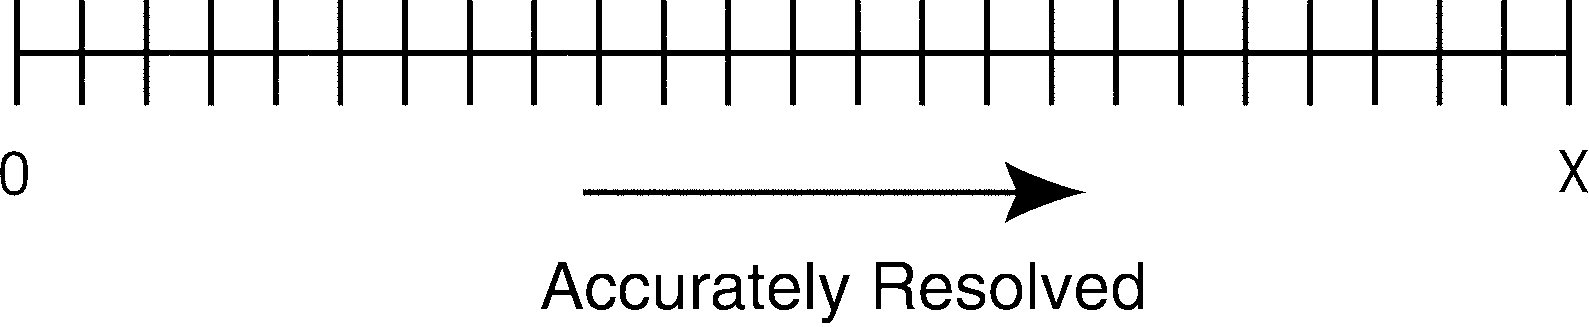
\includegraphics[angle=0,width=.5\textwidth]{accuracy2.png}
\end{tabular}
\caption{\emph{accuracy}}
\label {fig:encaccu}
\end{figure}
While there are 24 bits of resolution, the 24 parts are not uniform. This transducer could not be used to measure position, velocity or acceleration with any accuracy. On the other hand, in this figure the distance X is divided into 24 equal parts. Each increment represents exactly 1/24 of a revolution. This transducer operates with accuracy as well as resolution. Accuracy, however, can be independent of resolution. A transducer may have a resolution of only two parts per revolution, yet its accuracy could be $\pm 6$ arc seconds.

System Accuracy: An encoder performance is typically stated as resolution, rather than accuracy of measurement. The encoder may be able to resolve movement into precise bits very accurately, but the accuracy of each bit is limited by the quality of the machine motion being monitored. For example, if there are deflections of machine elements under load, or if there is a drive screw with 0.1 inch of play, using a 1000 count-per-turn encoder with an output reading to 0.001 inch will not improve the 0.1 inch tolerance on the measurement. The encoder only reports
position; it cannot improve on the basic accuracy of the shaft motion from which the position is sensed.

System Repeatability: Repeatability is the tolerance to which the controlled machine element can be repeatedly positioned to the same point in its travel. Repeatability is generally less than system resolution, but somewhat better than system accuracy. 10,000 pulses per turn can be generated from a 2500 cycle, two channel encoder. Typically with a Dynapar encoder, this 4x signal will be accurate to better than $\pm 1$ count.

Resolution is the ability to 'resolve' differences; that is, to draw a distinction between two things. High resolution means being able to resolve small differences. In a digital system, resolution means the smallest increment or step that can be taken or seen. In an analog system, it means the smallest step or difference that can be reliably observed. 

The accuracy of a system refers to how much the system, whether in measurement or control, deviates from the truth. To be meaningful, accuracy must really refer to 'worst case accuracy'.
As a trivial example, a stopped, unworking clock is still correct twice a day! We must describe this unworking clock by its worst case accuracy, which would be +/- 6 hours. Sometimes the '+/-' is dropped and the extent of the inaccuracy is reported: for this clock, it would be 12 hours.
Beyond describing the worst case, we must also consider resolution. The following is very important:
The accuracy of a system can never exceed its resolution! This follows from the worst case requirement.

Repeatability is the variance in repeated measurements on an unchanging sample. If measured statistically, it is sometimes referred to as the noise level in the measurement. In general, high repeatability means a low noise level. Precision is used in different ways depending on context.
By design, measurement resolution is normally set better than accuracy. In the case of contact angle measurements, the resolution might be 0.01 degree but the absolute accuracy 1 degree. Why have resolution better than accuracy? One reason is that often accuracy is limited by the availability of calibration standards to show or prove the accuracy. If the best available standard is +/- 0.5 degrees, you can not claim an accuracy better than that. However, the ability to measure small differences between samples, whatever the absolute number, is useful and for this reason a higher resolution is provided. In general, instruments can measure repeatedly the same sample with a variance of a few units of resolution. This is called the noise level of the measurement. If we report a resolution of 0.01 degree, we expect to measure a static sample with a repeatability of, say, +/-0.02 or 0.03 degrees. 

\subsection{Speed measure}
The\footnote{Petrella Speed Measurement Algorithms for Low-Resolution Incremental Encoder Equipped Drives: a Comparative Analysis \cite{petrella}} classical and probably the simplest method to measure rotor speed is the direct measure of the frequency of the encoder pulses. 

\begin{figure}[ht!]
\centerline{
%\includegraphics[angle=0,width=.35\textwidth]{counting.png}
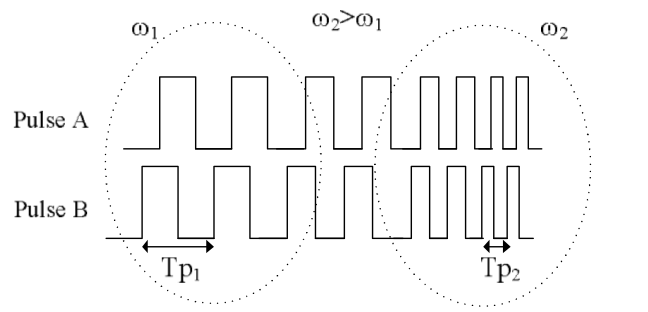
\includegraphics[angle=0,width=.5\textwidth]{speed_var.png}
}
\caption{\emph{encoder output while speed increases}}
\label {fig:v-var}
\end{figure}
Typically the number of the observed pulses inside a given and constant-width time-window is counted. Angular speed is then approximated to the discrete incremental ratio, that is constant speed is considered inside the observation windows:
\begin{equation}
\omega=\frac{\mathrm{d}\theta}{\mathrm{d}t}\approx\frac{\Delta_{n}^\circ\theta}{\tau^\circ}=\left(\frac{2\pi}{N^\otimes }\right) \frac{\Delta_n^\circ N^\otimes}{\tau^\circ}
\end{equation}

Where $N^\otimes$ is the number of pulses per revolution, $\Delta^\circ_n \theta$ is the angular increment and $\Delta^\circ_n N$ the corresponding number of pulses counted within the cycle n corresponding (observation window of fixed size $\tau^\circ$).  As a concrete model we assume to have following values $ N^\otimes = 50 \,\mathrm{p.p.r.} $ (pulses per revolution) a wheel diameter of about $ R \approx 1\, \mathrm{m}$ (ICE trains have about 980 mm, while Euro-sprinter are between 1.1 and 1.2m) at $\varv_{train} = 5 \mathrm{km/h}=1.4 \,\mathrm{m/s}$
whith $\tau^\circ=50 \, m\mathrm{s}$ we get:
\begin{equation}
\boxed{
\Delta_n^\circ N^{\otimes}= \varv_{train}[m/s]\cdot \left(\frac{\tau^\circ}{2\pi R}\right)\cdot N^\otimes=1.4\cdot\frac{0.05}{3.14}\cdot 50 = 1.4\cdot \left(0.796\right) =1.1 }
\end{equation}

We observe that at low speeds there will be no increment in pulse counter $\Delta^\circ_n N^\otimes$ within the observation window $\tau^\circ$ (no variation is detected in one single \gls{MMU} cycle, the counter may vary after more than one \gls{MMU} cycle).
%$\mathfrak{N} \!\!\!\!\backslash $  $ \check{N} N^{\bullet}$

\begin{tabular}{|l|l | l| l|}
\hline
speed $\varv$ [km/h] &speed $\varv$ [m/s]&  approximate pulse (teeth) count & virtual teeth \\ &  & in a $50\,\mathrm{m}s $ time window ($\varv \cdot 0.796$) & $\Delta_n^\circ N/5$\\
\hline
$\varv_{train}\approx 1\, \mathrm{km/h}$ & 0.28 m/s & $\Delta_n^\circ N^\otimes\approx 0.22 $ & $\Delta_n^\circ N^\ominus \approx  .044 $ \\
\hline
$\varv_{train}\approx 3.6\, \mathrm{km/h}$ & 1 m/s & $\Delta_n^\circ N^\otimes\approx 0.796 $ & $\Delta_n^\circ N^\ominus \approx  .159 $\\
\hline
$\varv_{train}\approx 5\, \mathrm{km/h}$ & 1.4 m/s & $\Delta_n^\circ N^\otimes\approx 1.1 $ & $\Delta_n^\circ N^\ominus \approx  .22 $ \\
\hline
$\varv_{train}\approx 10\, \mathrm{km/h}$ & 2.8 m/s & $\Delta_n^\circ N^\otimes\approx 2.2 $ & $\Delta_n^\circ N^\ominus \approx  .44 $ \\
\hline
$\varv_{train}\approx 11.3\, \mathrm{km/h}$ & 3.14 m/s & $\Delta_n^\circ N^\otimes\approx 2.5 $ & $\Delta_n^\circ N^\ominus \approx  .5$ \\
\hline
%\colorbox{yellow}
{$\varv_{train}\approx 22.6 \,\mathrm{km/h}$} & 6,28 m/s &
%\colorbox{yellow}
{ $\Delta_n^\circ N^\otimes\approx 5 $} & $\Delta_n^\circ N^\ominus \approx  1 $\\
\hline
$\varv_{train}\approx 36\, \mathrm{km/h}$ & 10 m/s & $\Delta_n^\circ N^\otimes\approx 7.96 $ & $\Delta_n^\circ N^\ominus \approx  1.59 $\\
\hline
$\varv_{train}\approx 50\, \mathrm{km/h}$ & 14 m/s & $\Delta_n^\circ N^\otimes\approx 11 $ & $\Delta_n^\circ N^\ominus \approx  2.2$ \\
\hline
$\varv_{train}\approx 72 \,\mathrm{km/h}$ & 20 m/s & $\Delta_n^\circ N^\otimes\approx 15.92 $ & $\Delta_n^\circ N^\ominus \approx  3.18$\\
\hline
$\varv_{train}\approx 100 \,\mathrm{km/h}$ & 28 m/s & $\Delta_n^\circ N^\otimes\approx 22 $ & $\Delta_n^\circ N^\ominus \approx  4.4 $\\
\hline  
$\varv_{train} \approx 150\, \mathrm{km/h}$ & 42 m/s & $\Delta_n^\circ N^\otimes\approx 33 $ & $\Delta_n^\circ N^\ominus \approx  6.6 $\\
\hline
$\varv_{train}\approx 160 \,\mathrm{km/h}$ & 44.8 m/s & $\Delta_n^\circ N^\otimes\approx 35.66 $ & $\Delta_n^\circ N^\ominus \approx  7.132$ \\
\hline
$\varv_{train}\approx 300\, \mathrm{km/h}$ & 84 m/s & $\Delta_n^\circ N^\otimes\approx 66.864 $ & $\Delta_n^\circ N^\ominus \approx  13.372 $\\
\hline
$\varv_{train}\approx 360\, \mathrm{km/h}$ & 100 m/s & $\Delta_n^\circ N^\otimes\approx 79.6 $ & $\Delta_n^\circ N^\ominus \approx  15.92 $\\
\hline
\end{tabular}

\begin{figure}[ht!]
\centerline{
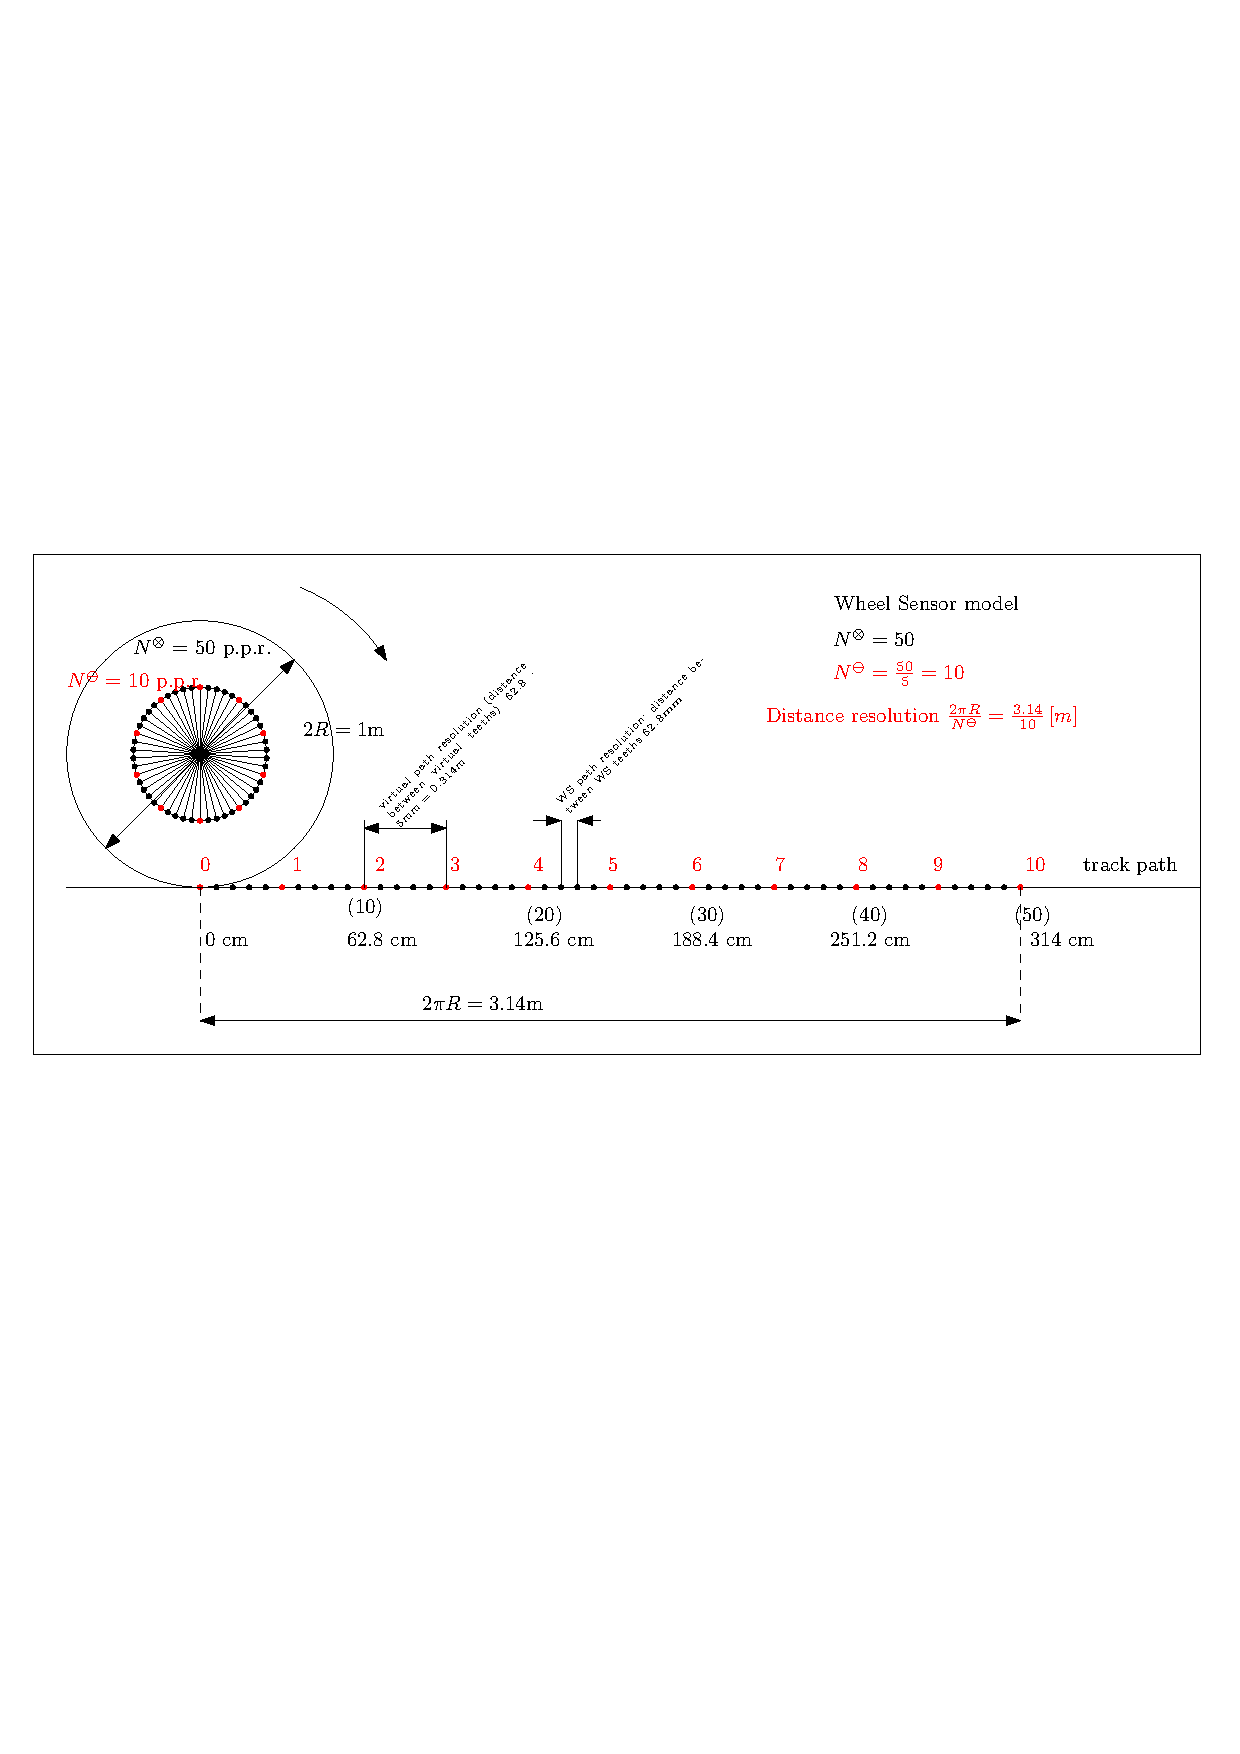
\includegraphics[angle=0,width=.9\textwidth]{virtual_teeths_v3.pdf}
}
\caption{\emph{virtual teeth and path resolution}}
\label {fig:virtualteeth}
\end{figure}
An alternative solution to improve the measurement performance at lower speed is to switch from frequency to period measurement e.g. below a certain level of (low) speed. The measurement is realized by counting the number of periods of a high frequency signal inside one (or more) encoder pulses, Fig. \ref{fig:periodenc}. The following formula is obtained under the hypothesis that motor speed is constant and only one period $\delta^\ominus_k N^\ominus = 1$ of the encoder signal is considered:
\begin{equation}
\omega=\frac{\mathrm{d}\theta}{\mathrm{d}t}\approx \frac{\delta^\ominus_k\theta}{\delta^\ominus_k\lambda^\star\cdot\tau^\star}= \left(\frac{2\pi}{N^\ominus}\right)\frac{1}{\lambda^\star_{,k^\ominus}\cdot\tau^\star}
\end{equation}

A speed sample $\lambda_k$ can be accumulated each period of the encoder signals. The speed sampling period is thus a function of wheel speed:
\begin{equation}
T^\ominus_k(\omega) =\delta^\ominus_k\lambda^\star\cdot\tau^\star = \left( \frac{2\pi}{N^\ominus}\right)  \frac{1}{\omega}=\frac{T_{\gls{WS}}(\omega)}{N^\ominus}
\end{equation}
where $\omega$ is the angular speed of the wheel and $T_{\gls{WS}}$ would be the period of a complete revolution of the wheel sensor at constant angular speed.
The accuracy of the measurement is related to the ratio between the period of the high frequency counter and that of the encoder signals, that is not an integer value as it depends on motor speed. A calculation of absolute and percentage errors is extremely difficult as it involves non-linear rounding functions.
A worst-case condition error could be calculated instead by considering the absolute error of one high frequency pulse, leading to a maximum percentage error limiting locus given by the following formula, i.e. roughly linear with speed:
\begin{equation}
e_k(\omega)=\frac{\tau^\star}{\frac{2\pi}{N^\otimes\cdot\omega}-\tau^\star} = \frac{\omega N^\ominus \tau^\star}{2\pi \left(1-N^\ominus\cdot\frac{\tau^\star}{T_{\gls{WS}}}\right)} \approx \frac{\omega\cdot N^\ominus\cdot \tau^\star}{2\pi}=\frac{N^\ominus\tau^\star}{T_{\gls{WS}}(\omega)} = \frac{\tau^\star}{T^\ominus_k(\omega)}
\end{equation}

(the factor $100$ is omitted)

At very low speed the number of high frequency pulses can be extremely high and %\colorbox{yellow}
{saturation} of the digital timer
employed for measurement can occur. Also a speed sample is not available each speed control period, needing an adaptation of the control parameters. In that situation, the quadrature decoding of the encoder pulses can be exploited in order to reduce the width of the measuring window by a factor of four or a reduction of the frequency of the timer can be considered.

The former solution allows to reduce the speed sampling period and improve the control performance of the drive, but makes the measuring system more sensitive to sensor
nonidealities, including variations in the transition locations
from their nominal values and phasing errors between encoder
channels. When low-cost and low-resolution sensors are
employed, nonidealities play the major role in the
determination of period measuring errors and has to be
carefully analyzed in drive design phase. The latter solution
needs to switch on-line the frequency of the timer and adapt the
coefficients of the equations above.
\begin{figure}[ht!]
\centerline{
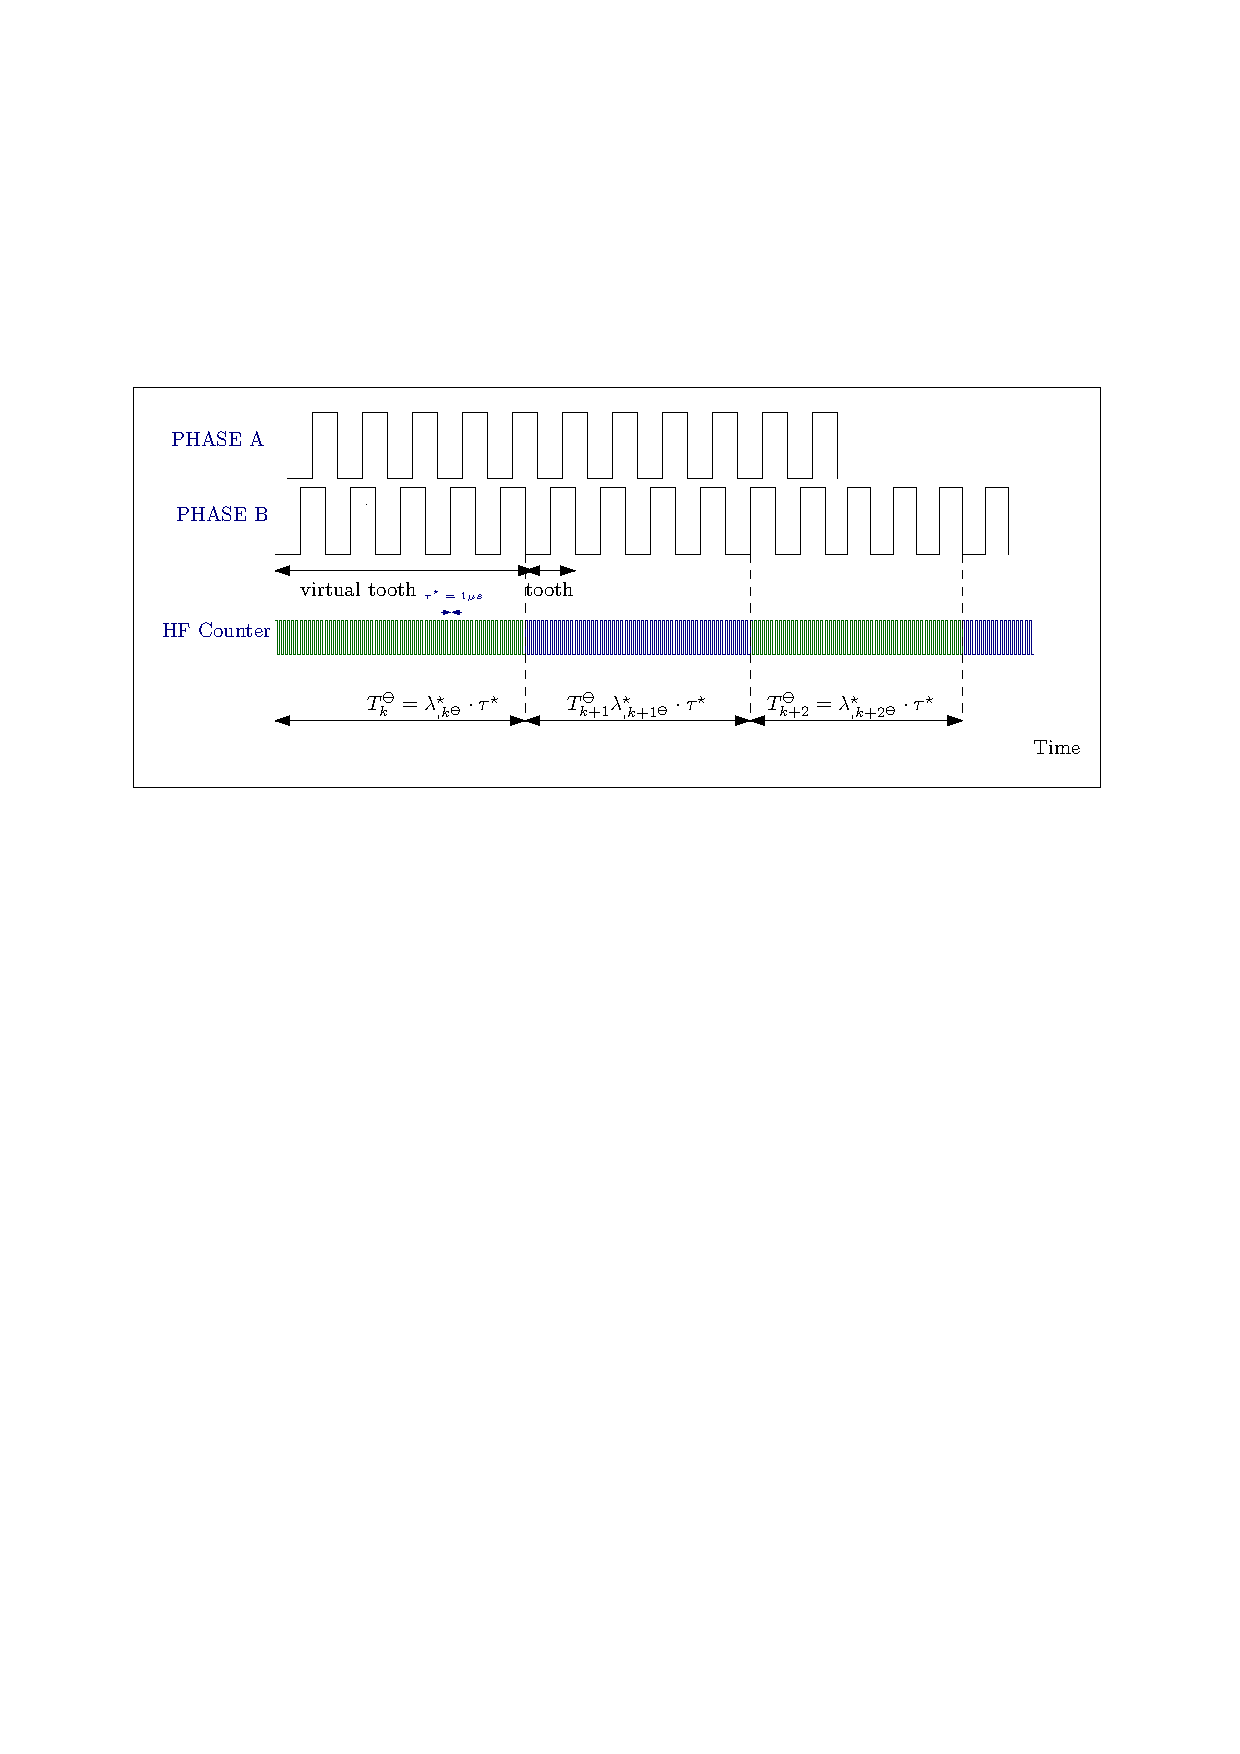
\includegraphics[angle=0,width=.7\textwidth]{period_m.pdf}
}
\caption{\emph{period measure}}
\label {fig:periodenc}
\end{figure}

The implementation of the period measuring method is also
straightforward as it requires a simple timer capture unit,
commonly found inside recent micro-controllers. Specific
hardware subsystems can be considered to overcome digital
timer saturation problems and proper
algorithms are needed to filter out the errors introduced by
sensor nonidealities. The problem of speed
calculation error generated at motor reversion can be easily
solved by the identification of motor direction during time
measurement and correction of the timer value, but best
performance are obtained by means of specific hardware
solutions.




\subsubsection{sensor data}
\paragraph{Delta path (\gls{MMU} cycle path increment)}\footnote {called also delta distance}
The \gls{MMU} processor executes a fetch cycle each $\tau^\circ=50\, \mathrm{m}s$. The samples which are available as raw data are used to calculate the path traveled on the last 50 ms. this is also called Delta-distance or path increment during cycle n.
\begin{equation}
\Delta^\circ_n s = R \Delta^\circ_n \theta = \left(\frac{2\pi R}{N^\ominus} \right) \Delta^\circ_n N^\ominus
\end{equation}
where $\Delta^\circ_n N $ \footnote{Later on where the context is clear we will drop the Delta symbol $\Delta$ and simply write $N^\ominus_{n^\circ}=N^\ominus_{n}$ to indicate the number os samples acquired in the \gls{MMU} cycle n.}  indicates the number of samples cumulated in the \gls{MMU} cycle n. 
\paragraph{current speed}
From the samples $\lambda_{n,k}$ where $n\in[0,\infty] $ is  the index of the \gls{MMU} cycle while $k\in[0,\Delta^\circ_n N^\ominus-1]$ is the index of the samples cumulated in the last cycle at virtual tooth border within the counter array,\footnote{The array has a size NB\_SAMPLES\_MAX, which limits the maximum number of samples, that can be stored in one cycle} the current speed on the cycle n can now be calculated:
\begin{equation}
\varv_{n^\circ} =\frac{\Delta^\circ _n s}{\sum\limits_{k=0}^{\Delta^\circ_n N^\ominus-1}\lambda^\star_{n,k}\tau^\star}  
\end{equation}
\paragraph{smoothed speed}
To avoid small oscillations of the speed due to the eccentricity of the fitted sensor relative to axle of rotation, the speed is smoothed over a full number of wheel revolutions while keeping a delay of 250 ms for the synchronization.
The raw samples of are transferred to a local buffer together with samples of previous cycles.
The sum of the last $N_{\tau^\bullet}$ raw samples (buffered locally) is chosen so that the sum of samples times $\tau^\star$ is immediately less than 500 ms (10 \gls{MMU} cycles) and $N_{\tau^\bullet}$ is a multiple of the number of virtual teeth $N^\ominus$ of the sensor.
\begin{equation}
\Delta^{\bullet}_n N^\ominus=N^\ominus \left\lfloor \frac {\sum\limits_{j=0}^{N^\bullet-1} \Delta^\circ_{n-j}{N^\ominus} }{N^\ominus}\right\rfloor 
\end{equation} 

Where the parenthesis $\left\lfloor \right\rfloor$ indicate integer part (floor). To obtain the raw speed, $\Delta^{\bullet}_n N$ is multiplied by the distance resolution and divided by this sum:
\begin{equation}
\widetilde{\varv}_{n^\bullet}=\frac{ \Delta^{\bullet}_n N^\ominus \left(\frac{2\pi R }{N^\ominus}\right)}{\sum\limits_{j=0}^{N^\bullet-1} \sum\limits_{k=0}^{\Delta^\circ_n N^\ominus-1}\lambda^\star_{n-j,k}\tau^\star}
\end{equation}
\begin{equation}
\widetilde{\varv}_{n^\bullet}=\frac{ \Delta^{\bullet}_n N^\ominus \left(\frac{2\pi R }{N^\ominus}\right)}{ \sum\limits_{\kappa=0}^{\Delta^\bullet_n N^\ominus-1}\lambda^\star_{,\kappa}\tau^\star}
\end{equation}


\begin{figure}[ht!]
\centerline{
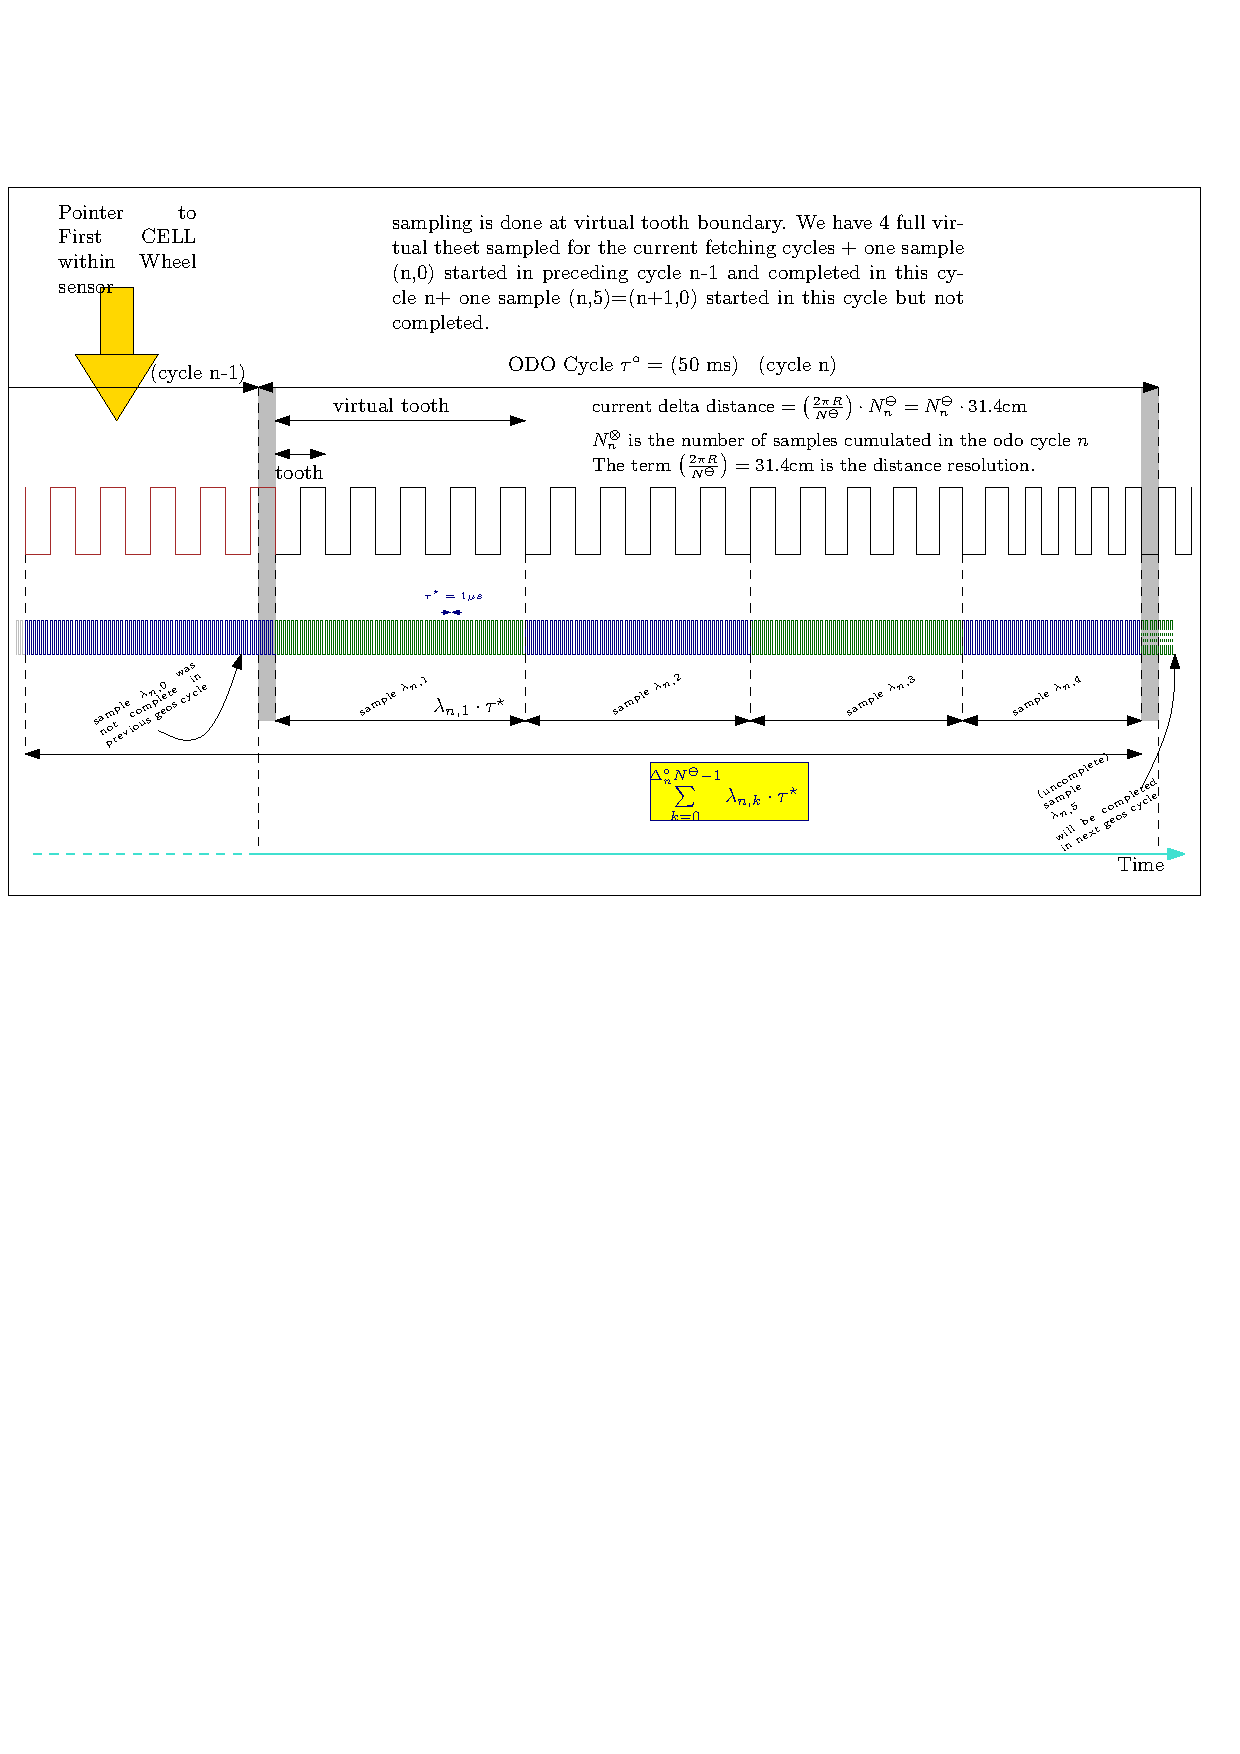
\includegraphics[angle=0,width=1.\textwidth]{teeth_v2.pdf}
}
\caption{\emph{sampling on a \gls{MMU} cycle}}
\label {fig:vteeth_samp}
\end{figure}
\paragraph{moving average over delta path}
The sensors output are to be synchronized every 250 ms. This is achieved by using a moving average on a period of time = (500ms – latency time). The latency time of the sensors has to be less than 250ms. Currently, the used sensors have a negligible latency time and so, the moving average is computed on 500 ms.
The speed estimation is computed using a smoothing mechanism over the speed measurements obtained during the last 500 ms leading to a delay of 250 ms on the speed estimation. The purpose of this mechanism is to smooth the speed measurement and to synchronize at 250 ms the speed estimations between the different
sensors.

The delta-path $(\Delta^\circ_n s )$ will now be averaged using a moving window over the last $N^\bullet$ sampled and stored $\Delta^\circ_{n-j} s$ values (impulses times wheel sensor resolution) acquired in the last 500 ms ($N^\bullet$ cycles = 10 data values).
The expression used for the moving average if we consider also the current value ($j=0$) is given by the formula:
\begin{equation}
\langle \Delta s\rangle^\bullet_n =\frac{1}{N^\bullet}\sum\limits_{j=0}^{N^\bullet-1} \Delta^\circ_{n-j} s 
\end{equation}
which can be updated recurrently at each cycle:
\begin{equation}
\langle \Delta s\rangle^\bullet_{n+1} =\langle \Delta s\rangle^\bullet_{n} +\frac{1}{N^\bullet}\left( \Delta^\circ_{n+1} s -  \Delta^\circ_{n-N+1} s \right)  
\end{equation}
where $N^\bullet=10$ is the size of the sampling buffer and the computation is extended over $N^\bullet$ values including the current data value ($j=0$). The index $n$ on the angular brackets indicates that the sample mean is done on the running buffer containing the data sample trailing the data value acquired at cycle $n$. The index $j$ gives the relative delay of the data point compared to the current data point $n$, while the index $i$ gives the number of the cycle where the data point was acquired, where the number of the fetching cycle has to be considered from the startup of the program, Usually such an index is not available and actual calculations should be made by using the relative index $j$ at each cycle $n$
The life span of a odometry increment is thus equal to 10 cycles. This allows to improve the resolution of the delta-path. The handling of vote mechanism for distance will be than performed voting over the values $\langle \Delta s\rangle^\bullet_{n} $ obtained using the formula above. The corresponding time value should be the one of the center of the averaging window, which is delayed by $j=N/2$ cycles relative to current fetch cycle.  The correct direction has to be associated to the distance increment.

\subsubsection{estimating acceleration from speed measures}

The acceleration can be estimated from the speed data sampled in the current buffer (sample n including current speed measure $\varv_n$) by implementing a linear regression on the sample.
Two possible linear estimators\footnote{\emph{regression} meaning the prevailing of the average over the fluctuations. The concept of \emph{regression to mediocrity}, introduced by Sir Galton reflects the behavior of data when numerous small effects influence and produce fluctuations superposed to systematic behavior. This behavior would certainly not be applicable to a random walk process.} are given by :
\begin{eqnarray}
\hat{\varv}(t_i) &=&\hat{\varv}_n+\hat{a}_n\left(t_i-t_n\right)\label{fig:lin_est1}\\
\hat{\varv}(t_i) &=&\hat{\varv}^{\spadesuit}_n+\hat{a}_n\left(t_i-\langle t \rangle_n\right) \label{fig:lin_est2}
\end{eqnarray}
where the index n indicates the value currently acquired and the associated trailing buffer storing another $N=2M$ sampled data. The total sample will have $N^\bullet$ data points $(\varv_i,t_i)$. The hat symbol will indicate estimated quantities e.g. $\hat{a}_n$ indicates the estimated acceleration over the sample n. There are two parameters to estimate $\hat{\varv}_n$ and $\hat{a}_n$.  The angular brackets indicate the mean value over the sample n obtained by averaging over the $N+1$ data points available at fetching cycle n. For the time value this is the arithmetic mean value (there is no statistical spread over the t variable and the fluctuation on the cycle time $\tau$ is considered negligible). Therefore this value is given only by the buffer size (time window) and can be calculated even without data.
\begin{eqnarray}
\langle t \rangle^\bullet_n &=& \frac{1}{N^\bullet}\sum\limits_{i=n}^{n-N^\bullet+1} t_i \nonumber \\ 
&=& \frac{1}{N^\bullet}\sum\limits_{j=0}^{N^\bullet-1} t_{n-j} \nonumber \\ 
&=& t_{n-N^\bullet/2} \nonumber\\
%&=&  t_{n-M} \nonumber\\
%&=&  t_n-M\tau \nonumber\\
&=&  t_n-\frac{N^\bullet}{2}\tau^\circ
\label{eq:mean_delay}
\end{eqnarray}
\begin{equation}
\boxed{
\langle t \rangle^\bullet_n = t_n-\frac{N^\bullet}{2}\tau
}
\end{equation}
and recurrently:
\begin{equation}
\langle t \rangle^\bullet_{n+1} = \langle t \rangle^\bullet_{n} +\tau^\bullet
\end{equation}

where $M\tau= N/2 \tau$ is the delay of the center of the buffering window (average delay) with respect to the current cycle.
in a similar way for the speed we have:
\begin{equation}
\langle \varv \rangle^\bullet_n=\frac{1}{N^\bullet}\sum\limits_{i=n}^{n-N^\bullet+1} \varv_i =\frac{1}{N^\bullet}\sum\limits_{j=0}^{N^\bullet-1} \varv_{n-j}
\end{equation}
which can be updated recurrently by:
\begin{equation}
\boxed{
\langle \varv \rangle^\bullet_{n+1}=\langle \varv \rangle^\bullet_n +\frac{1}{N^\bullet}\left( \varv_{n+1} - \varv_{n-N^\bullet+1}\right)
}
\end{equation}
\begin{figure}[h!]
\centerline{
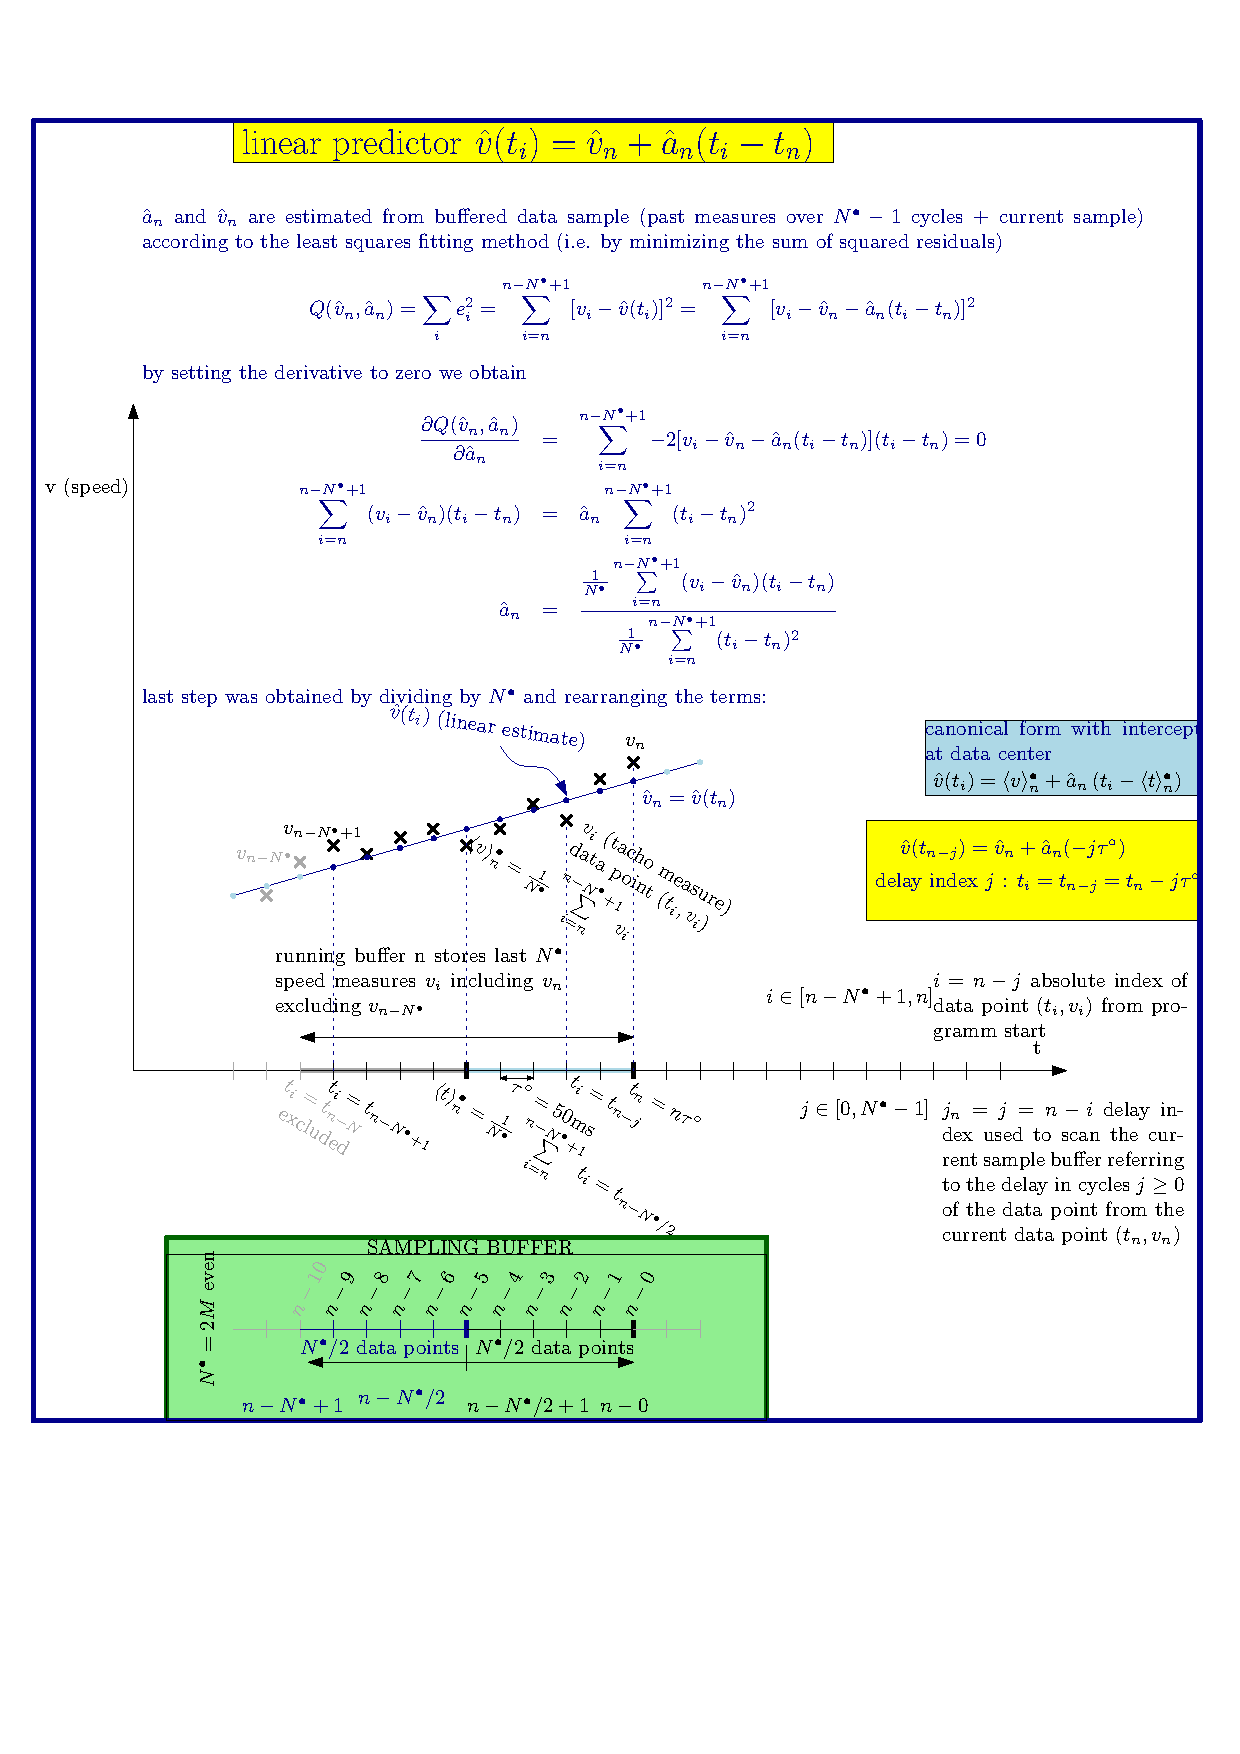
\includegraphics[angle=-0,width=1.\textwidth]{lin_regression_v7.pdf}
}
\caption{\emph{estimate acceleration applying linear regression}}
\label {fig:lregression}
\end{figure}


A way to estimate the parameters of the linear estimator consists in building an error function, aimed to produce a metric by summing up the distance or residual error between acquired data points and estimated data markers \cite{bevington}. This metric will allow to optimize the parameters for the smallest error. One of the most common error function is given by the sum of squared errors, the confidence interval of all data points being assumed identical. This is known as \emph{least square estimation}, and can be applied to a vast spectrum of (not only linear) functions containing parameters e.g. it si applicable for the coefficient estimation of any Fourier sum.

\begin{equation}
Q(\hat{\varv}_n, \hat{a}_n) =\sum\limits_{i=n}^{n-N^\bullet+1} e_i^2=\sum\limits_{i=n}^{n-N^\bullet+1}[ \varv_i-\hat{\varv}(t_i)]^2  =\sum\limits_{i=n}^{n-N^\bullet+1}[\varv_i-\hat{\varv}_n-\hat{a}_n(t_i-t_n)]^2
\end{equation}
We insert one of the selected estimators (\ref{fig:lin_est1}) in the $Q$ function, derive it and put the result to zero to locate the minimum.
\begin{equation}
\frac{\partial Q(\hat{\varv}_n, \hat{a}_n)}{\partial\hat{\varv}_n}=\sum\limits_{i=n}^{n-N^\bullet+1} 2\frac{\partial\hat{\varv}(t_i)}{\partial\hat{\varv}_n}[\varv_i-\hat{\varv}_n-\hat{a}_n(t_i-t_n)]=0
\end{equation}
dividing by $N^\bullet$ this gives:
\begin{eqnarray}
\hat{\varv}_n &=& \frac{1}{N^\bullet} \sum\limits_{i=n}^{n-N^\bullet+1} [\varv_i-\hat{a}_n(t_i-t_n)]\nonumber\\
&=& \langle \varv \rangle^\bullet_n-\hat{a}_n\left [\langle t\rangle^\bullet_n - t_n\right ]
\end{eqnarray}
In a similar way inserting the estimator (\ref{fig:lin_est2}) in the $Q$ function we obtain after derivation:
\begin{eqnarray}
\hat{\varv}^{\star}_n &=& \frac{1}{N^\bullet} \sum\limits_{i=n}^{n-N^\bullet+1} [\varv_i-\hat{a}_n(t_i-\langle t\rangle^\bullet _n)]\nonumber\\
&=& \langle \varv \rangle^\bullet_n
\end{eqnarray}
If we substitute the parameter $ \hat{\varv}_n $ in the original function we obtain in both cases:
\begin{equation}
\boxed{\color{blue}
\hat{\varv}(t_i) =\langle \varv \rangle^\bullet_n + \hat{a}_n\left(t_i-\langle t \rangle^\bullet_n\right)
}
\label{eq:lincan}
\end{equation}

centered on the center of data points sample $(\langle \varv \rangle^\bullet_n,\langle t \rangle^\bullet_n)$.\footnote{With increasing values of $n$ we get $N^\bullet$ different estimates $\hat{\varv}(t_i)$  for the same sample $\varv_i$, as the averaging window is moving forward in time.}
This is a 
%\colorbox{yellow}
{canonical form} for the linear predictor reflects the fact that the linear estimation function always includes
%\colorbox{yellow}
{the center} of the data sample. The second parameter $\hat{a}_n$ being the inclination of the line pivoting about the data sample center. 
The estimated value for the last sample is given by adding the estimated acceleration over the half window period to the window center velocity value $\varv(\langle t\rangle_n)=\langle \varv\rangle_n $
\begin{equation}
\hat{\varv}(t_n) =\langle \varv \rangle^\bullet_n + \hat{a}_n\frac{N^\bullet}{2} \tau^\circ
\end{equation}

The error function becomes:
\begin{equation}
\boxed{
Q(\hat{\varv}_n, \hat{a}_n) = \sum\limits_{i=n}^{n-N^\bullet+1}[ \varv_i-\langle \varv \rangle^\bullet_n - \hat{a}_n\left(t_i-\langle t \rangle^\bullet_n\right)]^2
}
\end{equation}
We use now this expression to get the estimation of the second parameter $\hat{a}_n$
\begin{equation}
\frac{\partial Q(\hat{\varv}_n, \hat{a}_n)}{\partial\hat{a}_n}=\sum\limits_{i=n}^{n-N^\bullet+1} 2\frac{\partial\hat{\varv}(t_i)}{\partial\hat{a}_n}[\varv_i-\langle \varv \rangle^\bullet_n -\hat{a}_n(t_i-\langle t\rangle^\bullet_n)]=0
\end{equation}
dividing by $N^\bullet$ and reordering we get
\begin{equation}
\frac{1}{N^\bullet}\sum\limits_{i=n}^{n-N^\bullet+1} [\varv_i-\langle \varv \rangle^\bullet_n -\hat{a}_n(t_i-\langle t\rangle^\bullet_n)](t_i-\langle t\rangle^\bullet_n)=0
\end{equation}

\begin{equation}
\boxed{
\hat{a}_n=\frac{\frac {1}{N^\bullet}\sum\limits_{i=n}^{n-N^\bullet+1}(\varv_i - \langle \varv \rangle^\bullet_n)(t_i-\langle t\rangle^\bullet_n)}{\frac {1}{N^\bullet} \sum\limits_{i=n}^{n-N^\bullet+1}(t_i- \langle t\rangle^\bullet_n)^2}=\frac{\langle \varv \cdot t\rangle^\bullet_n - \langle \varv \rangle^\bullet_n \langle t\rangle^\bullet_n}{\langle t^2\rangle^\bullet_n- \langle t \rangle^{\bullet 2}_n}
}
\label{eq:aest}
\end{equation}

the expression for $\langle t\rangle_n $ was already given in \ref{eq:mean_delay}. We still  need the expression for $\langle t^2\rangle_n$. Both $\langle t^2\rangle^\bullet_n$ and $\langle (t - \langle t^2\rangle^\bullet_n)^2\rangle^\bullet_n$ are characterized only by the buffer size and are data independent, while $\langle \varv \cdot t\rangle^\bullet_n$ and $\langle \varv \rangle^\bullet_n$ have to be evaluated from data.
\begin{eqnarray}
\frac {1}{N^\bullet}\sum\limits_{i=n}^{n-N^\bullet+1} (t_i - \langle t\rangle^\bullet_n)^2 &=&
\langle t^2\rangle^\bullet_n- \langle t\rangle^{\bullet 2}_n \nonumber\\
&=& \langle( t - \langle t\rangle^\bullet_n)^2\rangle^\bullet_n
\end{eqnarray}
Recalling that $ \langle t\rangle^\bullet_n = t_n-\frac{N^\bullet}{2}\tau^\circ$ we get:
\begin{eqnarray}
\frac {1}{N^\bullet}\sum\limits_{i=n}^{n-N^\bullet+1} \tau^{\circ 2} \left (i - n + \frac{N^\bullet}{2}\right )^2 &=&\nonumber\\
\frac { \tau^{\circ 2} }{N^\bullet}\sum\limits_{j=0}^{N^\bullet-1}(\frac{N^\bullet}{2}-j)^2 &=& \tau^{\circ 2} \frac{(N^\bullet-1)(N^\bullet+1)}{12}
\end{eqnarray}
where we have changed the index $i-n=-j$
\begin{equation}
\boxed{\color{blue}
\frac {1}{N^\bullet}\sum\limits_{i=n}^{n-N^\bullet+1} \left (t_i - \langle t\rangle^\bullet _n\right)^2=\tau^{\circ 2} \frac{(N^\bullet-1)(N^\bullet+1)}{12}
}
\end{equation}


In a similar fashion :
\begin{eqnarray}
\frac {1}{N^\bullet}\sum\limits_{i=n}^{n-N^\bullet+1} (t_i - \langle t\rangle^\bullet_n) &=&
\langle t - \langle t\rangle^\bullet_n\rangle^\bullet_n \nonumber\\
&=& \langle t \rangle^\bullet_n - \langle t\rangle^\bullet_n \nonumber\\ &=& 0
\end{eqnarray}

\clearpage
and so finally the equation \ref{eq:aest} becomes:  
\marginpar{\footnotesize $\Leftarrow $ by using: 
$$
\langle \varv \rangle_n\sum\limits_{i=n}^{n-N}(t_i-\langle t\rangle_n)=0
$$
}
\begin{eqnarray}
\hat{a}_n &=& \frac{\frac {1}{N^\bullet}\sum\limits_{i=n}^{n-N^\bullet+1}(\varv_i - \langle \varv \rangle^\bullet_n)(t_i-\langle t\rangle^\bullet_n)}{\frac {1}{N^\bullet} \sum\limits_{i=n}^{n-N^\bullet+1}(t_i- \langle t\rangle^\bullet_n)^2}\nonumber\\
&=& \frac{\frac {1}{N^\bullet}\sum\limits_{i=n}^{n-N^\bullet+1} \varv_i (t_i-\langle t\rangle^\bullet_n)}{\frac {\tau^{\circ 2} (N^\bullet-1)(N^\bullet+1)}{12} }\nonumber\\
&=& \frac{\frac {1}{N^\bullet}\sum\limits_{i=n}^{n-N^\bullet+1} \varv_i t_i -\frac {\langle t\rangle^\bullet_n }{N^\bullet}\sum\limits_{i=n}^{n-N^\bullet+1}\varv_i}{\frac {\tau^{\circ 2} (N^\bullet-1)(N^\bullet+1)}{12} }\nonumber\\
&=& \frac{\frac {1}{N^\bullet}\sum\limits_{j=0}^{N^\bullet-1} \varv_{n-j} t_{n-j} -\langle t\rangle^\bullet_n \langle \varv \rangle^\bullet_n}{\frac {\tau^{\circ 2} (N^\bullet-1)(N^\bullet+1)}{12} }\nonumber\\
&=& \frac{\frac {1}{N^\bullet}\sum\limits_{j=0}^{N^\bullet-1} \varv_{n-j} (t_n- j\tau^\circ) -\langle t\rangle^\bullet_n \langle \varv \rangle^\bullet_n}{\frac {\tau^{\circ 2} (N^\bullet-1)(N^\bullet+1)}{12} }\nonumber\\
&=& \frac{\frac {t_n}{N^\bullet}\sum\limits_{j=0}^{N^\bullet-1} \varv_{n-j} -\frac{\tau^\circ}{N^\bullet}\sum\limits_{j=0}^{N^\bullet-1} j\cdot \varv_{n-j} -\langle t\rangle^\bullet_n \langle \varv \rangle^\bullet_n}{\frac {\tau^{\circ 2} (N^\bullet-1)(N^\bullet+1)}{12} }\nonumber\\
&=& \frac{\langle \varv \rangle^\bullet_n (t_n-\langle t\rangle^\bullet_n ) -\frac{\tau^\circ }{N^\bullet}\sum\limits_{j=0}^{N^\bullet-1} j\cdot \varv_{n-j}}{\frac {\tau^{\circ 2} (N^\bullet-1)(N^\bullet+1)}{12} }\nonumber\\
&=& \frac{\langle \varv \rangle^\bullet_n \frac{\tau^\circ N^\bullet}{2} -\frac{\tau^\circ}{N^\bullet}\sum\limits_{j=0}^{N^\bullet-1} j\cdot \varv_{n-j}}{\frac {\tau^{\circ 2} (N^\bullet-1)(N^\bullet+1)}{12} }
\end{eqnarray}

\begin{equation}
\boxed{\color{blue}
\hat{a}_n= \left( \langle \varv \rangle^\bullet_n \frac{\tau^\circ N^\bullet}{2} -\frac{\tau^\circ}{N^\bullet}\sum\limits_{j=0}^{N^\bullet-1} j\cdot \varv_{n-j}\right) \frac {12}{\tau^{\circ 2} (N^\bullet-1)(N^\bullet+1)} 
}
\label{eq:aestls}
\end{equation}
which can be evaluated recurrently:
\begin{equation}
\boxed{\color{blue}
\hat{a}_{n+1}= \hat{a}_{n}+ \frac{6}{\tau^\circ }\frac{(N^\bullet-1)\varv_{n+1}-2N^\bullet\langle \varv\rangle^\bullet_n+(N^\bullet+1)\varv_{n-N^\bullet}}{ (N^\bullet-1)N^\bullet(N^\bullet+1)} 
}
\end{equation}

To obtain this relation simply substitute $n\rightarrow n+1$ in the definition \ref{eq:aestls}
\begin{equation}
\begin{array}{ll}
{\displaystyle \hat{a}_{n+1}} &{\displaystyle = \left( \langle \varv \rangle^\bullet_{n+1} \frac{N^\bullet}{2} -\frac{1}{N^\bullet}\sum\limits_{j=0}^{N^\bullet-1} j\cdot \varv_{n+1-j}\right) \frac {12}{\tau^\circ (N^\bullet-1)(N^\bullet+1)}} \\ 
&{\displaystyle = \left(\left( \langle \varv \rangle^\bullet_{n}+\frac{ \varv_{n+1}-\varv_{n-N^\bullet+1}}{N^\bullet} \right)\frac{N^\bullet}{2} -\frac{1}{N^\bullet}\sum\limits_{j=0}^{N^\bullet-1} j\cdot \varv_{n-(j-1)}\right) \frac {12}{\tau^\circ (N^\bullet-1)(N^\bullet+1)}} \\
&{\displaystyle = \left(\left( \langle \varv \rangle^\bullet_{n}+\frac{ \varv_{n+1}-\varv_{n-N^\bullet+1}}{N^\bullet} \right)\frac{N^\bullet}{2} -\frac{1}{N^\bullet}\sum\limits_{j=-1}^{N^\bullet-2} (j+1)\cdot \varv_{n-j}\right) \frac {12}{\tau^\circ (N^\bullet-1)(N^\bullet+1)}} \\
&{\displaystyle = \left(\left( \langle \varv \rangle^\bullet_{n}+\frac{ \varv_{n+1}-\varv_{n-N^\bullet+1}}{N^\bullet} \right)\frac{N^\bullet}{2} -\frac{\sum\limits_{j=0}^{N^\bullet-1} j\cdot \varv_{n-j}}{N^\bullet}+\varv_{n-N^\bullet+1}-\langle \varv\rangle^\bullet_n \right) \frac {12}{\tau^\circ (N^\bullet-1)(N^\bullet+1)}} \\
&{\displaystyle = \hat{a}_n+ \left( \frac{ \varv_{n+1}-\varv_{n-N^\bullet+1}}{N^\bullet} \frac{N^\bullet}{2} +\varv_{n-N^\bullet+1}-\langle \varv\rangle^\bullet_n \right) \frac {12}{\tau^\circ (N^\bullet-1)(N^\bullet+1)}} \\
&{\displaystyle = \hat{a}_n + \left( \frac{ \frac{N^\bullet}{2}\varv_{n+1}+\left(\frac{N^\bullet}{2}+1\right)\varv_{n-N^\bullet+1}-(N^\bullet)\langle \varv\rangle^\bullet_n}{N^\bullet} \right) \frac {12}{\tau^\circ (N^\bullet-1)(N^\bullet+1)}} \\
\end{array}
\end{equation}



\subsubsection{Goodness of fit}
If the deviations from the mean follow a Gaussian statistics, the probability of making any one observation $v_i$ at time $t_i$ is given by:
\begin{equation}
P(\varv_i)=\frac{1}{\sigma_i\sqrt{2\pi}}\exp\left (-\frac{\left [\varv_i-\mu(t_i)\right]^2}{2\sigma_i^2}\right)
\approx\frac{1}{\sigma_i\sqrt{2\pi}}\exp\left (-\frac{\left [\varv_i-\hat{\varv}(t_i)\right]^2}{2\sigma_i^2}\right)
\end{equation}
where we use the linear estimate $v(t_i)$ as estimate of the mean value $\mu(t_i)$ of the Gaussian being the value of velocity if measured at time $t_i$ with an hypothetical error-free device.
The total probability of obtaining a set of $N+1$ measurements,$ \{t_i ,\varv_i \}$, is
equal to the product of the probabilities for each data point:
\begin{equation}
\prod_{i=N-n}^nP(\varv_i)\approx\prod_{i=N-n}^n\left \{ \frac{1}{\sigma_i\sqrt{2\pi}}\exp\left (-\frac{\left [\varv_i-\hat{\varv}(t_i)\right]^2}{2\sigma_i^2}\right)\right\}
\end{equation}
\begin{figure}[h!]
\centerline{
%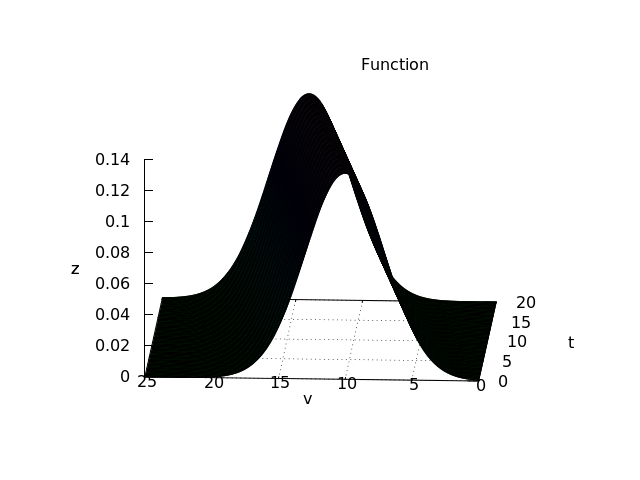
\includegraphics[angle=-0,width=.3\textwidth]{parent_pdf_d.png}
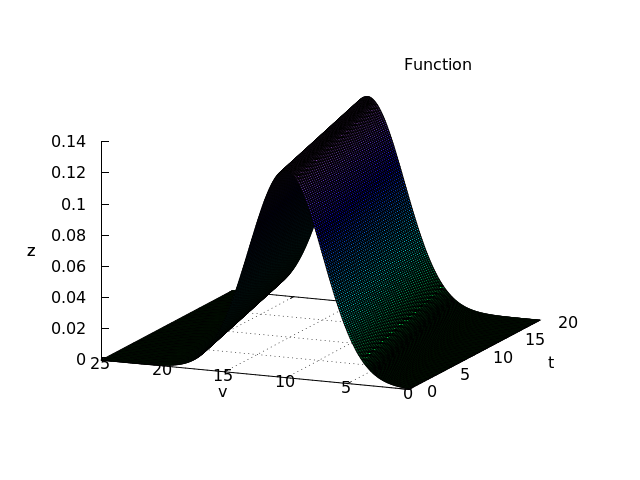
\includegraphics[angle=-0,width=.5\textwidth]{parent_pdf_a.png}
%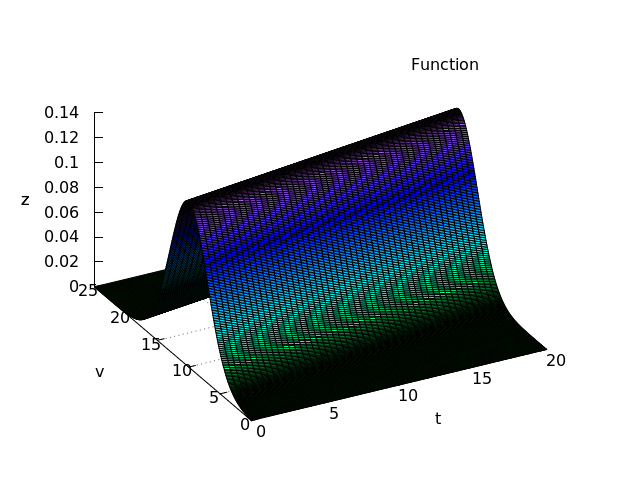
\includegraphics[angle=-0,width=.3\textwidth]{parent_pdf_b.png}
}
\caption{\emph{Gaussian family with "drifting" mean and constant variance}}
\label {fig:parent_pdf}
\end{figure}




\noindent
%%%%%%%%%%%%%%%
%%% INPUT:
%\begin{minipage}[t]{8ex}{\color{red}\bf
%\begin{verbatim}
%(%i36) 
%\end{verbatim}
%}
%\end{minipage}
%\begin{minipage}[t]{\textwidth}{\color{blue}
%\begin{verbatim}
%plot3d(1/(3*sqrt(2*%pi))*exp(-(v-10-0.2*t)^2/18), 
% [t,0,20], [v,0,25], [plot_format,gnuplot],
% [grid,50,350],
% [gnuplot_pm3d,true],
% [gnuplot_preamble, "set hidden3d"])$
%\end{verbatim}
%}
%\end{minipage}


Maximizing the probability is equivalent to minimize the sum in the exponential term of $ P (\{\varv,t\}) $ , specifically the sum of the deviations weighted by $\sigma^2_i$,
\begin{equation}
\sum\limits_{i=N-n}^n\frac{e_i^2}{2\sigma^2_i}=
\sum\limits_{i=N-n}^n\frac{\left [\varv_i-\hat{\varv}(t_i)\right]^2}{2\sigma^2_i}
\end{equation}
\footnote{ In case of variable variance $\sigma_i$ the expression to be maximized is
\begin{equation}
\prod\limits_{i=N-n}^n\frac{1}{\sqrt{2\pi}} exp\left( -\frac{\left [\varv_i-\hat{\varv}(t_i)\right]^2}{2\sigma^2_i}- \log\sigma_i\right)
\end{equation}
and therefore the exponent to be minimized is:
\begin{equation}
\sum\limits_{i=N-n}^n\left( \frac{\left [\varv_i-\hat{\varv}(t_i)\right]^2}{2\sigma^2_i}+ \log\sigma_i\right)
\end{equation}

But as we parametrize only the model estimating the mean value of $\hat{\varv(t_i)}$ the term $\log\sigma_i$ is a constant and can be ignored. The model predicts only the mean value and tries not to guess the variance interval.}
In the special case where all the $\sigma_i$ are identical we are we are led back to the least squares principle.
The chi-square statistic is defined by following sum where we replace the absolute index $i$ with the relative index $j$  $(i=n-j)$:
\begin{equation}
\boxed{
\chi^2=\sum\limits_{j=0}^{N}\frac{e_{n-j}^2}{\sigma^2_{n-j}}=
\sum\limits_{j=0}^{N}\frac{\left [\varv_{n-j}-\hat{\varv}(t_{n-j})\right]^2}{\sigma^2_{n-j}}
}
\end{equation}

If the terms of the sum are of the order of $\approx 1$ we get that $\chi$ increases with the number of observations $N+1$. The method of least squares is built on the hypothesis that the optimum
description of a set of data is one which minimizes the weighted sum of squares of deviations, $e_i$, between the data, $\varv_i$ , and the fitting function $\hat{\varv}(t_i)$.

The sum of squares of deviations is characterized by the “estimated variance of the fit”, $s^2$ , which is an estimate of the variance of the parent distribution, $\sigma^2$.
\begin{eqnarray}
s^2=\frac{1}{N+1}\sum\limits_{j=0}^{N} (\varv_{n-j}-\hat{\varv}(t_{n-j}))^2\nonumber\\
\sigma^2=\lim\limits_{N\to\infty}\frac{1}{N+1}\sum\limits_{j=0}^{N} (\varv_{n-j}-\mu(t_{n-j}))^2
\end{eqnarray}

The ratio of $s^2 /\sigma^2$ can be estimated by $\chi^2 / \nu$, where %\colorbox{yellow}
{ $ \nu  = N +1 - p $} is called degree of freedom, $N+1$ is the number of observations and $p$ is the number of fitting parameters. The expression $\chi^2 / \nu$ is called the 
%\colorbox{yellow}
{reduced chi-square} statistic.
For $p=2$ we get $\nu=N-1$ :
\begin{equation}
\boxed{
\frac{\chi^2}{\nu}=\frac{1}{N-1}\sum\limits_{j=0}^{N}\frac{\left [\varv_{n-j}-\hat{\varv}(t_{n-j})\right]^2}{\sigma^2_{n-j}}
}
\end{equation}

If the fitting function $\hat{\varv}(t_{n-j})$ accurately predicts the means $\mu(t_{n-j})$\footnote{the velocity at time $t_{n-j}$ measured with a much better device, having a much smaller error} of the parent distribution, then the estimated variance, $s^2$ , should agree well with the variance of the parent distribution, $\sigma^2$ , and their ratio should be close to one.
This explains the origin of the rule of thumb for chi-square fitting that states that a “good fit” is achieved when the reduced chi-square equals one.
The Chi-Square $(\chi^2 )$ distribution function gives the probability distribution for any quantity which is the sum of the squares of independent, normally-distributed variables with unit variance. In is used in the method of maximum likelihood for testing the functional relationship between measured quantities.
\begin{equation}
\boxed{
p(\chi^2,\nu)=\frac{1}{2^{\frac{\nu}{2}}\Gamma(\frac{\nu}{2})}\left(\chi^2\right)^{\frac{\nu-2}{2}}\exp\left[-\frac{\chi^2}{2}\right]
}
\end{equation}

Resuming the least squares method gives a general principle to obtain a fitting between a N-diemnsional vector $(v_i)$ of measured data with an N-dimensional vector produced by a model using 2 or more parameters. The parameters are used to assemble a linear combination of the base functions of the model space, they can be polynomial, periodic function or ...in the simplest case two parameters are used to produce a straight line. (linearity of the model space and linearity of function). There is no reference to any distribution or likelihood until here simply a minimum distance principle in the N-dimensional data space between observed vector $(\varv_0,\varv_1,\varv_2 \ldots \varv_N)$ and the synthetic vector $(\hat{\varv}(t_0),\hat{\varv}(t_1),\hat{\varv}(t_2),\ldots \hat{\varv}(t_N) )$
It emerges that if the data vector can be assumed to be subjected to an Gaussian error with constant variance, the least squares principle satisfies also a maximum likelihood principle. And the vector distance normalized by the factor $\sigma$ obeys a $\chi^2$ probability distribution function, which can be used to evaluate the  estimate the confidence interval. We define as above the error between the sampled speed and the speed value estimated with the linear regression:
\begin{equation}
e_i = \varv_i-\hat{\varv}(t_i) = \varv_i-\langle \varv \rangle_n + \hat{a}_n\left(t_i-\langle t \rangle_n\right)
\end{equation}
(see above \ref{eq:lincan}). and squaring:
\begin{equation}
e^2_i=(\varv_i-\langle \varv \rangle_n)^2+ 2(\varv_i-\langle \varv \rangle_n )(\hat{a}_n\left(t_i-\langle t \rangle_n\right)) + \hat{a}_n^2\left(t_i-\langle t \rangle_n\right)^2
\end{equation}

\begin{eqnarray}
\frac{1}{N+1}\sum\limits_{j=0}^{N}e^2_{n-j}&=&\frac{1}{N+1}\sum\limits_{j=0}^{N}(\varv_{n-j}-\langle \varv \rangle_n)^2\nonumber \\
&+& \frac{2}{N+1}\sum\limits_{j=0}^{N}(\varv_{n-j}-\langle \varv \rangle_n )(\hat{a}_n\left(t_{n-j}-\langle t \rangle_n\right))\nonumber \\ 
&+&\frac{1}{N+1}\sum\limits_{j=0}^{N}\hat{a}_n^2\left(t_{n-j}-\langle t \rangle_n\right)^2
\end{eqnarray}
\begin{eqnarray}
\frac{1}{N+1}\sum\limits_{j=0}^{N}e^2_{n-j}&=&\langle (v-\langle \varv \rangle_n)^2\rangle_n \nonumber \\
&+& 2\hat{a}_n\langle \left(v-\langle \varv \rangle_n \right)\cdot \left(t-\langle t \rangle_n\right)\rangle_n \nonumber \\ 
&+&\hat{a}_n^2\langle \left(t-\langle t \rangle_n\right)^2\rangle_n
\end{eqnarray}
  
the chi square indicates the variance of the error
\begin{equation}
\chi^2_{red}(e)=\frac{1}{N-1}\sum\limits_{j=0}^{N}e^2_{n-j}
\end{equation}

\subsection{measuring accelerations }
\begin{figure}[!ht]
%\boxed{
\centerline{
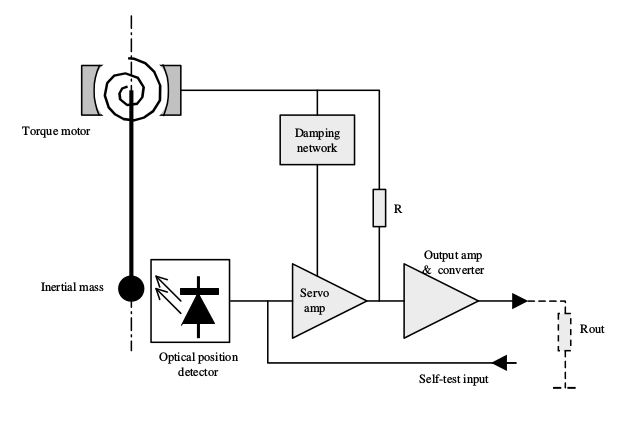
\includegraphics[angle=-0,width=.5\textwidth]{sensor.png}
}
%}
\caption{\emph{sketch of accelerometer}}
\label{fig:sensor}
\end{figure}
The accelerometer is intended to measure the acceleration along the train path (in tangent direction to the train path). The device  is calibrated in defined conditions when the train is in horizontal position and it is set up to have an equal elongation range for acceleration and for deceleration on a rectilinear route. 

It should be noticed, that if the train is moving freely downhill the acceleration measured by this device will be null, according to equivalence principle. On the other side if the train stands still with applied brake on a track with gradient the device will measure a deceleration given by $g\cdot\sin\iota\approx g\cdot\iota $, which will be of the order of $0.x \,\, m/s^2$ for typical gradient values. This effect corresponds to the braking force applied to the train to hold it still. 

This force is not producing work in the rest frame because there is no displacement and it is not producing work in any other reference because in the still stand the braking force compensates exactly the gradient force. 

If the train is accelerating by effect of traction force the measured value shall correspond to the (averaged) acceleration due to the traction. 
In other words the measured acceleration is only the contribution due to applied traction or brake but not the contribution from the gradient. In order to know the tangential acceleration component due to gradient we should (at least in theory) measure the acceleration component normal to the rail $g\cdot\cos\iota \approx g\cdot \left(1-\frac{1}{2}\iota^2 \right) $. 

The loss of weight would be only of the second order in the gradient and indicate a corresponding downhill acceleration or an uphill deceleration.


%\chapter{Bibliography}
\bibliographystyle{unsrt}
\bibliography{architecture}

\clearpage
%\chapter{Glossary}
%\addcontentsline{toc}{chapter}{Index}
%\printindex
% fill .glo file
%\glsaddall
% !!!! use tools glossary (F10)
\printglossary[type=\acronymtype, title=Acronyms, nonumberlist=true, style=altlong4colwithindent]
%\printglossary
%\printglossaries
%===================================================
%Do NOT change anything below this line

\end{document}
